\documentclass[12pt,a4paper]{report}
% ===== PRÉAMBULE =====
% ========================================
% PACKAGES DE BASE
% ========================================
\usepackage[utf8]{inputenc}                    % Encodage UTF-8 pour les caractères accentués
\usepackage[T1]{fontenc}                       % Encodage de sortie pour les polices européennes
\usepackage[french]{babel}                     % Support de la langue française

% ========================================
% PACKAGES MATHÉMATIQUES
% ========================================
\usepackage{mathtools}                         % Extension d'amsmath avec outils supplémentaires
\usepackage{amsfonts}                          % Polices mathématiques AMS
\usepackage{amssymb}                           % Symboles mathématiques AMS
\usepackage{amsthm}                            % Environnements de théorèmes
\usepackage{mathrsfs}                          % Lettres calligraphiques \mathscr{}
\usepackage{wasysym}
% ========================================
% PACKAGES GRAPHIQUES ET COULEURS
% ========================================
\usepackage{graphicx}                          % Inclusion et manipulation d'images
\usepackage[dvipsnames]{xcolor}                % Couleurs étendues (noms prédéfinis)
\usepackage{tikz}                              % Graphiques TikZ
\usepackage{tikz-cd}                           % Diagrammes commutatifs
\usetikzlibrary{calc}

% ========================================
% PACKAGES DE MISE EN PAGE
% ========================================
\usepackage[a4paper, margin=1in]{geometry}    % Configuration des marges
\usepackage{fancyhdr}                          % En-têtes et pieds de page personnalisés
\usepackage{titlesec}                          % Personnalisation des titres de sections
\usepackage{setspace}                          % Contrôle de l'interligne
\usepackage{titling} %Récupération du nom des auteurs                            
% Configuration détaillée des marges
\geometry{
    top=2.5cm,
    bottom=2.5cm,
    left=2.5cm,
    right=2.5cm,
    headheight=15.03pt,
    headsep=20pt,
    footskip=30pt
}

% ========================================
% PACKAGES DE MISE EN FORME
% ========================================
\usepackage{textcomp}                          % Symboles textuels supplémentaires
\usepackage{soul}                              % Soulignement et surlignage avancés
\usepackage{mdframed}                          % Boîtes encadrées personnalisables
\usepackage{tcolorbox}                         % Boîtes colorées avancées

% ========================================
% LISTES ET ÉNUMÉRATIONS
% ========================================
\usepackage[shortlabels]{enumitem}
\setlistdepth{9}
\renewlist{enumerate}{enumerate}{9}
\renewlist{itemize}{itemize}{9}

% Configuration des niveaux d'énumération
\setlist[enumerate,1]{label=(\roman*)}
\setlist[enumerate,2]{label=(\alph*)}
\setlist[enumerate,3]{label=\arabic*.}
\setlist[enumerate,4]{label=(\roman*)}
\setlist[enumerate,5]{label=(\alph*)}

% Configuration des niveaux d'itemize
\setlist[itemize,1]{label=$\bullet$}
\setlist[itemize,2]{label=$\circ$}
\setlist[itemize,3]{label=$-$}
\setlist[itemize,4]{label=$\ast$}

% ========================================
% HYPERLIENS
% ========================================
\definecolor{linkcolor}{RGB}{0,0,139}
\definecolor{citecolor}{RGB}{139,0,0}
\definecolor{urlcolor}{RGB}{0,100,0}

\usepackage[
    colorlinks=true,
    linkcolor=linkcolor,
    citecolor=citecolor,
    urlcolor=urlcolor,
    bookmarks=true,
    bookmarksnumbered=true,
    pdfstartview=FitH
]{hyperref}

% ========================================
% POLICES MATHÉMATIQUES
% ========================================
\usepackage{fouriernc}                         % Police Fourier
\DeclareMathAlphabet{\mathbb}{U}{msb}{m}{n}    % \mathbb standard (AMS)
\DeclareMathAlphabet{\mathcal}{OMS}{cmsy}{m}{n} % \mathcal standard

% ========================================
% STYLES POUR LES BOÎTES
% ========================================
\definecolor{lime}{RGB}{0,0,128}

% Macro pour définir des styles rapidement
\newcommand{\defstyle}[2]{\mdfdefinestyle{#1}{
    leftmargin=0pt,
    rightmargin=0pt,
    innerleftmargin=10pt,
    innerrightmargin=10pt,
    innertopmargin=0pt,
    innerbottommargin=2pt,
    leftline=true,
    rightline=false,
    topline=false,
    bottomline=false,
    linecolor=#2,
    linewidth=2pt,
    backgroundcolor=white
}}

% Styles spécifiques
\defstyle{definitionstyle}{RoyalBlue}
\defstyle{theoremstyle}{lime}
\defstyle{attentionstyle}{Red}

% Style classique (sans bordure colorée)
\mdfdefinestyle{classicstyle}{
    leftmargin=0pt,
    rightmargin=0pt,
    innerleftmargin=0pt,
    innerrightmargin=0pt,
    innertopmargin=0pt,
    innerbottommargin=2pt,
    leftline=true,
    rightline=false,
    topline=false,
    bottomline=false,
    linecolor=white,
    linewidth=2pt,
    backgroundcolor=white
}

% ========================================
% ENVIRONNEMENTS DE THÉORÈMES
% ========================================

% Définitions et axiomes
\newmdtheoremenv[style=definitionstyle,nobreak=true]{definition}{Définition}[section]
\newmdtheoremenv[style=definitionstyle,nobreak=true]{axiome}[definition]{Axiome}
\newmdtheoremenv[style=definitionstyle,nobreak=true]{conjecture}[definition]{Conjecture}
\newmdtheoremenv[style=definitionstyle,nobreak=true]{convention}[definition]{Convention}

% Théorèmes et résultats
\newmdtheoremenv[style=theoremstyle,nobreak=true]{theoreme}[definition]{Théorème}
\newmdtheoremenv[style=theoremstyle,nobreak=true]{lemme}[definition]{Lemme}
\newmdtheoremenv[style=theoremstyle,nobreak=true]{proposition}[definition]{Proposition}
\newmdtheoremenv[style=theoremstyle,nobreak=true]{corollaire}[definition]{Corollaire}
% Style amsthm
\newtheoremstyle{remarkstyle}
  {}{}
  {\normalfont}  % corps en droit
  {}
  {\itshape\bfseries}     % titre en italique
  {.}{ }{}

% Environnements auxiliaires
\theoremstyle{remarkstyle}
\newtheorem{remarque}[definition]{Remarque}
\surroundwithmdframed[style=classicstyle]{remarque}
% Style amsthm
\newtheoremstyle{normalstyle}
  {}{}
  {\normalfont}  % corps en droit
  {}
  {\normalfont\bfseries}     % titre en italique
  {.}{ }{}

% Environnements auxiliaires
\theoremstyle{normalstyle}
\newtheorem{exercice}[definition]{Exercice}
\surroundwithmdframed[style=classicstyle]{exercice}
\newtheorem{exemple}[definition]{Exemple}
\surroundwithmdframed[style=classicstyle]{exemple}
\newtheorem*{resolution}{Résolution}
\surroundwithmdframed[style=classicstyle]{resolution}
\newtheorem*{notation}{Notation}
\surroundwithmdframed[style=classicstyle]{notation}

% ========================================
% EN-TÊTES ET PIEDS DE PAGE
% ========================================
\pagestyle{fancy}
\fancyhf{}
\fancyhead[L]{\textit{\leftmark}}              % Chapitre à gauche
\fancyfoot[L]{\thepage}                        % Numéro de page à gauche
\fancyfoot[R]{\textit{\rightmark}}             % Section à droite

\renewcommand{\headrulewidth}{0pt}
\renewcommand{\footrulewidth}{0pt}

% Marques de chapitres et sections
\renewcommand{\chaptermark}[1]{%
    \markboth{\MakeUppercase{\chaptername\ \thechapter.\ #1}}{}}
\renewcommand{\sectionmark}[1]{%
    \markright{\MakeUppercase{\thesection.\ #1}}}

% Style pour les premières pages de chapitre
\fancypagestyle{plain}{%
    \fancyhf{}
    \fancyfoot[L]{\thepage}
    \fancyfoot[R]{\textit{\rightmark}}
}

% ========================================
% FORMAT DES TITRES DE SECTIONS
% ========================================
\titleformat{\chapter}[block]
    {\normalfont\LARGE\bfseries\scshape\color{RoyalBlue}\flushleft}
    {\thechapter.}
    {1em}
    {\scshape\color{RoyalBlue}}

\titleformat{\section}[block]
    {\normalfont\large\scshape\color{RoyalBlue}\flushleft}
    {\thesection}
    {1em}
    {}

\titleformat{\subsection}[block]
    {\normalfont\large\scshape\color{RoyalBlue}\flushleft}
    {\thesubsection}
    {1em}
    {}

\titleformat{\subsubsection}[block]
    {\normalfont\large\scshape\color{RoyalBlue}\flushleft}
    {\thesubsubsection}
    {1em}
    {}

% ========================================
% ENSEMBLES USUELS
% ========================================
\newcommand{\N}{\mathbb{N}}                    % Entiers naturels
\newcommand{\Z}{\mathbb{Z}}                    % Entiers relatifs
\newcommand{\Q}{\mathbb{Q}}                    % Rationnels
\newcommand{\R}{\mathbb{R}}                    % Réels
\newcommand{\C}{\mathbb{C}}                    % Complexes
\newcommand{\K}{\mathbb{K}}                    % Corps quelconque
\newcommand{\Sg}{\mathfrak{S}}                 % Groupe symétrique
\newcommand{\sn}{\mathbb{S}_n}                 % Sphère de dimension n

% ========================================
% LOGIQUE
% ========================================
\newcommand{\ssi}{\Leftrightarrow}             % Si et seulement si
\newcommand{\alors}{\Rightarrow}               % Implique
\newcommand{\si}{\Leftarrow}                   % Est impliqué par

% ========================================
% NORMES ET DISTANCES
% ========================================
\newcommand{\norm}[1]{\left\| #1 \right\|}     % Norme
\newcommand{\norme}[1]{\lVert #1 \rVert}       % Norme (variante)
\newcommand{\abs}[1]{\left| #1 \right|}        % Valeur absolue

% ========================================
% INTERVALLES
% ========================================
\newcommand{\interoo}[1]{\left] #1\right[}  % ]a,b[
\newcommand{\interof}[1]{\left] #1\right]}   % ]a,b]
\newcommand{\interfo}[1]{\left[ #1\right[}   % [a,b[
\newcommand{\interff}[1]{\left[ #1\right]}   % [a,b]

% ========================================
% TOPOLOGIE
% ========================================
\newcommand{\topologie}{\mathcal{T}}           % Topologie
\newcommand{\voisinage}{\mathcal{V}}           % Voisinages
\newcommand{\partie}{\mathscr{P}}              % Parties
\newcommand{\filtre}{\mathscr{F}}              % Filtre
\newcommand{\ouvert}{\mathcal{O}}              % Ouverts
\newcommand{\ferme}{\mathcal{F}}               % Fermés
\newcommand{\adh}{\operatorname{adh}}                % Adhérence
\DeclareMathOperator{\Cond}{Cond}               %Points de condensation
% ========================================
% FONCTIONS
% ========================================
\newcommand{\fonction}[3]{#1\colon \left\{\begin{array}{l}#2 \\#3\end{array}\right.}

% ========================================
% OPÉRATEURS MATHÉMATIQUES
% ========================================
\DeclareMathOperator{\dom}{dom}               % Domaine
\DeclareMathOperator{\im}{Im}                 % Image
\DeclareMathOperator{\e}{e}                   % Exponentielle
\DeclareMathOperator{\stab}{St}               % Stabilisateur
\DeclareMathOperator{\orb}{Orb}               % Orbite
\DeclareMathOperator{\coker}{coker}           % Conoyau
\DeclareMathOperator{\sgn}{sgn}               % Signature
\DeclareMathOperator{\Frac}{Frac}             % Corps des fractions
\DeclareMathOperator{\Eq}{Eq}                 % Égaliseur
\DeclareMathOperator{\Coeq}{Coeq}             % Coégaliseur
\DeclareMathOperator{\Cone}{Cone}             % Catégorie des cônes
\DeclareMathOperator{\colim}{colim}           % Colimite

% Limites avec indices
\newcommand{\limi}{\lim\limits}

% Intégrale différentielle
\newcommand{\intd}{\,\operatorname{d}}
\newcommand{\dpart}[2]{\frac{\partial #1}{\partial #2}}

% ========================================
% THÉORIE DES CATÉGORIES
% ========================================

% --- Catégories standards ---
\newcommand{\Set}{\mathbf{Set}}               % Ensembles
\newcommand{\Grp}{\mathbf{Grp}}               % Groupes
\newcommand{\Ab}{\mathbf{Ab}}                 % Groupes abéliens
\newcommand{\Ring}{\mathbf{Ring}}             % Anneaux
\newcommand{\CRing}{\mathbf{CRing}}           % Anneaux commutatifs
\newcommand{\Mod}{\mathbf{Mod}}               % Modules
\newcommand{\Vect}{\mathbf{Vect}}             % Espaces vectoriels
\newcommand{\Top}{\mathbf{Top}}               % Espaces topologiques
\newcommand{\Pos}{\mathbf{Pos}}               % Ensembles ordonnés
\newcommand{\Cat}{\mathbf{Cat}}               % Catégories
\newcommand{\Mon}{\mathbf{Mon}}               % Monoïdes

% --- Constructions ---
\newcommand{\Disc}{\mathbf{Disc}}             % Catégorie discrète
\newcommand{\op}{^{\mathrm{op}}}              % Catégorie opposée

% --- Objets et morphismes ---
\newcommand{\Ob}{\mathrm{Ob}}                 % Objets
\newcommand{\Hom}{\mathrm{Hom}}               % Morphismes
\newcommand{\End}{\mathrm{End}}               % Endomorphismes
\newcommand{\Aut}{\mathrm{Aut}}               % Automorphismes
\newcommand{\id}{\mathrm{id}}                 % Identité
\newcommand{\Id}{\mathrm{Id}}                 % Foncteur identité

% --- Groupes linéaires ---
\newcommand{\GL}{\mathrm{GL}}                 % Groupe linéaire général
\newcommand{\SL}{\mathrm{SL}}                 % Groupe spécial linéaire

% ========================================
% TOPOLOGIE ALGÉBRIQUE
% ========================================

% --- Espaces classiques ---
\newcommand{\Sph}[1]{S^{#1}}                  % Sphère S^n
\newcommand{\Boule}[1]{D^{#1}}                % Boule D^n
\newcommand{\Tore}{T^2}                        % Tore
\newcommand{\RP}[1]{\mathbb{RP}^{#1}}         % Espace projectif réel
\newcommand{\CP}[1]{\mathbb{CP}^{#1}}         % Espace projectif complexe
\newcommand{\simplex}{\Delta}                  % Simplexe standard

% --- Groupes d'homotopie ---
\newcommand{\pifond}[2]{\pi_1(#1,#2)}         % π₁(X,x₀)
\newcommand{\pihomo}[2]{\pi_{#1}(#2)}         % πₙ(X)

% --- Homologie et cohomologie ---
\newcommand{\Hsing}[1]{H_{#1}}                % Homologie H_n
\newcommand{\Cohsing}[1]{H^{#1}}              % Cohomologie H^n
\newcommand{\Htilde}[1]{\widetilde{H}_{#1}}   % Homologie réduite

% --- Complexes de chaînes ---
\newcommand{\Csing}[1]{C_{#1}}                % Chaînes singulières C_n
\newcommand{\Zsing}[1]{Z_{#1}}                % Cycles Z_n
\newcommand{\Bsing}[1]{B_{#1}}                % Bords B_n

% --- Relations ---
\newcommand{\iso}{\cong}                       % Isomorphisme
\newcommand{\rel}{\,\text{rel}\,}             % Relatif à

% ========================================
% NOTATIONS DIVERSES
% ========================================
\newcommand{\xn}{(x_n)_{n\in I}}              % Suite indexée par I
\newcommand{\yn}{(y_n)_{n\in J}}              % Suite indexée par J
\newcommand{\ie}{\textit{i.e.}}
%Pour la page de garde
\newcommand{\teacher}{C.Michaux}
\title{Topologie et    \: logique}
\author{T. Piette \and M.Hamiot}
\newcommand{\grade}{BaB2}

\begin{document}

% =====PAGE DE GARDE=====
\definecolor{encre}{RGB}{28,28,30}
\definecolor{accent}{RGB}{90,110,140}
\begin{titlepage}
\thispagestyle{empty}

% ---------- Filigrane : le cercle d'Apollonius ----------
\begin{tikzpicture}[remember picture, overlay]
  \node[opacity=0.16] at ($(current page.center)+(0,-0.6cm)$)
    {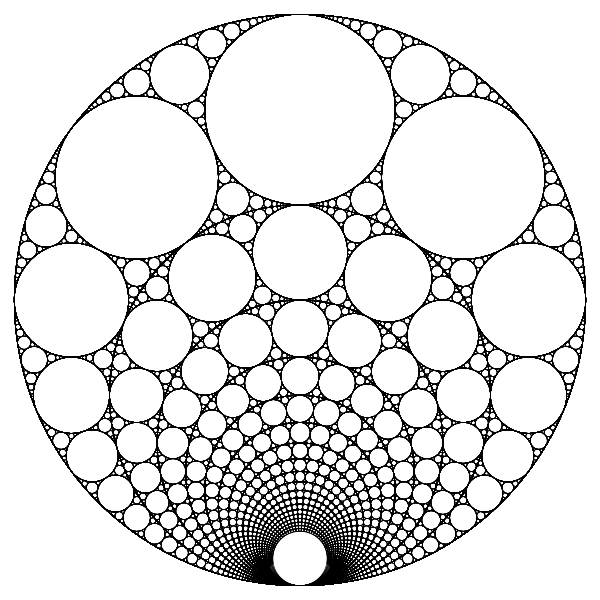
\includegraphics[width=17cm]{apollonius.png}};
\end{tikzpicture}

% ---------- Contenu ----------
\begin{center}
\vspace*{2.2cm}

{\footnotesize\color{accent}\scshape\selectfont
 \setlength{\baselineskip}{1.6em}
 Université de Mons \quad$\cdot$\quad Faculté des Sciences\par}

\vspace{3.4cm}

{\color{accent}\rule{2.2cm}{0.8pt}}

\vspace{1.1cm}

{\fontsize{43}{50}\selectfont\color{encre}
 Topologie et logique\par}

\vspace{1.0cm}

{\large\color{encre} Notes de cours\par}

\vspace{0.9cm}

{\color{accent}\rule{2.2cm}{0.8pt}}

\vfill

{\normalsize\color{encre}\scshape Tiago Piette \& Manoa Hamio\par}
\vspace{0.35cm}
{\footnotesize\color{accent}BaB2 --- Sciences mathématiques\par}
\vspace{0.15cm}
{\footnotesize\color{accent}2025\,--\,2026\par}

\vspace{1.4cm}
\end{center}

\end{titlepage}



%% PREFACE

\chapter*{Préface}
\addcontentsline{toc}{chapter}{Préface}

Le présent document constitue le syllabus du cours \textit{Topologie et Logique C.~Michaux}, dispensé au premier quadrimestre (Q1) de l’année académique 2025-2026 aux étudiants de deuxième année de bachelier (BAC2).

\vspace{0.5em}

Nous avons entrepris cette retranscription à partir des notes et exposés du cours donné par C.~Michaux, avec la volonté de proposer un support à la fois fidèle à l’esprit des séances et structuré de manière à en faciliter l’étude. Notre travail n’a pas pour ambition de remplacer le cours, mais d’en offrir une trace écrite claire et organisée, permettant de retrouver les définitions, résultats et idées essentielles développés tout au long du quadrimestre.

\vspace{0.5em}

Le contenu s’articule autour de deux axes fondamentaux. La première partie est consacrée à la logique et à la théorie des ensembles, qui constituent le socle formel des mathématiques modernes. La seconde partie est dédiée à la topologie.

\vspace{0.5em}

Les annexes rassemblent le contenu des présentations réalisées par les étudiants au second quadrimestre (Q2). Elles prolongent et enrichissent le cours en approfondissant certains thèmes, tant du côté de la logique et de la théorie des ensembles que de celui de la topologie.

\vfill

\vspace{1.5cm}

\begin{flushright}
    \textit{Mons, le \today} \\
    \textbf{M.Hamiot \& T.Piette}
\end{flushright}

\newpage

% ===== TABLE DES MATIÈRES =====
\tableofcontents
\newpage

% ===== CHAPITRES =====
\chapter{Éléments de théorie des ensembles}

\section{Théorie des ensembles Zermolo Fraenkel (ZF)}

\subsection{Paradoxe de Russel}
Jusqu'au début du XX\,\textsuperscript{e}~siècle, les mathématiciens manipulaient les ensembles de manière dite \emph{naïve}.
On les concevait d’abord comme des objets géométriques (points, droites, cercles, etc.), puis comme de simples collections d’objets partageant une propriété commune.

C’est le mathématicien allemand \textsc{Georg Cantor} (1845–1918) qui, à partir de 1874, posa les bases de la \emph{théorie naïve des ensembles}.
Cette approche intuitive permit à Cantor de développer la notion de \emph{cardinalité} et d’étudier différents « types d’infini » par des travaux qui révolutionnèrent les fondements des mathématiques modernes.
Cependant, cette théorie, bien que féconde, se révéla insuffisamment rigoureuse.

\medskip

En 1901, le philosophe et logicien britannique \textsc{Bertrand Russell} (1872–1970) mit en évidence une contradiction au cœur même de la théorie naïve : le \emph{paradoxe de Russell}.
Considérons l’ensemble suivant :
\[
	R := \{\,x \text{ ensemble} \mid x \notin x\,\}.
\]
Autrement dit, $R$ désigne l’ensemble de tous les ensembles qui ne se contiennent pas eux-mêmes.
La question est alors : $R$ appartient-il à lui-même~?

\medskip

\noindent
Deux cas se présentent :
\begin{itemize}
	\item Si $R \in R$, alors par définition de $R$, on doit avoir $R \notin R$.
	\item Si $R \notin R$, alors, toujours par définition, $R$ satisfait la condition pour appartenir à $R$ ; donc $R \in R$.
\end{itemize}
 On aboutit à la contradiction suivante :
\begin{equation*}
	R \in R \;\Longleftrightarrow\; R \notin R.
\end{equation*}

Cette impossibilité logique révèle une faille fondamentale de la théorie naïve : certaines définitions « trop générales » engendrent des paradoxes.

\medskip

Pour surmonter cette difficulté, les mathématiciens entreprirent de fonder la théorie des ensembles sur une base axiomatique rigoureuse.
En 1908, \textsc{Ernst Zermelo} (1871–1953) proposa une première axiomatisation visant à éviter les paradoxes.
Cette théorie fut ensuite enrichie en 1922 par \textsc{Abraham Fraenkel} (1891–1965) et, indépendamment, par \textsc{Thoralf Skolem} (1887–1963).
L’ensemble de ces axiomes constitue la théorie des ensembles \textbf{ZF} (\emph{Zermelo–Fraenkel}).
Lorsqu’on y ajoute l’axiome du choix (dont nous parlerons plus tard), on obtient la théorie \textbf{ZFC}, aujourd’hui la base de la plupart des mathématiques formelles.

\medskip

Cependant, même la théorie ZF ne permet pas de manipuler des « collections trop grandes » comme la collection de tous les ensembles, car celle-ci n'est pas un ensemble.
Pour traiter de telles collections, d’autres systèmes ont été développés, notamment la théorie \textbf{NBG} (\emph{von Neumann–Bernays–Gödel}), qui étend ZF en introduisant une distinction explicite entre ensembles et classes.
Dans ce chapitre, nous allons réaliser une brève introduction à la théorie ZF, théorie qui sera, sans doute, approfondie lors d'une présentation au Q2. Le but de ce document est simplement d'établir des propriétés ensemblistes nécéssaires pour les chapitres suivants, ainsi que d'introduire la notion de cardinalité qui sera également détaillée lors d'une présentation.

\subsection{Axiomatique et conséquences}

Dans la section suivante, nous énoncerons les axiomes qui constituent la théorie ZF et nous allons brièvement constater leurs conséquences directes. Il faut noter que cette section a été légèrement plus détaillée que ce que nous avons pu étudier pendant le cours.
Commençons par donner cinq axiomes dont les énoncés sont relativement aisés à comprendre et qui sont en accord avec l'intuition commune.

\section*{Axiomes élémentaires}

\begin{axiome}[d'extensionnalité]\label{ens : axiome : ext}
	Deux ensembles possédant les mêmes éléments sont égaux :
	\begin{equation*}
		\forall A,\forall B, \quad [\forall x, \: (x\in A \Leftrightarrow x\in B)] \: \Leftrightarrow \:A=B
	\end{equation*}
\end{axiome}
\begin{proposition}\label{ens : axiome : transi_égalité}
    Soient $A,B,C$ des ensembles. Si $A = B$ et $B=C$, alors $A=C$.
\end{proposition}
\begin{proof}
Soit $x$.
Considérons les expressions logiques $P\equiv x\in A, Q\equiv x\in B$ et $R\equiv x\in C$.
 Par table de vérité, on a $(P\ssi Q)\land(Q\ssi R)\alors P\ssi R$.
\end{proof}
\begin{axiome}[de l'ensemble vide]\label{ens : axiome ; vide}
	Il existe un ensemble qui ne contient aucun éléments :
	\begin{equation*}
		\exists E,\: \forall x,\: x\notin E
	\end{equation*}
\end{axiome}

\begin{proposition}
	Il n'y a qu'un seul ensemble qui ne possède aucun élément.
	On l'appelle ensemble vide et on le note $\varnothing$.
\end{proposition}

\begin{proof}
	Cela résulte des deux axiomes précédents.
\end{proof}
\begin{proposition}[Axiome de la paire]\label{ens : axiome : paire}
	Pour tous ensembles $a$ et $b$, il existe un ensemble, noté $\{a,b\}$
	, admettant comme éléments $a$ et $b$ et rien d'autre.
	\begin{equation*}
		\forall a,\forall b,\quad \exists E,\forall x, [x\in E \Leftrightarrow (x=a \lor x=b)]
	\end{equation*}
\end{proposition}
\begin{remarque}
Lorsque la théorie des ensembles était à ses débuts, cette proposition constituait un axiome. Puis, lorsque l'axiome de remplacement \ref{ens : axiome : remplacement} a été adopté, il n'était plus nécessaire. La preuve de cette proposition se trouve au point \ref{ens : axiome : preuve_paire}.
\end{remarque}

\begin{proposition}\label{ens: singleton}
	Pour tout ensemble $a$, il existe un ensemble et un seul dont $a$ est le seul élément. Cet ensemble est noté $\{a\}$
\end{proposition}

\begin{proof}
	Il s'agit d'un cas particulier de l'axiome de la paire avec $a=b$.
\end{proof}


\begin{axiome}[de la réunion]\label{ens : axiome : réunion}
	Pour tout ensemble $I$, il existe un ensemble $U$ dont les éléments sont les éléments des éléments $I$.
	\begin{equation*}
		\forall I,\exists U,\forall x, [x\in U \Leftrightarrow \exists i,(i\in I\land x\in i)]
	\end{equation*}
	L'ensemble $U$ est appelé la réunion des éléments de $I$, et on le note $\bigcup I$
\end{axiome}
Par exemple, si $I=\{\{a,b\}, \{c,d\},\{d\}\}$ alors $U= \{a,b,c,d\}$. 
\begin{definition}
	Soient $A$ et $B$ deux ensembles, on définit l'union de $A$ et $B$, que l'on note $A\cup B$, par l'ensemble $\bigcup I$ où $I=\{A,B\}$.
\end{definition}
\begin{definition}
	On dit qu'un ensemble $A$ est contenu dans un ensemble $B$, ou que $A$ est une partie de $B$ si tout élément de $A$ est élément de $B$.
	\begin{equation*}
		\forall x,[x\in A \Rightarrow x\in B]
	\end{equation*}
	On écrit alors $A\subseteq B$
\end{definition}

\begin{remarque}
	Il vient naturellement de cette définition que deux ensembles $A$ et $B$ sont égaux si et seulement si il sont inclus l'un a l'autre, c'est à dire
	$A=B \Leftrightarrow (A\subseteq B) \land ( B\subseteq A)$
\end{remarque}

\begin{axiome}[de l'ensemble des parties]\label{ens : axiome : parties}
	Pour tout ensemble $A$, il existe un ensemble $P$ dont les éléments sont les ensembles contenus dans $A$.
	\begin{equation*}
		\forall A,\exists P, \forall x, [x\in P\Leftrightarrow \forall y, (y\in x \Rightarrow y\in A)]
	\end{equation*}
	Cet ensembles est noté $\mathscr{P}(A)$.
\end{axiome}
\begin{remarque}
	Notons que l'ensemble vide, appartient toujours à $\mathscr{P}(A)$ pour tout $A$.
\end{remarque}
\begin{axiome}[de l'infini]
	Il existe un ensemble $N$ qui vérifie
	\begin{equation*}
		\exists N, (\varnothing \in N\land \forall n,(n\in N\Rightarrow  n\cup \{n\}\in N))
	\end{equation*}
\end{axiome}
Ce qui veut dire qu'il existe un ensemble $N$ qui admet notamment comme éléments
$\varnothing,\{\varnothing\},\{\varnothing,\{\varnothing\}\},\dotsc$.

\section*{Les axiomes techniques}

D'autres axiomes sont donc nécessaires pour que la théorie puisse être utilisée. Voici donc, en plus des cinq précédents, les axiomes de séparation (aussi appelés axiomes de compréhension),
les axiomes de substitution et l'axiome de fondation. Ces axiomes constituent la théorie ZF, pour Zermelo-Fraenkel. Et lorsque nous ajouterons l'axiome du choix, nous obtiendrons la théorie ZFC.
On considère les expressions logiques $\mathscr{C}(x,x_1,\dotsc ,x_k)$ en des variables $x,x_1,\dotsc ,x_k$
dans le langage de ZF. Pour chaque expression de ce type, on a un axiome de séparation.
Notez que si les termes de langages et de formules vous semblent flous, nous vous recommandons d'en prendre connaissance pour une meilleure compréhension.
\textbf{À RELIRE}
\begin{axiome}[de substitution ou de remplacement]\label{ens : axiome : remplacement}
	Pour chaque expression logique de type $\mathscr{C}(x, y,x_1,\dotsc , x_k)$, il y a un axiome de substitution dont voici l'énoncé :
	\begin{align*}
		 \forall x_1,\dots, x_k,\ &\forall X, \ [(\forall x\in X), \forall y_1, \forall y_2 (\mathscr{C}(x, y_1,x_1,\dotsc, x_k)\land \mathscr{C}(x, y_2, x_1, \dotsc , x_k)\alors y_2 = y_1)\\
        & \alors \exists Y, \forall y (y\in Y \Leftrightarrow \exists x\in X, \mathscr{C}(x, y,x_1, \dotsc ,x_k))]
	\end{align*}
\end{axiome}
\begin{notation}
    Si une expression logique du type $\mathscr{C}(x, y,x_1,\dotsc , x_k)$ et un ensemble $X$ vérifient $$(\forall x\in X), \forall y_1, \forall y_2 (\mathscr{C}(x, y_1,x_1,\dotsc, x_k)\land \mathscr{C}(x, y_2, x_1, \dotsc , x_k)\Rightarrow y_2 = y_1)$$ on dira que $\mathscr{C}$ est fonctionnelle sur $X$. 
\end{notation}
\begin{proposition}[Axiome de séparation ou de compréhension]\label{ens : axiome : séparation}
	Pour chaque expression logique $\mathscr{C}(x,x_1,\dotsc ,x_k),$ en des variables $x,x_1,\dotsc ,x_k$, la proposition suivante est vraie :
	\begin{equation*}
		\forall x,\forall x_1,\dotsc, x_k,\forall X,\exists Z, \quad [x\in Z \Leftrightarrow (x\in X \land \mathscr{C}(x,x_1,\dotsc , x_k) )]
	\end{equation*}
	L'ensemble $Z$ est appelé l'ensemble des $x\in X$ tels que $\mathscr{C}(x,x_1,\dotsc , x_k)$ et il est noté $\{x\in X \mid \mathscr{C}(x,x_1,\dots, x_k)\}$
\end{proposition}
\begin{proof}
    Considérons l'expression logique $\mathscr{C}'(x,y,x_1,\dotsc ,x_k)\equiv x=y\land \mathscr{C}(x,x_1,\dotsc ,x_k)$. Elle est bien fonctionnelle sur tout ensemble $X$ car si $\mathscr{C}'(x,y_1,x_1,\dotsc ,x_k)$ et $\mathscr{C}'(x,y_2,x_1,\dotsc ,x_k)$ alors en particulier $x=y_1$ et $x=y_2$ d'où $y_1 = y_2$ par transitivité de l'égalité \ref{ens : axiome : transi_égalité}. Soient $x,x_1,\dots, x_k, X$. Par l'axiome de substitution \ref{ens : axiome : remplacement}, il existe $Z$ tel que pour tout $z$, $z\in Z\ssi \exists x\in X,  \mathscr C'(x,z,x_1,\dots, x_k)$ \ie $x = z $ et $\mathscr C(x,x_1,\dots, x_k)$.
\end{proof}
Nous pouvons donc séparer les éléments d'un ensemble existant à l'aide d'une formule dans le langage de ZF.
\begin{remarque}
    Au début du dévellopement de la théorie des ensembles ZF, cette proposition remplaçait l'axiome de substitution \ref{ens : axiome : remplacement}. C'est la raison pour laquelle cette proposition porte le nom d'axiome de compréhension, bien qu'elle ne soit techniquement pas un axiome. L'axiome de substitution est plus fort, et nécessaire pour la construction de la théorie des ensembles.
\end{remarque}


\begin{axiome}[de fondation]\label{ens : axiome : fondation}
	Tout ensemble non vide $A$ possède un élément $a$ tel que $a\cap A = \varnothing$
\end{axiome}
L’axiome de fondation assure que la relation d’appartenance est bien fondée, excluant toute boucle du type 
$A\in A$ ou chaînes infinies d’appartenance. Il garantit ainsi une hiérarchie claire des ensembles et permet les raisonnements par récurrence sur leur structure.

\section*{Conséquences}
\begin{proposition}\label{ens : axiome : preuve_paire}

    L'axiome de la paire \ref{ens : axiome : paire} est vrai.
\end{proposition}
\begin{proof}
    Montrons que $\partie(\partie(\varnothing)) = \{\varnothing,\{\varnothing\}\}$. Soit $S\subseteq\varnothing$. Soit $x$. On a $x\notin S$ car sinon $x\in \varnothing$. Donc $S = \varnothing$. Réciproquement, on a bien $\varnothing\subseteq\varnothing$. Ainsi $\partie(\varnothing) = \{\varnothing\}$. Soit $S\subseteq \{\varnothing\}$. Supposons $S$ non vide. Alors soit $x\in S$. On a alors $x\in \{\varnothing\}$ d'où 
\end{proof}
\begin{proposition}
	Si on a un nombre fini d'ensembles $x_1, \dotsc , x_k$, il existe un unique ensemble dont les éléments sont $x_1, \dotsc, x_k$, et eux seulement. Cet ensemble est noté $\{x_1, \dotsc , x_k\}$
\end{proposition}

\begin{proof}
	Le résultat se construit par itération finie à l’aide des axiomes de la paire et de la réunion.  
	
	En effet, l’axiome de la paire assure que, pour tout couple d’ensembles $x, y$, l’ensemble $\{x, y\}$ existe.  
	En supposant construit un ensemble $Y = \{x_1, \dotsc, x_{k-1}\}$, on applique l’axiome de la paire à $Y$ et $x_k$, ce qui donne $\{Y, x_k\}$.  
	L’axiome de la réunion fournit alors
	\[
		\bigcup \{Y, x_k\} = Y \cup \{x_k\} = \{x_1, \dotsc, x_k\}.
	\]
	L’unicité découle de l’axiome d’extensionnalité.
\end{proof}
\textbf{À COMPLÉTER}
\begin{remarque}
    Pour une définition plus formelle de ce qu'est un ensemble fini ou une itération finie, vous pouvez vous référer aux sections sur les cardinaux 
\end{remarque}
\begin{proposition}
	Il n’existe pas d’ensemble $A$ tel que $A \in A$.
\end{proposition}
\begin{proof}
	Soit, par l'absurde, $A$ un tel ensemble. L’axiome de fondation appliqué à $\{A\}$ fournirait un élément $a\in A$ tel que $a\cap \{A\} = \varnothing$, ce qui contredit $A\in A$.
\end{proof}

\begin{definition}[Complémentaire]
	Soit $E$ un ensemble et $A\subseteq E$.  
	On appelle \emph{complémentaire} de $A$ dans $E$ l’ensemble des éléments de $E$ qui n’appartiennent pas à $A$, noté $\complement_E A$ ou $E\setminus A$ :
	\[
	\complement_E A = \{x\in E \mid x\notin A\}.
	\]
\end{definition}

\begin{proposition}[Lois de De Morgan]
	Soient $A,B\subseteq E$. On a les égalités suivantes :
	\[
	\complement_E (A\cup B) = (\complement_E A)\cap(\complement_E B)
	\quad\text{et}\quad
	\complement_E (A\cap B) = (\complement_E A)\cup(\complement_E B).
	\]
\end{proposition}

\begin{proof}
	Soit $x\in E$.  
	\begin{align*}
		x\in \complement_E (A\cup B)
		&\Leftrightarrow x\notin A\cup B \\
		&\Leftrightarrow (x\notin A)\land(x\notin B) \\
		&\Leftrightarrow x\in (\complement_E A)\cap(\complement_E B),
	\end{align*}
	ce qui prouve la première égalité.  
	La seconde s’obtient de façon analogue en remplaçant $\lor$ par $\land$ dans les équivalences logiques.
\end{proof}

\begin{remarque}
	Ces lois traduisent en langage ensembliste les lois de De Morgan de la logique propositionnelle :
	\[
	\neg(P\lor Q)\equiv (\neg P)\land(\neg Q),
	\quad
	\neg(P\land Q)\equiv (\neg P)\lor(\neg Q).
	\]
	Elles illustrent le parallèle étroit entre logique et théorie des ensembles.
    Lorsque le contexte est clair, on note $A^c$ le complémentaire de $A$ dans $E$
\end{remarque}
%%%%%%%%%%%%%%%%%%%%%%%%%%%%%%%%%%%%%%%%%%%%%%%%%%%%%%%%%%%%%%%%%%%%%%%%%%

\section{Constructions axiomatiques diverses}

\subsection{Familles et produits cartésiens quelconques}
Dans cette section, nous formaliserons les notions de familles et de produits cartésiens quelconques.

\begin{definition}[couple]
    Soient $a$ et $b$ deux ensembles, on définit le \emph{couple} de $a$ et $b$ comme
    \[
    (a,b):= \{\{a\},\{a,b\}\}
    \]
\end{definition}

\begin{proposition}\label{ens : couple : existence}
    Le couple de $a$ et $b$ existe.
\end{proposition}

\begin{proof}
    Par \ref{ens: singleton}, $\{a\}$ existe. Dès lors, on applique l'axiome de la paire sur $a$ et $b$, ce qui nous garantit l'existence de $\{a,b\}$. Et enfin, on applique une nouvelle fois l'axiome de la paire sur $\{a\}$ et $\{a,b\}$ ce qui nous donne l'existence de $(a,b)$
\end{proof}

\begin{remarque}
    Remarquons que cette définition permet la non commutativité. C'est à dire que $(a,b)\neq (b, a)$. Cette manière de définir les couples est due à Kazimierz Kuratowski en 1921.
\end{remarque}

\begin{proposition}
    Soient $(a,b)$ et $(c,d)$ deux couples. On a
    \[
    (a,b)=(c,d) \ssi (a=c)\land(b=d)
    \]
\end{proposition}

\begin{proof}
    Si $a=c$ et $b=d$, alors on a trivialement que $(a,b)=(c,d)$. Supposons maintenant que $(a,b)=(c,d)$ et montrons que $a=c$ et que $b=d$. On a $\{a\}\in \{\{c\},\{c,d\}\}$ si $\{a\}=\{c\}$ alors $a=c$. Si $\{a\}=\{c,d\}$, nous devons distinguer deux cas. D'abord si $c=d$, alors $\{a\}=\{c\}$ et donc $a=c$. Maintenant, si $c\neq d$ alors $\{c,d\}$ contient deux éléments distincts. Il ne peut donc pas être égal à $\{a\}$ qui ne contient qu'un élément. Cela contredit donc notre hypothèse. Ainsi, si $\{a\}=\{c,d\}$ alors $d=c$ et donc $a=c$ dans tous les cas. Il reste à montrer que $b=d$. on a $\{a,b\}\in \{\{c\},\{c,d\}\}$ donc $\{a,b\}=\{c\}$ ou $\{a,b\}=\{c,d\}$. Si $\{a,b\}=\{c,d\}$ alors $b=c$ ou $b=d$. Et si $c=b$ on a $b=c=a$ et donc $c=d$ sinon on aurait $\{a,b\} \neq \{c,d\}$ ainsi $b=d$. Et enfin, si $\{a,b\}=\{c\}$ alors $b=a=c$. Et $\{a\}=\{c,d\}$ donc $c=d$ et on trouve bien $b=d$.
\end{proof}

\begin{definition}[Produit cartésien]
Soient $A$ et $B$ deux ensembles. On définit le \emph{produit cartésien} de $A$ et $B$ par
\[
A\times B := \{z\in \mathscr P( \mathscr P(A\cup B)) \mid \exists a\in A, \exists b\in B \: z=(a,b)\}
\]
\end{definition}
\begin{proposition}
    Le produit $A\times B$ existe 
\end{proposition}
\begin{proof}
    On sait par l'axiome de la réunion que $A\cup B$ existe. En appliquant deux fois l’axiome des parties, on déduit l'existence de $\mathscr P( \mathscr P(A\cup B))$. Cet argument, combiné à l'existence des couples, nous conduit à affirmer que la formule suivante est une formule du langage de ZF:
    \[
    \mathscr C(z,A,B)\equiv  \exists a\in A, \exists b\in B \: z=(a,b)
    \]
    Ainsi, par l'axiome de séparation \ref{ens : axiome : séparation} $A\times B$ existe.
\end{proof}

\begin{remarque}
    Le lecteur pourrait se questionner quant à la raison d'une telle définition de $A\times B$. En effet, il peut sembler naturel de plutôt tenter de définir ce produit comme
    \[
    A\times B =\{(a,b)\in \mathscr P( \mathscr P(A\cup B)) \mid a\in A, b\in B \}.
    \]
    Cependant cette définition est trop informel pour pouvoir démontrer que cet ensemble existe à partir des axiomes. Il s'agit d'une définition naïve, on peut néanmoins, une fois après l'avoir définit formellement, utiliser cette approche comme une notation de l'ensemble $A\times B$. 
\end{remarque}


Pour la suite, nous supposons, bien entendu, que le lecteur soit familier avec les notions de fonctions et de relations. Pour des constructions axiomatiques de ces notions, nous vous recommandons celles introduites par Bourbaki dans \emph{
Théorie des ensembles
}.
\begin{definition}
    On définit
    $$B^A := \{F \in \mathcal{P}(A \times B) : F \text{ est un graphe fonctionnel de } A \text{ dans } B\}$$
\end{definition}


\begin{proposition}
    Soient $A$ et $B$ deux ensembles, $B^A$ existe.
\end{proposition}

\begin{proof}
On a
    \begin{enumerate}
\item $A \times B$ existe
\item $\mathcal{P}(A \times B)$ existe (axiome des parties)
\item La formule "$\forall x \in A \, \exists! y \in B \, (( x, y ) \in F)$" est une formule de $\mathcal{L}_{\text{ZF}}$
\item Par compréhension : $B^A = \{F \in \mathcal{P}(A \times B) \mid \forall x \in A ,\ \exists! y \in B ,\ ( x, y ) \in F\}$ existe.
\end{enumerate}
\end{proof}

\begin{definition}
        Soit $I$ un ensemble. Une \emph{famille} indexée par $I$ est un couple $(E,A)$ où $E$ est un ensemble et $A$ une fonction de $I$ dans $E$.
    Pour tout $i \in I$, on note $A_i$ l'unique élément tel que $(i, A_i) \in A$, c'est-à-dire $A_i := A(i)$. On note souvent une telle famille $(A_i)_{i\in I}$.
\end{definition}

Par abus de langage, on confond souvent la famille avec la fonction $A$ elle-même, mais formellement, c'est le couple $(E, A)$.

\begin{definition}
        Soit $I$ un ensemble non vide et $(E, A)$ une famille
 indexée par $I$. On définit le produit cartésien de cette famille par :
        \[
        \prod_{i\in I}A_i:=\{f\in E^I \mid \forall i \in I, f(i)\in A_i\}
        \]
    \end{definition}

    \begin{proposition}
        Pour tout ensemble $I$ non vide et toute famille $(E, A)$ d'ensembles indexée par $I$, l'ensemble $\prod_{i\in I} A_i$ existe.
    \end{proposition}

    \begin{proof}
    Posons $E = \bigcup_{i \in I} A_i$. Par ce qui précède, l'ensemble $E^I$ des fonctions de $I$ dans $E$ existe. Considérons la propriété
    $$P(f) \equiv \forall i \in I, f(i) \in A_i.$$
    Cette propriété définit une formule du langage de ZF. Par l'axiome de séparation, l'ensemble
    $$\prod_{i \in I} A_i = \{f \in E^I \mid P(f)\}$$
    existe.
\end{proof}


%%%%%%%%%%%%%%%%%%%%%%%%%%%%%%%%%%%%%
%%%%%%%%%%%%%%%%%%%%%%%%%%%%%%%%%%
\subsection{Opérations ensemblistes}
Rappelons certaines règles élémentaires sur les opérations ensemblistes :
\begin{enumerate}
    \item $(A\cap B)^c=A^c\cup B^c$
    \item $(A \cup B)^c = A^c \cap B^c$
    \item $A\cap(B\cup C)=(A\cap B)\cup (A\cap C)$
    \item $A\cup(B\cap C)=(A\cup B)\cap (A\cup C)$
\end{enumerate}
\begin{remarque}
    On dira qu'une famille $(a_i)_{i\in I}$ est une \emph{suite} si $I$ est un ensemble de naturels de la forme $\N ^{\geq n_0}$ pour un certain $n_0\in \N$.
\end{remarque}

\begin{definition}
Soit $(A_i)_{i\in I}$ une famille telle que pour tout $i\in I$, $A_i\in \partie(X)$.

On peut généraliser l'union et l'intersection d'ensembles sur les familles par :
    \begin{enumerate}
    \item $\bigcup_{i\in I}A_i=\{x\in X \mid \exists i\in I, x\in A_i\}$
    \item $\bigcap_{i\in I}A_i=\{x\in X\mid \forall i\in I , x\in A_i\}$
    \end{enumerate}  
\end{definition}
\begin{remarque}
    Avec $I = \{1,2\}$, on prouve facilement $\bigcup_{i\in I}A_i = A_1\cup A_2$ et $\bigcap_{i\in I}A_i = A_1\cap A_2$. Donc il s'agit bien d'une généralisation de l'union et de l'intersection de $2$ ensembles.
\end{remarque}
\begin{proposition}\label{ens : opérations : propriétés}
    Les égalités suivantes sont vraies :
    \begin{enumerate}
        \item $\left(\bigcup_{i\in I}A_i\right)^c =\bigcap_{i\in I}A_i^c$
        \item $\left(\bigcap_{i\in I}A_i\right)^c =\bigcup_{i\in I}A_i^c$
        \item $A\cap\left(\bigcup _{i\in I}A_i\right)=\bigcup _{i\in I}(A_i\cap A)$
        \item $\left(\bigcup _{i\in I}A_i\right)\cap\left(\bigcup _{j\in J}B_j\right) =\bigcup _{(i,j)\in I\times J}A_i\cap B_j$
        \item $\left(\bigcap _{i\in I}A_i\right)\cup\left(\bigcap _{j\in J}B_j\right) =\bigcap _{(i,j)\in I\times J}A_i\cup B_j$
    \end{enumerate}
\end{proposition}
\begin{proof}
    Montrons les $5$ points précédents :
    \begin{enumerate}
        \item Soit $x$ dans notre ensemble ambiant. On a
        \[
        x\in\left(\bigcup_{i\in I}A_i\right)^c\ssi\neg(\exists i\in I,x\in A_i)\ssi \forall i\in I, x\not\in A_i\ssi x\in\bigcap_{i\in I}A_i^c
        \]
        \item La preuve est similaire au point précédent.
        \item Clairement, les propositions $(x\in A \text{ et }\forall i\in I, x\in A_i)$ et $(\forall i\in I, x\in A_i\text{ et } x\in A)$ sont équivalentes si $I\ne\varnothing$. Si $I = \varnothing$, on a la convention $\bigcup_{i\in I}B_i = \varnothing$, donc l'égalité est vraie.
        \item Par le point précédent, en posant $B:=\left(\bigcup _{j\in J}B_j\right)$, on a : \begin{align*}
            \left(\bigcup _{i\in I}A_i\right)\cap\left(\bigcup _{j\in J}B_j\right) &=   \left(\bigcup _{i\in I}A_i\right)\cap B\\
             = \left(\bigcup _{i\in I}A_i\cap B\right) &= \bigcup_{i\in I}\left(A_i\cap\left(\bigcup _{j\in J}B_j\right)\right)\\
    =\bigcup _{i\in I}\bigcup _{j\in J}A_i\cap B_j&=\bigcup _{(i,j)\in I\times J}A_i\cap B_j
        \end{align*}
        \item Par le point précédent, on a
        \begin{align*}
            \left(\bigcap _{i\in I}A_i\right)&\cup\left(\bigcap _{j\in J}B_j\right) = \left(\bigcup _{i\in I}A_i^c\right)^c\cup\left(\bigcup _{j\in J}B_j^c\right) ^c = \left(\left(\bigcup _{i\in I}A_i^c\right)\cap\left(\bigcup _{j\in J}B_j^c\right) \right)^c \\
            &= \left(\bigcup _{(i,j)\in I\times J}A_i^c\cap B_j^c\right)^c = \left(\bigcup _{(i,j)\in I\times J}(A_i\cup B_j)^c\right)^c=\bigcap _{(i,j)\in I\times J}A_i\cup B_j
        \end{align*}
    \end{enumerate}
\end{proof}
\begin{remarque}
    On peut généraliser le point $4$ au cas des intersections finies d'unions quelconques. La preuve se fait facilement par récurrence. Nous ne le faisons pas ici, car cela nécessiterait d'introduire de lourdes notations. De même pour le point $5$.
\end{remarque}
\begin{definition}[Union disjointe]\label{ens : opérations : unions_disjointes}
    Soit $(A_i)_{i\in I}$ une famille d'ensembles. On dira que les $A_i$ sont en \emph{union disjointe} si $$\forall i\ne j\in I,\ A_{i}\cap A_{j} =\varnothing $$Dans ce cas, on note $\bigcup_{i\in I} A_i$ par $\bigsqcup_{i\in I}A_i$
\end{definition}
\begin{remarque}
    L'interêt des unions disjointes est que l'on a alors $\forall x\in\bigsqcup_{i\in I}A_i,\ \exists ! j\in I, x\in A_j$.
\end{remarque}
\subsection{Entiers de Von Neumann}

Les axiomes de la théorie des ensembles que nous avons introduits suffisent pour construire les entiers naturels de manière rigoureuse. La construction que nous présentons, due à John von Neumann, identifie chaque entier naturel à l'ensemble de ses prédécesseurs.

\begin{definition}
    On note $0 := \emptyset$ l'ensemble vide.
\end{definition}

\begin{definition}
    Soit $n$ un ensemble. On définit le \emph{successeur} de $n$ par
    \[
    n^+:= n\cup\{n\}
    \]
    On peut aussi le noter $S(n)$ ou $n+1$ (une fois l'addition définie).
\end{definition}

\begin{remarque}
    Le successeur d'un ensemble existe par application de l'axiome de la paire pour former $\{n\}$, puis de l'axiome de l'union pour obtenir $n \cup \{n\}$. Intuitivement, $n^+$ contient tout ce que $n$ contient, plus $n$ lui-même.
\end{remarque}

\begin{definition}
    Un ensemble $N$ est dit \emph{inductif} s'il satisfait :
    \begin{enumerate}
        \item $0 \in N$ (il contient zéro)
        \item $\forall n \in N, \: n^+ \in N$ (il est stable par successeur)
    \end{enumerate}
\end{definition}

\begin{remarque}
    L'axiome de l'infini garantit l'existence d'au moins un ensemble inductif. L'idée est maintenant de prendre le "plus petit" ensemble inductif pour obtenir exactement les naturels.
\end{remarque}

\begin{lemme}\label{ens : naturels : inter_inductif}
    L'intersection d'une famille d'ensembles inductifs est inductive.
\end{lemme}

\begin{proof}
    Soit $(A_i)_{i\in I}$ une famille d'ensembles inductifs et posons $A := \bigcap_{i\in I}A_i$. 
    
    Pour tout $i \in I$, on a $0 \in A_i$ car $A_i$ est inductif. Donc $0$ appartient à l'intersection $A$.
    
    Si $n \in A$, alors $n \in A_i$ pour tout $i \in I$. La stabilité par successeur de chaque $A_i$ donne $n^+ \in A_i$ pour tout $i$, donc $n^+ \in A$.
    Ainsi $A$ est inductif.
\end{proof}

\begin{definition}\label{ens : naturels : def}
	Soit $N$ un ensemble inductif. On définit
    \[
    \N := \bigcap \{I \subseteq N \mid I \text{ est inductif}\}
    \]
	Les éléments de $\N$ sont appelés \emph{entiers naturels} ou simplement \emph{naturels}.
\end{definition}

\begin{remarque}
    Cette définition capture l'idée que $\N$ est le plus petit ensemble inductif : c'est l'intersection de tous les ensembles inductifs, donc il ne contient que ce qui est absolument nécessaire ($0$ et ses successeurs itérés).
\end{remarque}

\begin{proposition}
	La définition de $\N$ ne dépend pas du choix de l'ensemble inductif $N$.
\end{proposition}

\begin{proof}
	Soient $N$ et $N'$ deux ensembles inductifs. Notons 
    \[
    \N_N :=\bigcap\{I\subseteq N \mid I \text{ est inductif}\}
    \quad \text{et} \quad
    \N_{N'} :=\bigcap\{I\subseteq N' \mid I \text{ est inductif}\}
    \]
	
    L'ensemble $K := \N_{N'} \cap N$ est inductif : il contient $0$ (qui appartient à $\N_{N'}$ et à $N$), et si $n \in K$ alors $n^+$ appartient à $\N_{N'}$ et à $N$ par inductivité, donc $n^+ \in K$. Ainsi $K$ est un sous-ensemble inductif de $N$, d'où $\N_N \subseteq K \subseteq \N_{N'}$.
	
    Le raisonnement symétrique donne $\N_{N'} \subseteq \N_N$, d'où l'égalité.
\end{proof}

\begin{corollaire}
    $\N$ est lui-même un ensemble inductif.
\end{corollaire}

\begin{proof}
    Par le lemme \ref{ens : naturels : inter_inductif}, l'intersection d'ensembles inductifs est inductive.
\end{proof}

\begin{exemple}
	Les premiers naturels prennent une forme particulièrement simple :
	\begin{align*}
		0 &= \emptyset\\
        1 &= \{0\} = \{\emptyset\}\\
        2 &= \{0, 1\} = \{\emptyset, \{\emptyset\}\}\\
        3 &= \{0, 1, 2\} = \{\emptyset, \{\emptyset\}, \{\emptyset, \{\emptyset\}\}\}
	\end{align*}
    On observe que chaque naturel $n$ est précisément l'ensemble $\{0, 1, \ldots, n-1\}$ de ses prédécesseurs.
\end{exemple}
\section*{Compatibilité avec l'axiomatique de Peano}

Giuseppe Peano a axiomatisé les entiers naturels au moyen de cinq axiomes fondamentaux. Vérifions que notre construction satisfait ces axiomes.

\begin{theoreme}[Axiomes de Peano]
Les entiers naturels $\N$ munis de $0$ et de l'opération successeur vérifient :
\begin{enumerate}
	\item $0\in \N$
	\item $\forall n \in \N, \: n^+\in \N$
	\item $\forall n\in \N, \: n^+\neq 0$
	\item $\forall m, n \in \N, \: (m^+=n^+ \Rightarrow m=n)$ (injectivité du successeur)
	\item Si $S \subseteq \N$ avec $0\in S$ et $\forall n\in S, \: n^+\in S$, alors $S= \N$
\end{enumerate}
\end{theoreme}

\begin{proof}
Les trois premiers axiomes sont immédiats : $\N$ est inductif par construction, donc contient $0$ et est stable par successeur. De plus, $n^+ = n \cup \{n\}$ contient $n$, donc est non vide, donc distinct de $0 = \emptyset$.

Pour le cinquième axiome, remarquons qu'un sous-ensemble $S$ de $\N$ contenant $0$ et stable par successeur est précisément un sous-ensemble inductif de $\N$. Par définition de $\N$ comme intersection de tous les sous-ensembles inductifs, on a $\N \subseteq S$, d'où $S = \N$.

Reste l'axiome d'injectivité, qui nécessite une préparation.
\end{proof}

\begin{lemme}\label{ens : naturels : ordre}
	Pour tous $m,n\in \N$, si $m\in n$ alors $m\subseteq n$.
\end{lemme}

\begin{proof}
	Soit $S:=\{n\in \N \mid \forall m\in \N, \: (m \in n \Rightarrow m\subseteq n)\}$. Montrons que $S = \N$ par induction.
    
    Pour $n = 0 = \emptyset$, l'implication $m \in 0 \Rightarrow m \subseteq 0$ est vacuement vraie, donc $0 \in S$.
	
    Supposons $k\in S$ et soit $m \in k^+ = k\cup \{k\}$. Alors $m \in k$ ou $m = k$. Dans le premier cas, $m\subseteq k$ par définition de $S$, donc $m\subseteq k^+$. Dans le second, $m = k \subseteq k^+$ directement. Ainsi $k^+\in S$.
    
	Par le cinquième axiome de Peano (déjà vérifié), $S = \N$.
\end{proof}

\begin{corollaire}\label{ens : naturels : transitivité}
    Tout entier naturel est un ensemble transitif : $\forall n \in \N, \: \forall x \in n, \: x \subseteq n$.
\end{corollaire}

\begin{lemme}[Injectivité du successeur]
	Pour tous $m, n \in \N$, si $m^+=n^+$ alors $m=n$.
\end{lemme}

\begin{proof}
	Supposons $m^+=n^+$ et par l'absurde $m\neq n$. Alors $m \in m^+ = n^+ = n\cup\{n\}$, donc $m \in n$ ou $m = n$. L'égalité étant exclue, on a $m \in n$, d'où $m \subseteq n$ par le lemme précédent.
    
    Par symétrie, $n \in n^+ = m^+$ donne $n \in m$ (car $n \neq m$), d'où $n \subseteq m$.
    
    La double inclusion $m \subseteq n$ et $n \subseteq m$ impose $m = n$, contradiction.
\end{proof}

\begin{remarque}
Cette vérification montre que la construction de von Neumann réalise fidèlement l'arithmétique de Peano dans le cadre de la théorie des ensembles.
\end{remarque}
\section{Théorie des ordres}
Dans cette section, nous allons formaliser la notion d'ordre qui est essentielle pour aborder l'axiome du choix.
\begin{definition}
    Soit $A$ un ensemble. Un ordre est une relation binaire $R\subseteq A^2$ qui vérifie \begin{itemize}
        \item $\forall x \in A, (x,x)\in R$
        \item $\forall x,y,z\in A,\ [(x,y)\in R\land (y,z)\in R\alors(x,z)\in R]$
        \item $\forall x,y\in A,\ [(x,y)\in R\land (y,x)\in R\alors x=y] $
    \end{itemize}
    On dira que $R$ est \emph{total} si $\forall x, y \in A,\ (x,y)\in R \lor (y,x)\in R$ et on dira que $R$ est \emph{partiel} s'il n'est pas total.
\end{definition}
\begin{exemple}[Ordre partiel]
    $\subseteq$ sur $\partie(X)$ avec $X:= \{\varnothing,\{\varnothing\}\}$. En effet, on n'a ni $\{\varnothing\}\subseteq\{\{\varnothing\}\}$, ni $\{\varnothing\}\supseteq\{\{\varnothing\}\}$.
\end{exemple}
\begin{proposition}
    Soit $(A,R)$ un ensemble ordonné. Soit $C\subseteq R$. $R\cap C^2$ la \emph{restriction de $R$ à $C$} est un ordre sur $C$.
\end{proposition}
\begin{definition}[Chaîne]
    Soit $(X,R)$ un ensemble ordonné. On dit que une chaîne de $X$ est est un sous-ensemble $C\subseteq X$ totalement ordonné par $R\cap C^2$.
\end{definition}
\begin{exemple}
    Considérons $E:=\partie\Q\setminus \{\Q\}$. Cet ensemble est partiellement ordonné car $\{1\}$ et $\Q\setminus \{1\}$ sont incomparables. Considérons $C:=\{2^k\N\mid k\in\Z\}\subseteq E$. C'est une chaîne, et elle possède un majorant dans $E$, $m:=\bigcup C$.
\end{exemple}

\begin{definition}
    On dit qu'un ordre sur $X$ est un \emph{bon ordre} sur $X$ si tout sous-ensemble non-vide de $X$ admet un plus petit élément, càd $$\forall A\in\partie(X)\setminus\{\varnothing\},\exists a \in A,\forall a'\in A,\ (a,a')\in R$$
\end{definition}

\begin{lemme}
    Tout bon ordre sur $X$ est total 
\end{lemme}
\begin{proof}
    $\forall a_1,a_2\in X$, $\{a_1,a_2\}$ a un plus petit élément.
\end{proof}
\begin{remarque}
    Il y a des ordres totaux qui ne sont pas des bons ordres. Pour obtenir une preuve ou une construction de ces exemples, veuillez vous référer à une autorité compétente. (merci)
    \begin{itemize}
        \item $(\Z,\leq_\Z)$
        \item $(\R^{\ge 0},\leq_{\R})$
    \end{itemize}
\end{remarque}
\begin{definition}
    Soit $X$ un ensemble. Un \emph{ordre strict} est une relation binaire $S$ sur $X$ vérifiant :
    \begin{itemize}
        \item $\forall x,y\in X,\ (x,y)\notin S \lor (y,x)\notin S$
        \item $\forall x,y,z\in X,\ (x,y)\in S\land (y,z)\in S\alors (x,z)\in S$
    \end{itemize}
\end{definition}
\begin{notation}
    On note souvent $x<y$ pour $(x,y)\in S$.
\end{notation}
\begin{proposition}
    Soient $X$ un ensemble et $R$ un ordre sur $X$. Alors $R\setminus\{(x,y)\in X^2\mid x=y\}$ est un ordre strict.
\end{proposition}
\begin{proof}

Soit $x, y, z \in X$.
Pour l'asymétrie, supposons $(x,y) \in S$. Alors $(x,y) \in R$ et $x \neq y$. Par antisymétrie de $R$, on a $(y,x) \notin R$, donc $(y,x) \notin S$.
Pour la transitivité, supposons $(x,y) \in S$ et $(y,z) \in S$. Alors $(x,y), (y,z) \in R$ avec $x \neq y$ et $y \neq z$. Par transitivité de $R$, on a $(x,z) \in R$. Si $x = z$, alors $(z,y) \in R$ et $(y,z) \in R$, donc $y = z$ par antisymétrie de $R$, contradiction. Ainsi $x \neq z$ et $(x,z) \in S$.
\end{proof}
\begin{proposition}
    Soient $X$ un ensemble et $S$ un ordre strict sur $X$. Alors $S\cup\{(x,y)\in X^2\mid x=y\}$ est un ordre.
\end{proposition}
\begin{proof}
Posons $R = S \cup \{(x,y) \in X^2 \mid x = y\}$. 
Pour la réflexivité, on a $(x,x) \in R$ pour tout $x \in X$ par construction. 
Pour l'antisymétrie, si $(x,y) \in R$ et $(y,x) \in R$ avec $x \neq y$, alors $(x,y), (y,x) \in S$, contredisant l'asymétrie de $S$, donc $x = y$. 
Pour la transitivité, soient $x, y, z \in X$ tels que $(x,y) \in R$ et $(y,z) \in R$. Si $x = y$, $y = z$ ou $x = z$, le résultat est immédiat. Sinon $(x,y), (y,z) \in S$ avec $x, y, z$ distincts deux à deux, donc $(x,z) \in S \subseteq R$ par transitivité de $S$.
\end{proof}
\begin{definition}[Isomorphisme d'ordre]
    Soit $(A,\le_A)$ et $(B,\le_B)$. Un \emph{isomorphisme d'ordre} est une bijection $\sigma : A\to B$ vérifiant $$\forall x,y\in A, x\le_A y\ssi \sigma(x)\le_B \sigma(y)$$ 
\end{definition}
\begin{remarque}
    De façon équivalente, $\sigma$ est un isomorphisme d'ordre si et seulement si $\sigma$ est une bijection strictement croissante \ie $\forall x,y\in A,\ x<_Ay\alors \sigma(x)<_B\sigma(y)$.
\end{remarque}

\begin{proposition}\label{ens : ordre : inverse_iso}
    Soient $(A,\le_A)$ et $(B,\le_B)$ des ensembles ordonnés. Soit $\sigma : (A,\le_A)\to (B,\le_B)$ un isomorphisme d'ordre. $\sigma^{-1}$ est un isomorphisme d'ordre.
\end{proposition}
\begin{proof}
    Puisque $\sigma$ est bijective, $\sigma^{-1}$ existe et est bijective.
    Soit $x,y\in B$. Puisque $\sigma^{-1}(x),\sigma^{-1}(y)\in A$, on a $$\sigma^{-1}(x)\le_A\sigma^{-1}(y)\ssi x = \sigma(\sigma^{-1}(x))\le_B \sigma(\sigma^{-1}(y)) = y$$ car $\sigma$ est un isomorphisme d'ordre.
\end{proof}

\begin{proposition}\label{ens : ordre : iso_entre_totaux}
    Soient $(A,\le_A)$ et $(B,\le_B)$ des ensembles ordonnés. Soit $\sigma : (A,\le_A)\to (B,\le_B)$ un isomorphisme d'ordre. $\leq_A$ est un ordre total sur $A$ si et seulement si $\leq _B$ est un ordre total sur $B$. 
\end{proposition}
\begin{proof}
    Supposons que $B$ soit totalement ordonné par $\le_B$. Soit $x,y\in A$. Alors $\sigma(x)\le_B\sigma(y)$ ou $\sigma(y)\le_B\sigma(x)$ d'où $x\le_Ay$ ou $y\le_A x$, respectivement.
    Réciproquement, $\sigma^{-1}:(B,\le_B)\mapsto(A,\le_A)$ est un isomorphisme d'ordre.
\end{proof}

\begin{proposition}\label{ens : ordre : iso_entre_bo}
    Soit $\sigma$ un isomorphisme d'ensembles ordonnés de $(A,\leq_A)\to (B,\leq_B)$. $(A,\leq_A)$ est un bon ordre si et seulement si $(B,\leq _B)$ est un bon ordre. 
\end{proposition}
\begin{proof}
    Supposons que $B$ soit bien ordonné par $\le_B$. Soit $X\subseteq A$. Alors il existe $b\in \sigma(X),\forall y\in\sigma(
    X),\ b\le_B y$ \ie $\exists a \in X,\forall x\in X,\ \sigma(a)\le_B\sigma(x)$ d'où $\exists a\in X,\forall x\in X,\ a\le_A x$ car $\sigma$ est un isomorphisme d'ordre. Réciproquement, $\sigma^{-1}$ est aussi un isomorphisme d'ordre.
\end{proof}

\begin{proposition}\label{ens : ordre : composée_iso}
    Soient $(A,\le_A), (B,\le_B)$ et $(C\le_C)$ des ensembles ordonnés. Soient $\sigma : A\to B$ et $\psi : B\to C$ deux isomorphismes d'ordre. Alors $\psi \circ \sigma$ est un isomorphisme d'ordre.
\end{proposition}
\begin{proof}
    La composée de bijection est une bijection. De plus, on a $$\forall x,y\in A,\ x\le_Ay\ssi \sigma(x)\le_B \sigma(y)\ssi \psi(\sigma(x))\le_C\psi(\sigma(y)))$$
\end{proof}
\begin{definition}
    Soient $(I,\le_I)$ un ensemble bien ordonné et $((A_i,\le_i))_{i\in I}$ une famille d'ensembles ordonnés. On définit l'ordre lexicographique strict sur $A:=\prod_{i\in I}A_i$ par $\forall a\ne b\in A, a<b$ ssi $a_{i_0}<b_{i_0}$ où $i_0$ est le minimum de $\{ i\in I\mid a_i\ne b_i\}$.
\end{definition}
\begin{proposition}
    L'ordre lexicographique strict est un ordre strict.
\end{proposition}
\begin{proof}
    Soit $A = \prod_{i \in I} A_i$ muni de l'ordre lexicographique strict $<$. Montrons l'asymétrie et la transitivité.
Pour l'asymétrie, soient $a, b \in A$ tels que $a < b$. Alors $a_{i_0} < b_{i_0}$ où $i_0$ est le minimum de $\{i \in I \mid a_i \neq b_i\}$. Si on avait $b < a$, il existerait $j_0 = \min\{j \in I \mid b_j \neq a_j\}$ tel que $b_{j_0} < a_{j_0}$. Or $i_0 = j_0$ car $\{i \in I \mid a_i \neq b_i\} = \{j \in I \mid b_j \neq a_j\}$, donc on aurait $a_{i_0} < b_{i_0}$ et $b_{i_0} < a_{i_0}$, contredisant l'asymétrie de $<_{i_0}$.

Pour la transitivité, soient $a, b, c \in A$ tels que $a < b$ et $b < c$. Posons $i_0 = \min\{i \in I \mid a_i \neq b_i\}$ et $j_0 = \min\{j \in I \mid b_j \neq c_j\}$. Nous avons $a_{i_0} < b_{i_0}$ et $b_{j_0} < c_{j_0}$. Si $i_0 < j_0$, alors  $a_{i_0} < b_{i_0} = c_{i_0}$, donc $a < c$. Si $i_0 = j_0$, alors $a_{i_0} < b_{i_0} < c_{i_0}$ par transitivité de $<_{i_0}$, donc $a < c$.
\end{proof}
\begin{proposition}
    L'ordre lexicographique sur un produit d'ensembles totalement ordonnés est un ordre total.
\end{proposition}
\begin{proof}
    Soit $A = \prod_{i \in I} A_i$ où chaque $(A_i, \leq_i)$ est totalement ordonné, et notons $<$ l'ordre lexicographique sur $A$. Montrons que $<$ est total. Soient $a, b \in A$ distincts. L'ensemble $J = \{i \in I \mid a_i \neq b_i\}$ est non vide car $a \neq b$. Puisque $(I, \leq_I)$ est bien ordonné, $J$ admet un minimum $i_0$. Comme $(A_{i_0}, \leq_{i_0})$ est totalement ordonné et $a_{i_0} \neq b_{i_0}$, on a $a_{i_0} <_{i_0} b_{i_0}$ ou $b_{i_0} <_{i_0} a_{i_0}$. Par définition de l'ordre lexicographique, cela donne $a < b$ ou $b < a$.
\end{proof}
\begin{proposition}
    L'ordre lexicographique sur un produit d'ensembles bien ordonnés est un bon ordre.
\end{proposition}
\begin{proof}
   Soit $A = \prod_{i \in I} A_i$ où chaque $(A_i, \leq_i)$ est bien ordonné. Montrons que toute partie non vide admet un plus petit élément. Soit $X \subseteq A$ non vide. Pour chaque $i \in I$, posons $X_i = \{x_i \mid x \in X\} \subseteq A_i$. Comme $(A_i, \leq_i)$ est bien ordonné, $X_i$ admet un plus petit élément $m_i$. Soit $i_0 = \min\{i \in I \mid \exists x \in X, x_i = m_i \text{ et } x_j = m_j \text{ pour tout } j < i\}$. Un tel $i_0$ existe car l'ensemble est non vide (il contient tous les indices) et $(I, \leq_I)$ est bien ordonné. Soit $b \in X$ tel que $b_j = m_j$ pour tout $j \leq i_0$ et $b_{i_0} = m_{i_0}$. Alors $b$ est le plus petit élément de $X$. En effet, pour tout $x \in X$, soit $x = b$ et alors $b \leq x$, soit $x \neq b$ et il existe $k = \min\{i \in I \mid x_i \neq b_i\}$. Par construction de $b$, on a $k \geq i_0$ et $b_k = m_k \leq_k x_k$, donc $b < x$. 
\end{proof}

\subsection{Structure d'un bon ordre}

\begin{lemme}
    Soit $(A,\le)$ un ensemble totalement ordonné. $\le$ est un bon ordre si et seulement toute suite strictement décroissante d'éléments de l'ensemble $A$ est finie.
\end{lemme}

\begin{proof}
Montrons les deux implications.
    \begin{description}
        \item[($\alors$)] Soit $u_n$ une suite stricement décroissante d'éléments de $A$. Supposons par l'absurde que $\dom u$ soit infini\textit{ i.e. }$\dom u$ est de la forme $\N^{\ge k}$ pour un certain $k\in \N$  Soit $u_m$ le minimum de $\im u$, qui existe par hypothèse. Or $u_{m+1}<u_m$, donc $u_m$ n'est pas le minimum de $\im u$, c'est absurde.
        \item[($\si$)] 
        Supposons que toute suite strictement décroissante d'éléments de $A$ est finie. Soit $X \subseteq A$ non vide. Montrons que $X$ admet un plus petit élément. Choisissons $x_0 \in X$ quelconque. Si $x_0$ est minimal dans $X$, nous avons terminé. Sinon, il existe $x_1 \in X$ tel que $x_1 < x_0$. Si $x_1$ est minimal dans $X$, nous avons terminé. Sinon, on continue et on construit une suite strictement décroissante $(x_n)_{n \in \mathbb{N}}$ d'éléments de $X$. Par hypothèse, cette suite est finie, donc le processus s'arrête après un nombre fini d'étapes, et on obtient un élément minimal de $X$, qui est le plus petit élément de $X$ car $(A, \leq)$ est totalement ordonné.
    \end{description}
\end{proof}.
 


\begin{definition}[Segment initial]
    Soit $A$ un ensemble ordonné. On dit que $B\subseteq A$ est un préfixe ou encore un \emph{segment initial} de $A$, si
    \begin{equation*}
        \forall b\in B, \forall a\in A, \quad (a<b\Rightarrow a\in B)
    \end{equation*}
\end{definition}
\begin{remarque}
    L'ensemble vide est un segment initial de n'importe quel ensemble.  
\end{remarque}
\begin{lemme}\label{ens : bo : segments_initiaux}
    Soit $A$ un ensemble ordonné. Alors $A$ et les ensembles de la forme $I_a:=\{a'\in A \mid a'<a\}$ avec $a\in A$ sont segments initiaux de $A$.
\end{lemme}
\begin{proof}
    Clairement, $A$ est segment initial de $A$. Soit $a\in A$. Soient $a'\in I_a$ et $a^*\in A$. Supposons que $a^*<a'$. Alors $a^*<a$ par transitivité, d'où $a^*\in I_a$. 
\end{proof}
\begin{lemme}\label{ens : bo : segm_init_bo}
    Soit $I$ un segment initial de $A$, un bon ordre avec $A\neq \varnothing$. Alors $I=A$ ou il existe $a\in A\setminus I$ tel que $I=\{a'\in A \mid a'<a\}$.
\end{lemme}

\begin{proof}
 
Supposons que $A \setminus I \neq \emptyset$. Par bon ordre, $A \setminus I$ admet un plus petit élément $a$. Montrons que $I = \{b \in A \mid b < a\}$. 
D'une part, si $b \in I$, alors $b \in A$ et $b \notin A \setminus I$, donc $b$ n'est pas le plus petit élément de $A \setminus I$. Comme $a$ est le plus petit élément de $A \setminus I$ et $b \in A$, on a nécessairement $b < a$. Ainsi $I \subseteq \{b \in A \mid b < a\}$.
D'autre part, soit $b \in A$ tel que $b < a$. Alors $b \notin A \setminus I$ car $a$ est le plus petit élément de $A \setminus I$ et $b < a$. Donc $b \in I$. Ainsi $\{b \in A \mid b < a\} \subseteq I$.
Par double inclusion, $I = \{b \in A \mid b < a\}$.
\end{proof}

\begin{notation}
    Soit $A\ne\varnothing$ muni d'un bon ordre. Soit  $I$ une segment initial.  Le plus petit élément de $A\setminus I$ où $(I\neq A)$ $I$ segment initial est noté $\operatorname{succ}(I)$. 
\end{notation}

\begin{proposition}\label{ens : bo : induction}
    Soit $A$ un bon ordre non vide. Soit $P(a)$ une propriété qui vérifie la condition suivante :
\begin{equation*}
\forall I\subsetneq A,\ (P(I)\Rightarrow P(\operatorname{succ}(I))
\end{equation*}
où $P(I)$ est une notation pour $\forall i \in I,\ P(i)$. Alors $P(A)$.
\end{proposition}


\begin{proof}
    Par contraposition, si $P(A)$ est fausse, alors il existe $x\in A$ tel que $\neg P(x)$. Prenons $y$ le minimum de l'ensemble $\{x\in A\mid \neg P(x)\}$, ensemble non vide. Alors posons $I:=\{a\in A\mid a < y\}$, c'est un segment initial par transitivité de l'ordre strict, et on a $\operatorname{succ}(I) = y$. De plus, par minimalité de $y$, on a $P(I)$. Donc, par hypothèse, on a $P(y)$, c'est absurde.
\end{proof}

\section{Axiome du choix}
Les axiomes précédents forment la théorie ZF,
à laquelle nous pouvons ajouter l'axiome du choix, constituant ainsi la théorie ZFC.

\begin{axiome}[du choix]\label{ens : choix : fonction}
	Pour tout ensemble $A$, il existe une application $\gamma: \mathcal{P}(A)\setminus\{\varnothing\}\to A$ (dite fonction de choix) telle que
	\begin{equation*}
		\gamma(B)\in B
	\end{equation*}
	pour toute partie $B$ non vide de $A$.
\end{axiome}

\begin{axiome}[équivalent à l'axiome du choix]\label{ens : choix : produit}
	Si $(X_i)_{i\in I}$ est une famille non vide d'ensembles non vides, alors le produit cartésien $\prod_{i\in I}X_i$ est non vide.
\end{axiome}

\begin{theoreme}\label{ens : choix : équivalence fonction-produit}
	Les axiomes \ref{ens : choix : fonction} et \ref{ens : choix : produit} sont équivalents.
\end{theoreme}

\begin{proof}
	Soient $I$ un ensemble non vide et $(X_i)_{i\in I}$ une famille d'ensembles non vides. Posons $A = \bigcup_{i \in I} X_i$. L'axiome \ref{ens : choix : fonction} affirme l'existence d'une fonction de choix $\gamma$ pour $A$. En particulier, $\gamma$ est définie en chaque $X_i$. On obtient alors une fonction $f\in\prod_{i\in I}X_i$ voulue par l'axiome \ref{ens : choix : produit} en posant $f(i) := \gamma(X_i)$, pour chaque $i \in I$.
	Réciproquement, soit $A$ un ensemble. Si $A=\varnothing$, la fonction vide (définie nulle part) est une fonction de choix pour $A$. On peut donc supposer $A\neq \varnothing$ et poser
	$X=\prod_{\underset{B\neq \varnothing}{B\subseteq A}}B$, l'axiome \ref{ens : choix : produit} affirme que $X\neq \varnothing$,
	C'est à dire  qu'il existe une fonction $x$ définie sur $\partie(A)\setminus \{\varnothing\}$ et telle que $x(B)\in B$ pour tout $B\in \partie(A)\setminus\{\varnothing\}$. C'est donc une
	fonction de choix pour $A$.
\end{proof}

\subsection{Énoncés équivalents à l'axiome du choix}

Le théorème suivant est vrai si on adopte l'axiome du choix (et seulement si on l'adopte, comme on le verra bientôt).

\begin{definition}[Lemme de Zorn]\label{ens : choix : zorn}
	Soit $X$ un ensemble ordonné non vide. Si toute chaîne (\ie tout sous-ensemble totalement ordonné) de $X$ admet un majorant dans $X$, alors $X$ contient un élément maximal.
    
\end{definition}

\begin{remarque}
	On peut remplacer « chaîne » par « sous-ensemble bien ordonné » dans l'énoncé. car tout ensemble bien ordonné est en particulier totalement ordonné. L'énoncé avec « chaîne » est plus courant et légèrement plus fort, car tout ensemble bien ordonné est en particulier totalement ordonné. Les deux versions sont équivalentes à l'axiome du choix.
\end{remarque}
\begin{proposition}
    L'axiome du choix \ref{ens : choix : produit} implique le lemme de Zorn \ref{ens : choix : zorn}
\end{proposition}
   
\begin{lemme}\label{ens : bo : segment_initial}
	Soit $\mathcal{F}$ une famille de parties bien ordonnées de $X$ telle que pour tous $F, G \in \mathcal{F}$, on ait  $F$ est un segment initial de $G$, ou bien $G$ est un segment initial de $F$. Alors la réunion $Y = \bigcup_{F \in \mathcal{F}} F$ est bien ordonnée, et chaque $F \in \mathcal{F}$ est un segment initial de $Y$.
\end{lemme}
\begin{proof}
	Montrons d'abord que chaque $F \in \mathcal{F}$ est un segment initial de $Y$. Soient $F \in \mathcal{F}$, $x \in F$ et $y \in Y$ tels que $y \leqslant x$. Puisque $y \in Y = \bigcup_{G \in \mathcal{F}} G$, il existe $G \in \mathcal{F}$ tel que $y \in G$. Par hypothèse sur $\mathcal{F}$, l'un des deux ensembles $F$ et $G$ est un segment initial de l'autre. Si $G$ est un segment initial de $F$, alors $G \subseteq F$, donc $y \in F$. Si au contraire $F$ est un segment initial de $G$, alors puisque $x \in F$ et $y \leqslant x$ avec $y \in G$, on a nécessairement $y \in F$ par définition d'un segment initial. Dans tous les cas, $y \in F$, ce qui prouve que $F$ est un segment initial de $Y$.

	Montrons maintenant que $Y$ est bien ordonné. Soit $Z \subseteq Y$ une partie non vide. Il existe au moins un $F \in \mathcal{F}$ tel que $F \cap Z \neq \varnothing$. Fixons un tel $F$, et soit $m$ le plus petit élément de $F \cap Z$ (qui existe car $F$ est bien ordonné). Montrons que $m$ est le plus petit élément de $Z$ tout entier. Soit $z \in Z$ quelconque. Il existe $G \in \mathcal{F}$ tel que $z \in G$. L'un des deux ensembles est un segment initial de l'autre. Si $G$ est un segment initial de $F$, alors $z \in G \subseteq F$, donc $z \in F \cap Z$, et par minimalité de $m$ dans $F \cap Z$, on a $m \leqslant z$. Si, au contraire, $F$ est un segment initial de $G$, alors soit $z \in F$ auquel cas $m \leqslant z$ par minimalité, soit $z \notin F$ auquel cas, comme $m \in F$ et $F$ est un segment initial de $G$, on doit avoir $m < z$ dans $G$ (sinon $z \leqslant m$ impliquerait $z \in F$). Dans tous les cas, $m \leqslant z$. Donc $m$ est le plus petit élément de $Z$, ce qui prouve que $Y$ est bien ordonné.
\end{proof}
\textbf{À RELIRE, JE NE COMPRENDS PAS BIEN À QUOI SERT L'AXIOME DU CHOIX}
\begin{proof}[Démonstration de la proposition]
	Supposons par l'absurde que $X$ satisfasse l'hypothèse mais n'ait pas d'élément maximal. Nous allons construire une chaîne dans $X$ qui n'a pas de majorant, ce qui donnera une contradiction.

	Par l'axiome du choix, il existe une fonction de choix $\gamma$ pour $X$. Pour toute partie bien ordonnée $Z$ de $X$, l'ensemble des majorants stricts de $Z$ défini par
	$$S(Z) = \{x \in X \mid \forall z \in Z, \, z < x\}$$
	est non vide : en effet, $Z$ admet un majorant $m$ par hypothèse, et puisque $X$ n'a pas d'élément maximal, il existe $x > m$, donc $x \in S(Z)$. On peut alors poser $\Gamma(Z) = \gamma(S(Z))$.

	Considérons la collection $\mathcal{F}$ de toutes les parties bien ordonnées $F$ de $X$ satisfaisant : pour tout $x \in F$, on a $\Gamma(\mathrm{seg}_F(x)) = x$, où $\mathrm{seg}_F(x) = \{y \in F \mid y < x\}$ désigne le segment initial strict de $F$ déterminé par $x$. Pour appliquer le lemme précédent, il faut montrer que pour tous $F, G \in \mathcal{F}$, l'un est un segment initial de l'autre.

	Soient donc $F, G \in \mathcal{F}$. Posons
	$$H = \bigcup \{I \subseteq X \mid I \text{ est segment initial de } F \text{ et de } G\}$$
	Alors $H$ est le plus grand segment initial commun à $F$ et $G$ (car une réunion de segments initiaux est un segment initial). Supposons par l'absurde que $H \neq F$ et $H \neq G$. Alors $F \setminus H$ et $G \setminus H$ sont non vides, et on peut considérer leurs plus petits éléments respectifs $f$ et $g$. Par construction, on a $H = \mathrm{seg}_F(f) = \mathrm{seg}_G(g)$. Puisque $F$ et $G$ appartiennent à $\mathcal{F}$, on obtient
	$$f = \Gamma(\mathrm{seg}_F(f)) = \Gamma(H) = \Gamma(\mathrm{seg}_G(g)) = g$$
	Mais alors $H \cup \{f\}$ est à la fois un segment initial de $F$ et de $G$, et est strictement plus grand que $H$, ce qui contredit la maximalité de $H$. Donc nécessairement $H = F$ ou $H = G$, c'est-à-dire que l'un est un segment initial de l'autre.

	Par le lemme \ref{ens : bo : segment_initial}, la réunion $Y = \bigcup_{F \in \mathcal{F}} F$ est bien ordonnée et satisfait : pour tout $x \in Y$, on a $\Gamma(\mathrm{seg}_Y(x)) = x$. Par hypothèse, $Y$ admet un majorant dans $X$. Considérons alors $Y' = Y \cup \{\Gamma(Y)\}$. Cet ensemble est bien ordonné (on ajoute simplement un élément strictement plus grand que tous ceux de $Y$), et il satisfait la propriété caractéristique de $\mathcal{F}$ : pour tout $x \in Y$, on a $\mathrm{seg}_{Y'}(x) = \mathrm{seg}_Y(x)$, donc $\Gamma(\mathrm{seg}_{Y'}(x)) = x$, et pour $x = \Gamma(Y)$, on a $\mathrm{seg}_{Y'}(x) = Y$, donc $\Gamma(\mathrm{seg}_{Y'}(x)) = \Gamma(Y) = x$. Ainsi $Y' \in \mathcal{F}$.

	Or $Y'$ contient strictement $Y$, mais $Y = \bigcup_{F \in \mathcal{F}} F$ contient par définition tous les éléments de $\mathcal{F}$, donc en particulier $Y'$. Ceci est contradictoire. Cette contradiction prouve que notre hypothèse de départ était fausse : $X$ possède nécessairement un élément maximal.
\end{proof}

\begin{remarque}
	\begin{enumerate}
		\item On utilise fréquemment le lemme de Zorn lorsque $X$ est un ensemble d'ensembles muni de la relation d'ordre $\subseteq$. Dans ce cas, pour appliquer le lemme, il suffit de vérifier que pour toute chaîne $\mathcal{C} \subseteq X$ (i.e. toute famille totalement ordonnée par inclusion), la réunion $\bigcup \mathcal{C}$ appartient à $X$. En effet, $\bigcup \mathcal{C}$ est alors un majorant de $\mathcal{C}$ dans $X$.

		\item Le lemme de Zorn permet de démontrer de nombreux résultats fondamentaux en mathématiques que nous serons ammené à rencontrer plus tard:
		      \begin{description}
			      \item[Algèbre linéaire] Tout espace vectoriel sur un corps admet une base.
			      \item[Algèbre commutative] Tout idéal propre d'un anneau commutatif unitaire est contenu dans un idéal maximal.
			      \item[Théorie des corps] Tout corps est contenu dans un corps algébriquement clos (clôture algébrique).
			      \item[Topologie] Tout filtre sur un ensemble peut être étendu en un ultrafiltre.
		      \end{description}

		\item La preuve ci-dessus montre clairement pourquoi l'axiome du choix est essentiel : on utilise une fonction de choix $\gamma$ pour « étendre » progressivement une partie bien ordonnée en choisant à chaque étape un élément strictement plus grand.
	\end{enumerate}
\end{remarque}


\begin{definition}[Principe de Zermelo]\label{ens : choix : zermelo}
	Tout ensemble possède un bon ordre. 
\end{definition}
\begin{proposition}
    
    Le lemme de Zorn implique le principe de Zermelo.
\end{proposition}
\begin{proof}
	Soit $A$ un ensemble, que l'on peut supposer non vide (sinon, l'énoncé est trivialement un bon ordre). On désigne par $X$ la collection des paires $(B, \leqslant)$ où $B$ est une partie de $A$ et $\leqslant$ un bon ordre sur $B$. Alors $X$ est non vide (il contient la partie vide). De plus, on obtient une relation d'ordre sur $X$ en posant $(B_1, \leqslant_1) \leqslant (B_2, \leqslant_2)$ lorsque $B_1$ est un segment initial de $B_2$ (pour $\leqslant_2$) et que la relation induite par $\leqslant_2$ sur $B_1$ est $\leqslant_1$.

	Si $Y$ est une famille bien (donc totalement) ordonnée d'éléments $(B_i, \leqslant_i)$ de $X$, alors $\bigcup_i B_i$ est bien ordonnée par la relation $\bigcup_i \leqslant_i$. Or, cette réunion est un majorant de $Y$. Par le lemme de Zorn, $X$ contient un élément maximal $(M, \leqslant_M)$.

	Si $M$ était distinct de $A$, il existerait $a \in A \setminus M$ et on obtiendrait un bon ordre sur $M \cup \{a\}$ en posant $m \leqslant a$ pour tout $m \in M$. Cela contredirait la maximalité de $(M, \leqslant_M)$. Donc $M = A$ et $\leqslant_M$ est un bon ordre sur $A$.
\end{proof}

Sous l'axiome du choix, les deux théorèmes précédents montrent que tout ensemble possède un bon ordre. Voici maintenant la réciproque de ce résultat.

\begin{theoreme}\label{ens : choix :zermelo_implique_choix}
	Le principe de Zermelo implique l'axiome du choix.
\end{theoreme}

\begin{proof}
	Soit $A$ un ensemble. Par hypothèse, il existe un bon ordre $\leqslant$ sur $A$. Toute partie non vide $B$ de $A$ possède un plus petit élément $\gamma(B)$. L'application
	\begin{equation*}
		\gamma : \begin{cases}
			\mathcal{P}(A) \setminus \{\varnothing\} & \longrightarrow A     \\
			B                                        & \longmapsto \gamma(B)
		\end{cases}
	\end{equation*}
	est une fonction de choix pour $A$.
\end{proof}

\begin{theoreme}
    L'axiome du choix \ref{ens : choix : produit}, le lemme de Zorn \ref{ens : choix : zorn} et le principe de Zermelo \ref{ens : choix : zermelo} sont équivalents.
\end{theoreme}
\begin{proof}
    Découle des trois propositions précédentes.
\end{proof}
\begin{remarque}
	Néanmoins, lorsque cela nous est possible, nous préférerons ne pas l'utiliser. En effet, bien que largement accepté et indispensable en mathématiques, cet axiome conduit à des résultats contre-intuitifs comme le paradoxe de Banach-Tarski, qui affirme qu'on peut découper une boule en un nombre fini de morceaux et les réassembler pour obtenir deux boules identiques à l'originale.
\end{remarque}


\section{Ordinaux}
Les ordinaux généralisent la notion de nombre entier naturel en permettant de compter au-delà de l'infini. Ils fournissent un cadre rigoureux pour étendre le principe de récurrence aux processus infinis et jouent un rôle central dans la théorie des ensembles.
\subsection{Ensembles transitifs}

\begin{definition}[Ensemble transitif]
	Un ensemble $x$ est \emph{transitif} si tout élément d'un élément de $x$ est encore élément de $x$ :
	$$\forall y \in x, \forall z \in y,\quad  z \in x$$
	Autrement dit : $\forall y \in x, y \subseteq x$.
\end{definition}

\begin{exemple}
	Pour illustrer la définition ci-dessus voici quelques exemples :
	\begin{itemize}
		\item $\varnothing$ est transitif (vacuité)
		\item $\{\varnothing\}$ est transitif
		\item $\{\varnothing, \{\varnothing\}\}$ est transitif
		\item Les naturels de Von Neumann sont transitifs : $0 = \varnothing$, $1 = \{\varnothing\}$, $2 = \{\varnothing, \{\varnothing\}\}$, etc.
		\item $\{\{\varnothing\}\}$ n'est pas transitif car $\varnothing \in \{\varnothing\} \in \{\{\varnothing\}\}$ mais $\varnothing \notin \{\{\varnothing\}\}$
	\end{itemize}
\end{exemple}

\begin{proposition}\label{prop:trans_reunion}
	Si $\mathcal{F}$ est une famille d'ensembles transitifs, alors $\bigcup \mathcal{F}$ est transitif.
\end{proposition}

\begin{proof}
	Soient $z \in y \in \bigcup \mathcal{F}$. Il existe $t \in \mathcal{F}$ tel que $y \in t$. Puisque $t$ est transitif, on a $y \subseteq t$, donc $z \in t \subseteq \bigcup \mathcal{F}$.
\end{proof}

\begin{proposition}\label{prop:trans_intersection}
	Si $\mathcal{F}$ est une famille non vide d'ensembles transitifs, alors $\bigcap \mathcal{F}$ est transitif.
\end{proposition}

\begin{proof}
	Soient $z \in y \in \bigcap \mathcal{F}$. Pour tout $t \in \mathcal{F}$, on a $y \in t$, donc $z \in t$ par transitivité de $t$. Ainsi $z \in \bigcap \mathcal{F}$.
\end{proof}

\subsubsection{Définition des ordinaux}

\begin{definition}[Ordinal]
	Un ensemble $\alpha$ est un \emph{ordinal} si :
	\begin{enumerate}
		\item $\alpha$ est transitif
		\item $\alpha$ est totalement ordonné par $\in$
	\end{enumerate}
	On note $\mathrm{Ord}$ la collection de tous les ordinaux.
\end{definition}

\begin{remarque}
	La condition « totalement ordonné par $\in$ » signifie que pour tous $x, y \in \alpha$, on a $x \in y$ ou $y \in x$ ou $x = y$.
\end{remarque}

\begin{exemple}
	Nous avons que :
	\begin{itemize}
		\item $\varnothing = 0$ est un ordinal
		\item $\{\varnothing\} = 1$ est un ordinal
		\item $\{\varnothing, \{\varnothing\}\} = 2$ est un ordinal
		\item Tous les naturels de Von Neumann $n \in \mathbb{N}$ sont des ordinaux
		\item $\mathbb{N} = \omega$ est un ordinal (le premier ordinal infini)
	\end{itemize}
\end{exemple}

\begin{proposition}\label{prop:ordinal_bien_ordonne}
	Si $\alpha$ est un ordinal, alors $(\alpha, \in)$ est bien ordonné.
\end{proposition}

\begin{proof}
	Nous savons déjà que $\in$ est un ordre total sur $\alpha$. Soit $A \subseteq \alpha$ non vide. Par l'axiome de fondation, $A$ possède un élément $\in$-minimal $m$, c'est-à-dire qu'il n'existe pas $x \in A$ tel que $x \in m$.

	Montrons que $m$ est le minimum de $A$ pour l'ordre $\in$. Soit $a \in A$ quelconque. Puisque $\alpha$ est totalement ordonné par $\in$, on a $m \in a$, $a \in m$, ou $m = a$. Si $a \in m$, cela contredirait la minimalité $\in$-minimale de $m$ dans $A$. Donc nécessairement $m \in a$ ou $m = a$, ce qui signifie $m \leqslant a$ pour tout $a \in A$. Ainsi $m$ est le plus petit élément de $A$.
\end{proof}

La proposition précédente et le théorème qui suit sont d'une importance capitale. Ils permettent d'une part de saisir la structure des ordinaux et d'une autre part, ils premettent des constructions importantes.

\begin{theoreme}\label{thm:ordinal_caracterisation}
	Un ensemble $\alpha$ est un ordinal si et seulement si $\alpha$ est transitif et bien ordonné par $\in$.
\end{theoreme}

\begin{proof}
	Le sens direct découle de la proposition \ref{prop:ordinal_bien_ordonne}. Réciproquement, si $\alpha$ est bien ordonné par $\in$, alors $\in$ est en particulier un ordre total sur $\alpha$.
\end{proof}

\subsection{Propriétés fondamentales des ordinaux}

\begin{lemme}\label{lem:ordinal_element}
	Si $\alpha$ est un ordinal et $\beta \in \alpha$, alors $\beta$ est un ordinal et $\beta = \{x \in \alpha \mid x \in \beta\}$.
\end{lemme}

\begin{proof}
	Puisque $\alpha$ est transitif et $\beta \in \alpha$, on a $\beta \subseteq \alpha$.

	Montrons que $\beta$ est transitif. Soit $\gamma \in \delta \in \beta$. Alors $\delta \in \alpha$, donc par transitivité de $\alpha$, on a $\gamma \in \alpha$. Puisque l'ordre sur $\alpha$ est total et que $\gamma \in \delta \in \beta \subseteq \alpha$, avec la transitivité de $\alpha$, on obtient $\gamma \in \beta$. Donc $\beta$ est transitif.

	L'ordre induit par $\in$ sur $\beta$ est total car $\beta \subseteq \alpha$ et $\in$ est total sur $\alpha$. Donc $\beta$ est un ordinal.

	Enfin, $\beta = \{x \in \alpha \mid x \in \beta\}$ découle de $\beta \subseteq \alpha$.
\end{proof}

\begin{theoreme}[Trichotomie des ordinaux]\label{thm:comparaison_ordinaux}
	Soient $\alpha$ et $\beta$ deux ordinaux. Alors exactement une des trois relations suivantes est vraie :
	$$\alpha \in \beta \quad \text{ou} \quad \alpha = \beta \quad \text{ou} \quad \beta \in \alpha$$
\end{theoreme}

\begin{proof}
	Considérons $\gamma = \alpha \cap \beta$.

	Montrons d'abord que $\gamma$ est un ordinal. Si $x \in y \in \gamma$, alors $y \in \alpha$ et $y \in \beta$, donc par transitivité de $\alpha$ et $\beta$, on a $x \in \alpha$ et $x \in \beta$, d'où $x \in \gamma$. Donc $\gamma$ est transitif. De plus, pour tous $x, y \in \gamma$, puisque $x, y \in \alpha$ et $\alpha$ est totalement ordonné par $\in$, les éléments $x$ et $y$ sont comparables. Donc $\gamma$ est un ordinal.

	Par définition, $\gamma \subseteq \alpha$ et $\gamma \subseteq \beta$. Supposons que $\gamma \neq \alpha$. Alors $\alpha \setminus \gamma \neq \varnothing$. Soit $\delta$ le plus petit élément de $\alpha \setminus \gamma$ (qui existe car $\alpha$ est bien ordonné).

	Montrons que $\delta = \gamma$. Pour tout $x \in \delta$, on a $x \in \alpha$. De plus, $x < \delta$ dans $\alpha$, donc $x \notin \alpha \setminus \gamma$ par minimalité de $\delta$. Ainsi $x \in \gamma$, ce qui prouve $\delta \subseteq \gamma$. Réciproquement, pour tout $x \in \gamma$, on a $x \in \alpha$. Si $\delta < x$ dans $\alpha$, alors $\delta \in x$, et puisque $x \in \beta$ (car $x \in \gamma \subseteq \beta$) et $\beta$ est transitif, on aurait $\delta \in \beta$, donc $\delta \in \gamma$, contradiction. Si $x < \delta$, c'est bon. Si $x = \delta$, alors $\delta \in \gamma$, contradiction. Donc $x \in \delta$ pour tout $x \in \gamma$, d'où $\gamma \subseteq \delta$. Par double inclusion, $\gamma = \delta \in \alpha$.

	Par un raisonnement symétrique, si $\gamma \neq \beta$, alors $\gamma \in \beta$.

	Ainsi, soit $\gamma = \alpha = \beta$, soit $\gamma = \alpha \in \beta$, soit $\gamma = \beta \in \alpha$. Ces trois cas sont mutuellement exclusifs par l'axiome de fondation (qui interdit $\alpha \in \alpha$ et $\alpha \in \beta \in \alpha$).
\end{proof}

\begin{remarque}
    En particulier, ce théorème implique une propriété fort naturelle qui est :
    \[
    \forall n,m \in \N \quad (n<m) \lor (n=m) \lor (m<n)
    \]
    Bien que nous n'avons pas détaillé la construction des différents ensembles de nombres usuels vu les propriétés sur les ordinaux il est facile de concevoir $<$ et $>$ dans $\N$.
\end{remarque}

\begin{corollaire}\label{cor:ordinal_sous_ensemble}
	Si $\alpha$ et $\beta$ sont des ordinaux avec $\alpha \subseteq \beta$, alors $\alpha \in \beta$ ou $\alpha = \beta$.
\end{corollaire}

\begin{proof}
	Par trichotomie, on a $\alpha \in \beta$, $\alpha = \beta$, ou $\beta \in \alpha$. Si $\beta \in \alpha$ et $\alpha \subseteq \beta$, alors $\beta \in \beta$, ce qui contredit l'axiome de fondation.
\end{proof}

\subsection{Successeur et ordinaux limites}


\begin{definition}[Successeur]
	Pour tout ordinal $\alpha$, on définit son \emph{successeur} par :
	$$\alpha^+ = \alpha \cup \{\alpha\}$$
	On note aussi $\alpha + 1 = \alpha^+$.
\end{definition}

\begin{proposition}\label{prop:successeur_ordinal}
	Si $\alpha$ est un ordinal, alors $\alpha^+$ est un ordinal, et c'est le plus petit ordinal strictement plus grand que $\alpha$.
\end{proposition}

\begin{proof}
	Montrons que $\alpha^+$ est transitif. Soit $x \in y \in \alpha^+$. Si $y \in \alpha$, alors par transitivité de $\alpha$, on a $y \subseteq \alpha \subseteq \alpha^+$, donc $x \in \alpha^+$. Si $y = \alpha$, alors $x \in \alpha \subseteq \alpha^+$.

	Pour l'ordre total, soient $x, y \in \alpha^+$. Si $x, y \in \alpha$, ils sont comparables car $\alpha$ est totalement ordonné. Si $x = \alpha$, alors pour tout $y \in \alpha$, on a $y \in \alpha = x$. Le cas $y = \alpha$ est symétrique.

	Donc $\alpha^+$ est un ordinal. De plus, $\alpha \in \alpha^+$ par définition. Si $\beta$ est un ordinal avec $\alpha \in \beta$, alors $\alpha \subseteq \beta$ (car $\beta$ est transitif), donc $\alpha^+ = \alpha \cup \{\alpha\} \subseteq \beta$, d'où $\alpha^+ \subseteq \beta$, et par le corollaire \ref{cor:ordinal_sous_ensemble}, $\alpha^+ \in \beta$ ou $\alpha^+ = \beta$. Ainsi $\alpha^+$ est le plus petit ordinal strictement plus grand que $\alpha$.
\end{proof}

\begin{remarque}
    Les ordinaux sont donc des ensembles construits pas à pas. C'est à dire que nous commençons à $0$, nous prennons son successeur $0^+=1$, auquel nous prennons le successeur et ainsi de suite. Et lorsque, tous les naturels sont atteints ils forment l'ensemble $\N$ qui est également un ordinal, selon nos définition, que nous notons $\omega$. Donc on recommence on considère son successeur $\omega^+=\omega+1$, jusqu'a virtuellement atteindre $\omega +\omega= \omega2$. Or vu ces constructions, nous avons deux types d'ordinaux: ceux qui peuvent être atteint via l'opération successeur et ceux qui sont atteints à la "limite". 
\end{remarque}

\begin{definition}[Ordinal successeur et ordinal limite]
	Un ordinal $\lambda \neq 0$ est appelé :
	\begin{itemize}
		\item \emph{Ordinal successeur} s'il existe un ordinal $\beta$ tel que $\lambda = \beta^+$
		\item \emph{Ordinal limite} s'il n'est pas un successeur, i.e. $\lambda = \bigcup \lambda = \bigcup_{\alpha \in \lambda} \alpha$
	\end{itemize}
\end{definition}

\begin{exemple}
    Voici quelques exemples:
	\begin{itemize}
		\item $1 = 0^+$, $2 = 1^+$, $3 = 2^+$, \ldots sont des ordinaux successeurs
		\item $\omega = \mathbb{N}$ est un ordinal limite (le plus petit ordinal limite non nul)
		\item $\omega + \omega = \omega \cdot 2$ est un ordinal limite
		\item $\omega^2$, $\omega^\omega$, sont des ordinaux limites
	\end{itemize}
\end{exemple}

\begin{proposition}\label{prop:limite_reunion}
	Un ordinal $\lambda \neq 0$ est limite si et seulement si pour tout $\alpha \in \lambda$, on a: $\alpha^+ \in \lambda$.
\end{proposition}

\begin{proof}
	Si $\lambda$ est limite et $\alpha \in \lambda$, supposons $\alpha^+ \notin \lambda$. Par trichotomie, $\lambda \in \alpha^+$ ou $\lambda = \alpha^+$. Si $\lambda = \alpha^+$, alors $\lambda$ est un successeur, contradiction. Si $\lambda \in \alpha^+$, alors $\lambda \in \alpha$ ou $\lambda = \alpha$. Dans les deux cas, $\alpha \in \lambda$ et $\lambda \in \alpha^+$ avec $\alpha \in \alpha^+$ donnent une contradiction avec la fondation ou la transitivité. Donc $\alpha^+ \in \lambda$.

	Réciproquement, si pour tout $\alpha \in \lambda$, on a $\alpha^+ \in \lambda$, et si $\lambda = \beta^+$ pour un certain $\beta$, alors $\beta \in \lambda$, donc $\beta^+ \in \lambda$, i.e. $\lambda \in \lambda$, contradiction.
\end{proof}



\subsection{Principe de récurrence et d'induction transfinie}

Nous allons maintenant généraliser le principe l'induction aux ordinaux. Cela permet de montrer des résultats forts pratiques.

\begin{theoreme}[Principe de récurrence transfinie]\label{thm:recurrence_transfinie}
	Soit $P(\alpha)$ une propriété définie pour les ordinaux (donnée par une formule du langage de ZFC). Si :
	\begin{enumerate}
		\item $P(0)$ est vraie
		\item Pour tout ordinal $\alpha$, si $P(\alpha)$ est vraie, alors $P(\alpha^+)$ est vraie
		\item Pour tout ordinal limite $\lambda$, si $P(\beta)$ est vraie pour tout $\beta < \lambda$, alors $P(\lambda)$ est vraie
	\end{enumerate}
	Alors $P(\alpha)$ est vraie pour tout ordinal $\alpha$.
\end{theoreme}
\begin{proof}
	Supposons par l'absurde qu'il existe un ordinal $\gamma$ pour lequel $P$ est faux. L'ensemble $A = \{\alpha \in \gamma^+ \mid \neg P(\alpha)\}$ est non vide (car il contient un ordinal $\leqslant \gamma$ ne satisfaisant pas $P$, si ce n'est $\gamma$ lui-même). Puisque $\gamma^+$ est bien ordonné, $A$ possède un plus petit élément $\delta$.

	On a $\neg P(\delta)$, mais $P(\beta)$ est vraie pour tout $\beta < \delta$ (par minimalité de $\delta$ dans $A$).

	Si $\delta = 0$, cela contredit l'hypothèse $(i)$.
	Si $\delta = \beta^+$ pour un certain $\beta < \delta$, alors $P(\beta)$ est vraie, donc $P(\delta) = P(\beta^+)$ est vraie par $(ii)$, contradiction.
	Si $\delta$ est un ordinal limite, alors $P(\beta)$ est vraie pour tout $\beta < \delta$, donc $P(\delta)$ est vraie par (3), contradiction.

	Ainsi, aucun ordinal ne satisfait $\neg P$, donc $P(\alpha)$ est vraie pour tout ordinal $\alpha$.
\end{proof}

\begin{theoreme}[Principe d'induction transfinie]\label{thm:induction_transfinie}
	Soit $P(\alpha)$ une propriété sur les ordinaux. Si pour tout ordinal $\alpha$,
	$$\left(\forall \beta < \alpha, P(\beta)\right) \Rightarrow P(\alpha)$$
	alors $P(\alpha)$ est vraie pour tout ordinal $\alpha$.
\end{theoreme}

\begin{proof}
	On procède comme dans la preuve précédente. Si $P$ n'est pas vraie partout, il existe un plus petit ordinal $\delta$ tel que $\neg P(\delta)$. Mais alors $P(\beta)$ est vraie pour tout $\beta < \delta$ par minimalité de $\delta$, donc $P(\delta)$ devrait être vraie par hypothèse, contradiction.
\end{proof}

\subsection{Arithmétique ordinale}

\subsubsection*{Addition}

\begin{definition}[Addition ordinale]
	On définit l'addition $\alpha + \beta$ par récurrence transfinie sur $\beta$ :
	\begin{align*}
		\alpha + 0       & = \alpha                                                                                     \\
		\alpha + \beta^+ & = (\alpha + \beta)^+                                                                         \\
		\alpha + \lambda & = \bigcup_{\beta < \lambda} (\alpha + \beta) \quad \text{si $\lambda$ est un ordinal limite}
	\end{align*}
\end{definition}

\begin{exemple}
Nous avons:
	\begin{itemize}
		\item $1 + 1 = 1^+ = 2$
		\item $2 + 3 = 5$
		\item $\omega + 1 = \omega^+$ (le successeur de $\omega$, distinct de $\omega$)
		\item $1 + \omega = \bigcup_{n < \omega} (1 + n) = \bigcup_{n < \omega} (n + 1) = \omega$ (car chaque $n+1$ est dans $\omega$, et leur réunion donne $\omega$)
		\item $\omega + \omega = \bigcup_{n < \omega} (\omega + n)$, qui est un ordinal limite distinct de $\omega$
	\end{itemize}
\end{exemple}

\begin{remarque}
	L'addition ordinale n'est pas commutative : $1 + \omega = \omega \neq \omega + 1$.
\end{remarque}

\begin{proposition}\label{prop:addition_associative}
	L'addition ordinale est associative : pour tous ordinaux $\alpha, \beta, \gamma$,
	$$(\alpha + \beta) + \gamma = \alpha + (\beta + \gamma)$$
\end{proposition}

\begin{proof}[Idée de preuve]
	Par récurrence transfinie sur $\gamma$. Le cas $\gamma = 0$ est immédiat. Le cas successeur découle de la définition. Le cas limite utilise le fait que la réunion est associative.
\end{proof}

\subsubsection{Multiplication}

\begin{definition}[Multiplication ordinale]
	On définit la multiplication $\alpha \cdot \beta$ par récurrence transfinie sur $\beta$ :
	\begin{align*}
		\alpha \cdot 0       & = 0                                                                                              \\
		\alpha \cdot \beta^+ & = \alpha \cdot \beta + \alpha                                                                    \\
		\alpha \cdot \lambda & = \bigcup_{\beta < \lambda} (\alpha \cdot \beta) \quad \text{si $\lambda$ est un ordinal limite}
	\end{align*}
\end{definition}

\begin{exemple}
Nous avons :
	\begin{itemize}
		\item $2 \cdot 3 = 2 + 2 + 2 = 6$
		\item $2 \cdot \omega = \bigcup_{n < \omega} (2 \cdot n) = \bigcup_{n < \omega} 2n = \omega$ (car tout entier pair est dans $\omega$)
		\item $\omega \cdot 2 = \omega \cdot 1^+ = \omega \cdot 1 + \omega = \omega + \omega$ (distinct de $\omega$)
		\item $\omega \cdot \omega = \omega^2$ est un ordinal limite
	\end{itemize}
\end{exemple}

\begin{remarque}
	La multiplication ordinale n'est PAS commutative : $2 \cdot \omega = \omega \neq \omega \cdot 2 = \omega + \omega$.
\end{remarque}

\begin{proposition}
	La multiplication ordinale est associative et distributive à gauche :
	\begin{itemize}
		\item $(\alpha \cdot \beta) \cdot \gamma = \alpha \cdot (\beta \cdot \gamma)$
		\item $\alpha \cdot (\beta + \gamma) = \alpha \cdot \beta + \alpha \cdot \gamma$
	\end{itemize}
	Mais elle n'est pas distributive à droite en général.
\end{proposition}

\begin{exemple}[Non-distributivité à droite]
	$(\omega + 1) \cdot \omega = \omega \cdot \omega = \omega^2$, mais $\omega \cdot \omega + 1 \cdot \omega = \omega^2 + \omega \neq \omega^2$.
\end{exemple}

\subsubsection{Exponentiation}

\begin{definition}[Exponentiation ordinale]
	On définit l'exponentiation $\alpha^\beta$ par récurrence transfinie sur $\beta$ :
	\begin{align*}
		\alpha^0         & = 1                                                                                      \\
		\alpha^{\beta^+} & = \alpha^\beta \cdot \alpha                                                              \\
		\alpha^\lambda   & = \bigcup_{\beta < \lambda} \alpha^\beta \quad \text{si $\lambda$ est un ordinal limite}
	\end{align*}
\end{definition}
\begin{remarque}
    Il ne faut pas confondre l'exponentiation ordinale et la notation des espaces d'applications. Pour cette raison, même si $\omega = \N$, on utilisera la notation $\omega$ uniquement lorsqu'on parle d'ordinaux, et réciproquement.
\end{remarque}
\begin{exemple}
Nous avons :
	\begin{itemize}
		\item $2^3 = 8$
		\item $2^\omega = \bigcup_{n < \omega} 2^n = \omega$ (car tout $2^n$ est fini)
		\item $\omega^2 = \omega \cdot \omega$
		\item $\omega^\omega$ est un ordinal limite
	\end{itemize}
\end{exemple}

\subsection{La hiérarchie des ordinaux}

Au-delà de $\omega$, on construit une hiérarchie infinie d'ordinaux :
\begin{align*}
	 & 0, 1, 2, \ldots, \omega, \omega + 1, \omega + 2, \ldots                 \\
	 & \omega + \omega = \omega \cdot 2, \omega \cdot 2 + 1, \ldots            \\
	 & \omega \cdot 3, \ldots, \omega \cdot \omega = \omega^2, \ldots          \\
	 & \omega^3, \ldots, \omega^\omega, \ldots, \omega^{\omega^\omega}, \ldots
\end{align*}

\begin{proposition}\label{ens : ordinal : iso_entre_ordinaux}
    Soit $\alpha, \beta$ deux ordinaux. S'il existe un isomorphisme d'ordre $f:\alpha\to \beta$, alors $\alpha = \beta$.
\end{proposition}
\begin{proof}
Comme $f$ est un isomorphisme d'ordres, pour tous $x,y\in\alpha$,
\[
x\in y \ssi f(x)\in f(y).
\]
On montre par induction transfinie sur $\gamma\in\alpha$ que $f(\gamma)=\gamma$.

Soit $\gamma\in\alpha$ et supposons que $f(\delta)=\delta$ pour tout $\delta\in\gamma$. 
Alors, en utilisant la préservation de la relation $\in$,
\[
f(\gamma)
= \{ f(\delta) \mid \delta\in\gamma \}
= \{ \delta \mid \delta\in\gamma \}
= \gamma.
\]
Par induction transfinie, on obtient $f(\gamma)=\gamma$ pour tout $\gamma\in\alpha$, 
donc $f=\mathrm{id}_\alpha$. 
Comme $f$ est une bijection de $\alpha$ sur $\beta$, il vient $\alpha=\beta$.
\end{proof}

\begin{theoreme}[Représentation par les ordinaux]\label{ens : ordinal : isomorphisme_entre_bo_et_ordinal}
Soit $(A, \leq)$ un ensemble bien ordonné. Alors il existe un unique ordinal 
$\alpha$ et un unique isomorphisme d'ordre $f : A \to \alpha$.
\end{theoreme}
\begin{proof}
    \begin{description}

         \item[Unicité]
Soient $\alpha,\beta$ deux ordinaux et $f : A\to \alpha, g : A\to \beta$ deux isomorphisme d'ordre. Alors $g\circ f^{-1}$ est un isomorphisme d'ordre par la proposition précédente, on a $\alpha = \beta$.

    
    
        \item[Existence]
Soit $S$ la partie de $A$ définie par :
\[ S = \{ x \in A \mid \exists! \alpha_x \in \text{Ord}, A_x \simeq \alpha_x \} \]
où $A_x = \{ y \in A \mid y < x \}$.

$S$ est non vide : Si $A = \emptyset$, $\alpha = 0$ convient. Si $A \neq \emptyset$, soit $a_0 = \min A$. Comme $A_{a_0} = \emptyset$ et $\emptyset$ est l'ordinal $0$, on a $a_0 \in S$.

Preuve que $S = A$ : Supposons par l'absurde que $S \subsetneq A$. L'ensemble $A \setminus S$ est non vide et possède un plus petit élément $m = \min(A \setminus S)$. Par définition de $m$, pour tout $x < m$, $x \in S$.
Considérons la relation fonctionnelle $R(x, \gamma)$ définie sur $A_m$ par $A_x \simeq \gamma$. Par l' axiomes de Remplacement, l'image $W = \{ \alpha_x \mid x < m \}$ est un ensemble.
\begin{itemize}
    \item $W$ est un ensemble d'ordinaux.
    \item $W$ est transitif : si $\beta \in \alpha_x \in W$, alors $\beta$ est l'ordinal d'un segment initial de $A_x$, donc $\beta = \alpha_y$ pour un $y < x < m$, d'où $\beta \in W$.
\end{itemize}
Ainsi, $W$ est un ordinal. L'application $x \mapsto \alpha_x$ est un isomorphisme de $A_m$ sur $W$. Donc $m \in S$, ce qui contredit $m \in A \setminus S$. On en déduit $S = A$.
En appliquant le Remplacement sur $A$ tout entier, l'ensemble $\alpha = \{ \alpha_x \mid x \in A \}$ est un ordinal et l'application $f : x \mapsto \alpha_x$ est isomorphisme d'ordre recherché.

        
       
    \end{description}
\end{proof}

\begin{corollaire}\label{ens : ordinal : existence_ordinal_équipotent}
Pour tout ensemble $A$, il existe au moins un ordinal en bijection avec $A$.
\end{corollaire}
\begin{proof}
    Par le principe de Zermelo \ref{ens : choix : zermelo}, l'ensemble $A$ peut être muni d'un bon ordre. Donc il est en isomorphisme d'ordre avec un ordinal, en particulier $A$, vu en tant qu'ensemble sans relation d'ordre, est en bijection avec cet ordinal.
\end{proof}

\begin{theoreme}[Le paradoxe de Burali-Forti]
    La collection de tous les ordinaux n'est pas un ensemble.
\end{theoreme}

\begin{proof}
    Supposons que $\Omega$ soit l'ensemble de tous les ordinaux. Vu ce qui précède $\Omega$ est un ensemble bien ordonné. Ainsi par \ref{ens : ordinal : isomorphisme_entre_bo_et_ordinal}, cet ensemble est isomorphe à un unique ordinal $\alpha\in \Omega$ donc $\alpha=\Omega$ et ainsi $\alpha\in \alpha$ ce qui est absurde.
\end{proof}


\begin{definition}
    Un ordinal $\alpha$ est dit \emph{fini} si $\alpha\ge\omega$. Un ordinal est dit \emph{infini} si il n'est pas fini.
\end{definition}
\begin{proposition}
    Soit $\alpha$ un ordinal infini. Alors $\alpha\simeq \alpha^+$
\end{proposition}
\begin{proof}
Par définition, $\alpha^+ = \alpha \cup \{\alpha\}$. Puisque $\alpha$ est un ordinal infini, il contient l'ensemble des entiers naturels comme segment initial, soit $\omega \subseteq \alpha$. 

On définit l'application $f : \alpha^+ \to \alpha$ par :
\[
f(\xi) = 
\begin{cases} 
0 & \text{si } \xi = \alpha \\
n+1 & \text{si } \xi = n \in \omega \\
\xi & \text{si } \xi \in \alpha \setminus \omega
\end{cases}
\]

Cette application est une bijection : elle insère l'élément supplémentaire $\alpha$ à la position $0$ et décale chaque entier naturel vers son successeur, tout en laissant invariants les éléments de $\alpha \setminus \omega$. On en conclut que $\alpha \simeq \alpha^+$.
\end{proof}

\begin{definition}[Nombres epsilon]
	Un ordinal $\epsilon$ est appelé \emph{nombre epsilon} si $\omega^\epsilon = \epsilon$.

	Le plus petit $\varepsilon$ est noté $\epsilon_0$. On définit ensuite $\epsilon_1, \epsilon_2, \ldots$ par récurrence .
\end{definition}
\begin{remarque}
Autrement dit, on peut montrer que $\epsilon_0= \operatorname{sup}\{\omega, \omega^\omega, \omega^{\omega^{\omega}}, \dots\}$
\end{remarque}
\begin{theoreme}
    $\varepsilon_0$ est en bijection avec $\N$ (mais pas iso en tant que bon ordre. Déja vait pour $\omega +1$)
\end{theoreme}



\newpage
\section{Les cardinaux}
La section précédente nous fournit des résultats fabuleux nous permettant d'établir rigoureusement la notion de cardinal. Elle permet de formaliser la notion de taille d'un ensemble.
Soit $A$ un ensemble, nous adoptons l'axiome du choix en le principe de Zermolo. Par ce biais, il existe une relation d'ordre $\le_A$ tel que $(A,\le_A)$ est bien ordonné. Par \ref{ens : ordinal : isomorphisme_entre_bo_et_ordinal}, il existe au moins un ordinal $\alpha$ tel que $$\alpha \simeq A$$
De là, on définit $S:= \{\beta\in \alpha +1\mid \beta\simeq A\}$. L'idée est d'associer à un ensemble le plus petit ordinal possible. Ainsi pour que ce plus petit ordinal puisse exister, il nous faut vérifier quelques propriétés. Premièrement, il s'agit bien d'un ensemble qui est non vide. En effet, $\alpha \in \alpha+1$. De plus, les ordinaux sont des bons ordres pour $\in$, et puisque $S\subseteq \alpha+1$ (et non vide) $S$ admet un minimum. Ainsi, on définit le cardinal de $A$ comme 
\[
\operatorname{Card}(A)= \operatorname{min}(S)
\]

\subsection{Définition}

De manière plus compacte:

\begin{definition}
    Soient $A$ un ensemble. On sait que il existe un ordinal $\alpha$ tel que $\alpha\simeq A$. On définit le cardinal de $A$ par :
    \[
    \operatorname{Card}(A)=\operatorname{min}(\{\beta\in \alpha+1\mid \beta \simeq A\})
    \]
\end{definition}

\begin{exemple}
    Nous avons les exemples suivants:
    \begin{enumerate}
        \item $\operatorname{Card}(\{0,1,2\})=3$
        \item $\operatorname{Card}(\N )= \omega$
        \item On a $\N\cup \{\omega\}$ est isomorphe à $\omega+1\simeq \omega$, on déduit $\operatorname{Card}(\N\cup\{\omega\})=\omega$ et non $\omega+1$
    \end{enumerate}
\end{exemple}

\begin{definition}
    Un ordinal $\kappa$ est dit ordinal cardinal ou  plus simplement
    \emph{cardinal} si :
    \[ \operatorname{Card}(\kappa)=\kappa\]
\end{definition}
ou autrement dit un cardinal est un ordinal qui est un point fixe pour l'opérateur $\operatorname{Card}$

\begin{proposition}[caractérisation]
Soit $\kappa$ un ordinal, $\kappa$ est un cardinal si et seulement si pour tout ordinal $\alpha $ tel que $\kappa \simeq \alpha$, nous avons $\kappa \le \alpha $
\end{proposition}
\begin{theoreme}
    Soit $A$ un ensemble, il existe un unique cardinal $\kappa$ tel que $$\operatorname{Card}(A)= \kappa$$
\end{theoreme}
Ce  théorème résulte des remarques et constructions précédentes.

Nous pouvons maintenant étudier la structure des cardinaux. Pour rappel, on dit qu'un ordinal $\alpha$ est fini si $\alpha< \omega$.
\textbf{JE VAIS LA RÉÉCRIRE}
\begin{proposition}
    Les ordinaux finis sont des cardinaux
\end{proposition}


\begin{proof}
    Soit $n\in \omega$. Vérifions que $\operatorname{Card}(n)=n$, montrons le par induction. Si $n=0$ par vacuité $0$ est bien un cardinal. Dés lors, supposons que $n$ soit un cardinal et montrons que $n+1$ est un cardinal. Par l'absurde, supposons qu'il existe une bijection $f$ entre $n+1$ et $m<n+1$. Si $m= n$ (l'autre cas est trivial), alors on considère $f(n)=k\in n$. On va alors construire une application, $g:n\to n-1$ à partir de $f$. Si $k=n-1$, alors on prend $g$ qui est $f$ restreint à $n$ qui est bien une bijection ce qui est absurde. Si $k<n-1$, comme $f$ est une bijection il existe un unique $x$ tel que $f(x)=n-1$. On définit $g$ de la manière suivante si $i\in n\setminus\{x\}$ alors $g(i)=i$ et si $i=x$ pose $g(i)=k$. Il faut maintenant vérifier que c'est une bijection pour aboutir à l'absurdité. Il est facile de vérifier qu'elle est injective et surjective. A noter que la surjectivité peut être pénible à vérifier formellement. 
\end{proof}

\begin{proposition}
    Un cardinal infini est un ordinal limite.
\end{proposition}

\begin{proof}
Soit $\kappa$ un cardinal infini, i.e. $\kappa \geq \omega$. Supposons par l'absurde que $\kappa = \alpha^+$ pour un certain ordinal $\alpha$.

Si $\kappa = \omega$, on a une absurdité, puisqu'alors $\alpha^+$ serait un ordinal limite. Donc $\alpha^+=\kappa>\omega$ d'où $\alpha\ge\omega$. Donc $\alpha$ est un ordinal infini.

Par le théorème sur les ordinaux infinis, $\alpha \simeq \alpha^+ = \kappa$.

Mais alors $\alpha < \kappa$ et $\alpha \simeq \kappa$, ce qui contredit le fait que $\kappa$ est un cardinal (i.e. le plus petit ordinal équipotent à lui-même).

Donc $\kappa$ n'est pas un successeur. Comme $\kappa > 0$, c'est un ordinal limite.
\end{proof}

\subsection{Equipotence}

L'idée de cette partie est de mettre en relation des ensembles avec une "taille" comparable et de vérifier si la notion de cardinalité est en accord avec l'intuition commune.

\begin{definition}
    Soient $A$ et $B$ deux ensembles, on dit qu'ils sont \emph{équipotents} s'il existe une bijection entre $A$ et $B$ ce qu'on note $A\simeq B$
\end{definition}

\begin{lemme}
    Soient $A$ et $B$ deux ensembles équipotents. $A$ et $B$ ont le même cardinal. Autrement dit,
    \[
    A\simeq B \Rightarrow |A|= |B|
    \]
\end{lemme}

\begin{proof}
    Notons $|A|=\kappa_1$ et $|B|= \kappa_2$. Nous avons l'existence de $f_1: A\overset{\sim}{\to} B$, $f_2: \kappa_1\overset{\sim}{\to}A$ et $f_3: B\overset{\sim}{\to}\kappa_2$. En composant, Nous obtenons $\kappa_1 \simeq \kappa_2$. Or, par définition, un cardinal est un ordinal qui n'est équipotent à aucun ordinal plus petit. Nous concluons que $|A|= |B|$ 
\end{proof}

Nous pouvons aussi comparer deux ensembles de tailles différentes.

\begin{proposition}
    Soient $A$ et $B$ deux ensembles. S'il existe une injection de $A$ dans $B$ alors $|A|\le |B|$.
\end{proposition}

\begin{proof}
    
Soit $g : A \to B$ une injection. Par définition des cardinaux, il existe des bijections $\alpha : |A| \to A$ et $\beta : B \to |B|$. La fonction $f = \beta \circ g \circ \alpha$ est donc une injection de $|A|$ dans $|B|$.

Soit $X = \operatorname{Im}f$ . Comme $X \subseteq |B|$ et que $|B|$ est un ordinal, $(X, \in)$ est un ensemble bien ordonné. Il existe donc un unique ordinal $\gamma$ (le type d'ordre de $X$) tel qu'il existe un isomorphisme d'ordre (et donc une bijection) entre $\gamma$ et $X$.

On dispose alors des deux propriétés suivantes :
\begin{enumerate}
    \item Puisque $X \subseteq |B|$ est un sous-ensemble d'un ordinal, on a vérifie $\gamma \le |B|$ (les détails de ce point sont laissés au lecteur).
    \item Par construction, $|A| \simeq X \simeq \gamma$, donc $|A| \simeq \gamma$.
\end{enumerate}

Par définition du cardinal $|A|$ comme étant le plus petit ordinal équipotent à $A$, on a nécessairement $|A| \le \gamma$. Par transitivité avec (i), on conclut que $|A| \le |B|$.
\end{proof}

\begin{corollaire}
    Soient $A$ et $B$ deux ensembles.  S'il existe une injection de $A$ dans $B$ et une de $B$ dans $A$ alors il existe une bijection de $A$ et dans $B$.
\end{corollaire}

Ce dernier corollaire est un résultat très connu et utile. Néanmoins, la preuve que nous avons fournie ici repose sur l'axiome du choix. Le résultat est également vrai lorsque l'on n'accepte pas cet axiome. Dans ce qui suit, nous donnons une preuve de ce résultat qui ne dépend pas de l'axiome du choix. Nous en profitons également pour fournir d'autres résultats fort utiles.

\subsection{Théorème de Cantor-Schröder-Bernstein}

Il peut être assez commode de travailler avec des injections plutôt qu'avec des bijections. C'est la raison pour laquelle nous allons démontrer le célèbre théorème de Cantor-Bernstein. 
\begin{lemme}[Recollement]\label{ens : CSB : recollement}
    Soient $(A_i)_{i\in I},(B_i)_{i\in I}$ des familles d'ensembles. Soient $(f_i)_{i\in I}$ une famille d'applications où pour tout $i\in I, f_i\in B_i^{A_i}$. On peut alors définir l'application $$\fonction{f}{\bigsqcup_{i\in I}A_i\to \bigsqcup_{i\in I}B_i}{x\mapsto f_j(x) \text{ avec $j$ l'unique élément de $I$ vérifiant $x\in A_j$}}$$.
    De plus, \begin{enumerate}
        \item $f$ est injective si et seulement si $\forall i \in I,\ f_i$ est injective.
        \item $f$ est surjective si et seulement si $\forall i \in I,\ f_i$ est surjective
    \end{enumerate} 
\end{lemme} 
\begin{proof}
    Puisque l'élément $j$ est unique et que $\forall j\in I,\ f_j$ est une application, $f$ est bien une application. 
    \begin{enumerate}
        \item Supposons que $f$ est injective. Soient $i\in I$ et $x,y\in A_i$. Si $f_i(x) = f_i(y)$, alors $f(x) = f(y)$ d'où $x=y$. Réciproquement, supposons que $\forall i\in I$, $f_i$ est injective. Soient $x\ne y\in \bigsqcup_{i\in I}A_i$. Ainsi, il existe $i,j\in I$ tels que $x\in A_i$ et $y\in A_j$. Si $i\ne j$ alors $f(x)\ne f(y)$, car sinon $f(x)\in B_i$ et $f(x)\in B_j$, d'où $f(x)\in B_i\cap B_j = \varnothing$. Si $i = j$, alors $f(x) = f_i(x)\ne f_i(y) = f(y)$.
        \item Supposons que $f$ est surjective. Soit $i\in I$. Montrons que $f_i$ est surjective. Soit $y\in B_i$. Par surjectivité de $f$, il existe $x\in \bigsqcup_{i\in I}A_i$ tel que $f(x) = y$. Si, par l'absurde, $x\notin A_i$, alors $x\in A_j$ pour un certain $j\ne i$. Donc $f(x)\in B_i\cap B_j = \varnothing$, c'est absurde. Donc $x\in A_i$ et alors $f_i(x) = f(x) = y$. Réciproquement, supposons que pour tout $i\in I,\ f_i$ est surjective. Soit $y\in\bigsqcup_{i\in I}B_i$. Alors il existe $i\in I$ tel que $y\in B_i$. Donc il existe $x\in A_i$ tel que $f(x) = f_i(x) = y$.
    \end{enumerate}
\end{proof}
   

\begin{lemme}[de réduction dans le cas particulier où $B\subset A$]\label{card : lemme csb}
    Soit $B\subseteq A$ deux ensembles. Si $f$ est une injection de $A\to B$, alors $A$ est en bijection avec $B$
\end{lemme}

\begin{proof}     
        On a $B\subset A$ et $f(A)\subset B$. On en déduit $\forall n\in \N,\ f^n(B)\subseteq f^{(n)}(A)$ et $f^{(n+1)}(A)\subseteq f^{(n)}(B)$ en itérant $f$. On conclut que $\bigcap_{n\in\N}f^{(n+1)}(A)\subseteq\bigcap_{n\in\N}f^{(n)}(B)$ et $\bigcap_{n\in\N}f^{(n)}(B)\subseteq\bigcap_{n\in\N}f^{(n)}(A)$. Or $\bigcap_{n\in\N}f^{(n)}(A) = \bigcap_{n\in\N}f^{(n+1)}(A)$ car $f(A)\subseteq A$. Donc on a $R:=\bigcap_{n\in\N}f^{(n)}(A) = \bigcap_{n\in\N}f^{(n)}(B)$.  Pour tout $n\in\N$, posons $M_n := f^{(n)}(A)\setminus f^{(n)}(B)$ et $ R_n := f^{(n)}(B)\setminus f^{(n+1)}(A).$Montrons que $$A = \left(\bigsqcup_{n\in\N}M_n \sqcup R_n\right)\sqcup R$$. Pour cela, remarquons qu'on a 
        $$
        R\subseteq\ldots\subseteq f^{(n+1)}(A)\subseteq f^{(n)}(B)\subseteq f^{(n)}(A)\subseteq\ldots\subseteq f(A)\subseteq B\subseteq A
        $$. On conclut facilement. On en déduit que 
        $$B = A\setminus(A\setminus B) = \left(\bigsqcup_{n\in\N}M_{n+1} \sqcup R_n\right)\sqcup R$$
        De plus, $f(M_n) :=f(f^{(n)}(A)\setminus f^{(n)}(B)) = f^{(n+1)}(A)\setminus f^{(n+1)}(B)=:M_{n+1}$ par injectivité.  On définit $h$ comme le recollement de $f$ sur les marches $M_n$, et l'identité sur les rampes $R_n$ ou $R$. Comme $f$ est injective sur $A$, $$\fonction{f_n}{M_n\to f(M_n) = M_{n+1}}{x\mapsto f(x)}$$ est bijective, et $$\fonction{Id_r}{r\to r}{x\mapsto x}\text{ avec $r$ une rampe}$$ est aussi bijective, donc leur recollement $h:A\to B$ l'est aussi.
\end{proof} 

\tikzset{every picture/.style={line width=0.75pt}} %set default line width to 0.75pt        

\begin{tikzpicture}[x=0.75pt,y=0.75pt,yscale=-1,xscale=1]
%uncomment if require: \path (0,300); %set diagram left start at 0, and has height of 300

%Shape: Rectangle [id:dp7284026711147226] 
\draw   (179.1,40.8) -- (472.2,40.8) -- (472.2,191) -- (179.1,191) -- cycle ;
%Shape: Rectangle [id:dp31827800791534533] 
\draw  [color={rgb, 255:red, 245; green, 166; blue, 35 }  ,draw opacity=1 ] (218.15,65.05) -- (433.15,65.05) -- (433.15,166.75) -- (218.15,166.75) -- cycle ;
%Shape: Rectangle [id:dp01931182864755654] 
\draw  [color={rgb, 255:red, 74; green, 144; blue, 226 }  ,draw opacity=1 ] (242.42,84.58) -- (408.88,84.58) -- (408.88,147.22) -- (242.42,147.22) -- cycle ;
%Shape: Rectangle [id:dp5465922399290879] 
\draw  [color={rgb, 255:red, 245; green, 166; blue, 35 }  ,draw opacity=1 ] (266.69,97.61) -- (384.61,97.61) -- (384.61,134.19) -- (266.69,134.19) -- cycle ;
%Shape: Rectangle [id:dp8900173189927166] 
\draw  [color={rgb, 255:red, 74; green, 144; blue, 226 }  ,draw opacity=1 ] (290.26,105.4) -- (361.04,105.4) -- (361.04,126.4) -- (290.26,126.4) -- cycle ;
%Rounded Rect [id:dp7568393852773293] 
\draw  [color={rgb, 255:red, 208; green, 2; blue, 27 }  ,draw opacity=1 ][fill={rgb, 255:red, 208; green, 2; blue, 27 }  ,fill opacity=1 ] (301.84,110.95) .. controls (301.84,109.13) and (303.32,107.65) .. (305.14,107.65) -- (346.16,107.65) .. controls (347.98,107.65) and (349.46,109.13) .. (349.46,110.95) -- (349.46,120.85) .. controls (349.46,122.67) and (347.98,124.15) .. (346.16,124.15) -- (305.14,124.15) .. controls (303.32,124.15) and (301.84,122.67) .. (301.84,120.85) -- cycle ;
%Curve Lines [id:da32196340760393094] 
\draw    (311,114.8) .. controls (279.32,97.97) and (183.93,97.8) .. (144.19,120.12) ;
\draw [shift={(143,120.8)}, rotate = 329.47] [color={rgb, 255:red, 0; green, 0; blue, 0 }  ][line width=0.75]    (10.93,-3.29) .. controls (6.95,-1.4) and (3.31,-0.3) .. (0,0) .. controls (3.31,0.3) and (6.95,1.4) .. (10.93,3.29)   ;

% Text Node
\draw (483.1,27.4) node [anchor=north west][inner sep=0.75pt]  [color={rgb, 255:red, 74; green, 144; blue, 226 }  ,opacity=1 ]  {$A$};
% Text Node
\draw (292.1,46) node [anchor=north west][inner sep=0.75pt]   [align=left] {\textcolor[rgb]{0.49,0.83,0.13}{La rampe}};
% Text Node
\draw (442.1,59.4) node [anchor=north west][inner sep=0.75pt]    {$\textcolor[rgb]{0.96,0.65,0.14}{B}$};
% Text Node
\draw (410.88,87.98) node [anchor=north west][inner sep=0.75pt]    {$\textcolor[rgb]{0.29,0.56,0.89}{F( A)}$};
% Text Node
\draw (384.1,108.4) node [anchor=north west][inner sep=0.75pt]    {$\textcolor[rgb]{0.96,0.65,0.14}{F( B)}$};
% Text Node
\draw (279.1,65) node [anchor=north west][inner sep=0.75pt]   [align=left] {\textcolor[rgb]{0.49,0.83,0.13}{Les marches}};
% Text Node
\draw (126.9,117.4) node [anchor=north west][inner sep=0.75pt]    {$\textcolor[rgb]{1,0.06,0.06}{R}$};


\end{tikzpicture}

\begin{theoreme}[ de Cantor-Bernstein (CSB)]
    Soit $A,B$ deux ensembles telle qu'il existe $f:A\to B$ injective et $g:B\to A$ injective. Alors il existe $h:A\to B$ bijetive
\end{theoreme}
\begin{proof}
    Montrons que c'est équivalent au lemme \ref{card : lemme csb}.
    \begin{description}
        \item[Lemme $\alors$ CSB] Comme $g$ est injective, $g$ induit une bijection $g': B\to g(B)$. De plus, $f\circ g'^{-1}: g(B)\to A$ est une ijection car $g'^{-1}$ est bijective
        \item[CSB $\alors$ lemme] On a l'injection naturelle $g:B\to A : b\mapsto b$.
    \end{description}
\end{proof}

\begin{theoreme}[Cantor]
Il n'existe pas de surjection sur $A$ dans $\partie(A)$. 
\end{theoreme}
\begin{proof}
Soit $f: A\to\partie(A)$. Montrons que $f$ n'est pas surjective. Considérons $AD_f:=\{a\in A\mid a\not\in f(a)\}$. On a $AD_f\in\partie(A)$. Montrons que $\forall x\in A, fx)\ne AD_f$, \textit{i.e.} $AD_f\not\in\im(f)$. Soit $x\in a$. On a, par définition, $x\in AD_f$ ssi $x\not\in f(x)$, donc $AD_f\ne f(x)$.
\end{proof}

\begin{remarque}
    
Ceci nous permet de dire que $A\hookleftarrow\partie(A)$ (par $a\mapsto \{a\}$ par exemple) mais que $A\not\simeq \partie(A)$. On a alors que $\abs A <\abs{\partie(A)}$.\\
À $S\subseteq A$, on associe une application $$\fonction{1_S}{A\to\{0,\ 1\}}{a\in S\mapsto 1\\ a\not\in S\mapsto 0}$$ Cette fonction est appelée la fonction caractéristique du sous-ensemble $S$. On a clairement une bijection entre $\partie(A)$ et $\{\text{ application :} A\to \{A,1\}\}$ cet ensemble est noté $\{0,1\}^A$. Souvent, $\{0,1\}$ est noté $2$. Si $A$ est ordonné, on peut dessiner l'arbre binaire représentant cette bijection. Intéressons-nous au cas $A=\N$.
\end{remarque}

%start dessin

\tikzset{every picture/.style={line width=0.75pt}} %set default line width to 0.75pt        
\centering
\begin{tikzpicture}[x=0.75pt,y=0.75pt,yscale=-1,xscale=1]
%uncomment if require: \path (0,300); %set diagram left start at 0, and has height of 300

%Straight Lines [id:da08958183809627362] 
\draw    (101.1,149.1) -- (266.1,150.09) ;
\draw [shift={(268.1,150.1)}, rotate = 180.34] [color={rgb, 255:red, 0; green, 0; blue, 0 }  ][line width=0.75]    (10.93,-3.29) .. controls (6.95,-1.4) and (3.31,-0.3) .. (0,0) .. controls (3.31,0.3) and (6.95,1.4) .. (10.93,3.29)   ;
%Straight Lines [id:da8537673911425633] 
\draw    (101.1,140.1) -- (101.1,157.1) ;
%Straight Lines [id:da9339875544235059] 
\draw    (122.1,136.1) -- (122.1,161.1) ;
%Straight Lines [id:da30230220835634114] 
\draw    (169.1,139.1) -- (169.1,160.1) ;
%Straight Lines [id:da7379749092079592] 
\draw [color={rgb, 255:red, 74; green, 144; blue, 226 }  ,draw opacity=1 ]   (168.1,113.47) -- (168.1,131.46) ;
%Straight Lines [id:da9407289977500348] 
\draw [color={rgb, 255:red, 74; green, 144; blue, 226 }  ,draw opacity=1 ]   (177.92,131.46) -- (168.1,131.46) ;
%Straight Lines [id:da4813910277807786] 
\draw [color={rgb, 255:red, 74; green, 144; blue, 226 }  ,draw opacity=1 ]   (177.92,113.47) -- (168.1,113.47) ;
%Straight Lines [id:da8534446550728755] 
\draw    (199.1,140.1) -- (199.1,161.1) ;
%Straight Lines [id:da25527441286407937] 
\draw    (226.1,140.1) -- (226.1,161.1) ;
%Straight Lines [id:da18145613253938697] 
\draw [color={rgb, 255:red, 74; green, 144; blue, 226 }  ,draw opacity=1 ]   (121.1,114.47) -- (121.1,132.46) ;
%Straight Lines [id:da5478396164508745] 
\draw [color={rgb, 255:red, 74; green, 144; blue, 226 }  ,draw opacity=1 ]   (130.92,132.46) -- (121.1,132.46) ;
%Straight Lines [id:da9951011106611026] 
\draw [color={rgb, 255:red, 74; green, 144; blue, 226 }  ,draw opacity=1 ]   (130.92,114.47) -- (121.1,114.47) ;

% Text Node
\draw (272,141.4) node [anchor=north west][inner sep=0.75pt]    {$A$};
% Text Node
\draw (115,159.4) node [anchor=north west][inner sep=0.75pt]    {$a$};
% Text Node
\draw (177.13,123.12) node [anchor=north west][inner sep=0.75pt]    {$\textcolor[rgb]{0.29,0.56,0.89}{0}$};
% Text Node
\draw (177.13,105.13) node [anchor=north west][inner sep=0.75pt]    {$\textcolor[rgb]{0.29,0.56,0.89}{1}$};
% Text Node
\draw (165,160.4) node [anchor=north west][inner sep=0.75pt]    {$b$};
% Text Node
\draw (130.13,124.12) node [anchor=north west][inner sep=0.75pt]    {$\textcolor[rgb]{0.29,0.56,0.89}{0}$};
% Text Node
\draw (130.13,106.13) node [anchor=north west][inner sep=0.75pt]    {$\textcolor[rgb]{0.29,0.56,0.89}{1}$};


\end{tikzpicture}


%end dessin

%start dessin



En utilisant l'opérateur $\partie$ :"prendre les parties d'un ensemble", on construit des suites arbitrairement longues du type suivant
\begin{equation*}
    A\underset{a\to \{a\}}{\hookrightarrow} \partie(A) \hookrightarrow \partie ^2(X)\hookrightarrow\dots\hookrightarrow \partie^n(A)\hookrightarrow \bigcup \partie^n(A):=\partie^\omega A:=A_\omega\hookrightarrow\partie A_\omega
\end{equation*}
Ce sont des injections strictes, vu le théorème de Cantor qui nous dit qu'il n'y a pas de surjection de $B\to \partie (B)$ pour tout $B$.



  \begin{definition}
      Soit $V$ un $K$-espace vectoriel. Soit $A\subseteq V$. $A$ est libre si toute partie $A_0\subseteq A$ de cardinal $r\in\N$ est libre càd, en posant $A_0 := \{a_1,\dotsc, a_r\}$ et $f : K^r\to A : (\lambda_1,\dotsc, \lambda_r)\mapsto\sum_{i = 1}^r\lambda_ia_i$, $f$ est injective
  \end{definition}
  \begin{definition}
      $A\subseteq V$ est une partie génératrice de $V$ si $\langle A\rangle = V$ avec $\langle A\rangle := \{\sum_{a_i\in A_0}\lambda_ia_i\mid A_0\subseteq A\text{ est fini}, \lambda_i\in K\}$
  \end{definition}
  \begin{definition}
      $A$ est une base de $V$ si $A\subseteq V$ et $A$ est générateur et libre.
  \end{definition}
  \begin{proposition}
      Tout espace vectoriel a une base.
  \end{proposition}
  \begin{proof}
      On regarde $E:= \{A\subseteq V\mid A \text{ est libre}\}$ muni de $\subseteq$, on montre que si $V\ne\{0\}$ alors $E$ est inductif
  \end{proof}

\subsection{Dénombrabilité}

Nous avons vu que le plus petit cardinal infini est $\aleph_0$. Il est donc interressant de déterminer les ensembles de cette taille. 

\begin{definition}
    Soit $A$ un ensemble, $A$ est dit \emph{dénombrable} si
    \[
    |A|= \aleph_0
    \]
\end{definition}

\begin{remarque}
    Si nous ne souhaitons pas adopter l'axiôme du choix, il est toujours possible de définir les ensembles dénombrables comme les ensembles équipotent à $\N$. 
\end{remarque}

\begin{remarque}
    Le terme dénombrable comme définit ici, n'est pas en accord avec le sens usuel qu'on lui attribue. En effet, de manière intuitive nous aurions plutôt tendance à qualifier les ensembles finis comme étant dénombrables. Cependant avec cette définition les ensembles finis ne sont pas dénombrable. Une définition alternative consisterait plutôt à définir un ensemble $A$ dénombrable s'il existe une injection entre $A$ et $\N$. Mais nous suivons ici les conventions utilisées en logique belge. 
\end{remarque}

\begin{proposition}
    Nous avons que $|2\N|= \aleph_0 = |2\N +1|$.
\end{proposition}

\begin{proof}
Il suffit de considérer les deux bijections suivantes:
$$\fonction{f_1}{\N\to 2\N}{n\mapsto2n} \quad \text{et}\quad \fonction{f_2}{\N \to 2\N +1}{n\mapsto 2n+1}$$

\end{proof}

\begin{proposition}
    Nous avons que $\Z$ est dénombrable.
\end{proposition}

\begin{proof}
Cela vient du fait que l'application suivante est une bijection $f:\N\to \Z$:
\[
\fonction{f(n)}{\frac{n}{2} \quad \text{si n est pair}}{-\frac{n+1}{2} \quad \text{si n est impair}}
\]
\end{proof}

\begin{proposition}
    Nous avons que $\N^2$ est dénombrable.
\end{proposition}

\begin{proof}
Définissons $\varphi : \mathbb{N}^2 \to \mathbb{N}$ par :
\[
\varphi(n,m) = 2^n(2m+1) -1
\]
Cette application est injective. En effet, si $\varphi(n,m) = \varphi(n',m')$, alors $2^n(2m+1) = 2^{n'}(2m'+1)$. Par unicité de la décomposition en facteurs premiers, on a $n = n'$ puis $2m+1 = 2m'+1$, d'où $m = m'$.
De plus, elle est surjective. En effet, soit $x\in\N$. Alors, prenons $n$ l'exposant de $2$ dans la décomposition en nombre premier de $x+1\in\N_0$. On a alors $x+1 = 2^nk$ avec $k$ un naturel impair. On peut donc, par division euclidienne, prendre $m\in\N$ tel que $2m+1 = k$. Il vient $2^n(2m+1)-1 = x$. 
\end{proof}

\begin{proposition}
    Soit $A$ un ensemble dénombrable. Soit $B\subseteq A$ de cardinal infini. Alors $B$ est dénombrable.
\end{proposition}

\begin{proof}
Puisque $A$ est dénombrable et $B\subseteq A$, nous avons $|B|\leq \aleph_0$. De plus, $B$ est infini donc $\aleph_0 \leq |B|$. D'où $|B|= \aleph_0$
\end{proof}


\begin{corollaire}
    Nous avons que $\Q$ est dénombrable.
\end{corollaire}

\begin{remarque}
    Le fait que $\Q$ soit dénombrable est un fait important à connaître, qui permet par exemple de répondre à des questions du type:
    \begin{enumerate}
        \item Soit $f:\R \to \R$ une application continue tel que $f(\R \setminus \Q) \subseteq \Q$ que pouvez vous dire ?
        \item Existe-t-il une suite $(x_n)_{n\in I}\subseteq \R$ tel que pour tout réel $r\in \R$, il existe une sous-suite de $(x_n)$ convergeant vers $r$ ?
    \end{enumerate}
\end{remarque}


En ce qui concerne les opérations sur les ensembles dénombrables nous avons:

\begin{proposition}
    Soient $A$ et $B$ deux ensembles. Si $A$ et $B$ sont dénombrables alors $A\cup B$ est dénombrable.
\end{proposition}

\begin{proof}
    Construisons explicitement cette bijection. Par hypothèse, il existe $f:\N \to A$ et $g:\N\to B$ des bijections donc l'application suivante $h:\N\to A\cup B$ est une bijection :

    $$
\fonction{h(n)}{f\left(\frac{n}{2}\right) \quad \text{si n est pair}}{g\left(\frac{n+1}{2}\right) \quad \text{si n est impair}}
$$
\end{proof}

\begin{proposition}
    Soient $A$ et $B$ deux ensembles dénombrable alors $A\times B$ est dénombrable.
\end{proposition}

\begin{proof}
Par hypothèse, il existe $f:\N \to A $ et $g: \N \to B$. Il en vient la bijection :
$$\fonction{h}{\N ^2\to A\times B}{(n,m)\mapsto (f(n),g(n))}$$. 
\end{proof}

\begin{remarque}
    On aurait aussi pu procéder de manière simillaire à la preuve de dénombrabilité de $\N^2$. C'est à dire en posant $$h(a,b)=2^{f(a)}3^{g(b)}$$
    Elle est clairement injecive donc $|A\times B| \leq \aleph_0$. De plus on construit facilement une injection de $A$ dans $A\times B$ donc $|A\times B|\ge \aleph_0$.
\end{remarque}

\begin{remarque}
    On généralise facilement ces résultat à un nombre fini d'ensemble dénombrable. Mais cela est faux pour un produit cartésien infini d'ensemble dénombrable. Par exemple, $\N^\N$ n'est pas dénombrable par l'argument de la diagonale de Cantor. 
\end{remarque}

\begin{definition}
    Soit $A$ un ensemble de symbole. On dit que $A$ est un alphabet si $A \hookrightarrow \N$.
    De plus, on dit que ses éléments sont des lettres.
\end{definition}

\begin{exemple}
    Nous avons les exemples suivant:
    \begin{itemize}
        \item $\{a,b,c,d,e,f,g,h,i,j,k,l,m,n,o,p,q,r,s,t,u,v,w,x,y,z\}$
        \item $\{\fullmoon , \curlyeqsucc, \boxdot, \blacklozenge \}$
        \item $\{+,0,g,e, G,=\}$
        \item $\{x_1,x_2,\dots\}$
    \end{itemize}
\end{exemple}

\begin{remarque}
    Soit $A$ un alphabet. Si $A$ est une collection de symbole on définit la concaténation de deux symboles $a$ et $b$ comme le symbole $ab$ c'est à dire le symbole formé par les deux symboles et placé l'un à coté de l'autre. On dit alors qu'en concaténant des lettres de $A$ (éventuellement égales ) nous obtenons un \emph{mot} avec une certaine longueur. Le mot de longeur $0$ est noté $\epsilon$, il s'agit du neutre pour l'opération concaténation.
\end{remarque}

\begin{definition}
Soit $A$ un alphabet. On définit $A^*$ la clôture de Kleene (ou monoïde libre) sur l'aplhabet $A$, l'ensemble de tous les mots finis formé par les lettres de l'alphabet $A$ et contenant $\epsilon$.    
\end{definition}

\begin{remarque}
    Pour $w\in A^*$ et $a\in A$ la concaténation de $w$ et $a$ est $wa\in A^*$.
     On peut définir un ordre appelé ordre lexicographique sur $A^*$ à partir d'un ordre sur $A$. Soient $W:=w_1, w_2,\dotsc,w_l\in A^*$  avec les $w_i\in A$ et $X:=x_1,x_2,\dotsc,x_m\in A^*$ avec les $x_i\in A$. On dit que $w\leq_{lex} x$ si la première position où $W$ diffère de $X$, on a $W_i\leq_A X_i$. (On peut éventuellement ajouter le mot vide, où on dit $\forall a \in A, \varnothing\leq_A a$.
\end{remarque}

\begin{lemme}
Soit $(A_b)_{b\in B}$ une famille d'ensembles disjoints telle que $\forall b\in B,\ \exists f_b : A_b\hookrightarrow C$ alors il existe $F:\bigsqcup_{b\in B}A_b\hookrightarrow B\times C$.
\end{lemme}
\begin{proof}
On considère pour $a\in A_b$n le couple $(b,f_b(a))\in B\times C$. Montrons que $F:\bigsqcup_{b\in B}A_b\to B\times C$ définie comme où $\fonction{g_b}{A_b\to\{b\}\times C}{a\mapsto (b,f_b(a)}$. Comme les $g_b$ ont des domaines et des images disjoints, par le lemme du recollement $f:=\bigsqcup g_b$ est une application $\bigsqcup_{b\in B}A_b\to \bigsqcup_{b\in B}\{b\}\times C = B\times C$. 
\end{proof}


\begin{lemme}
Soit $A\subseteq \N$, on a
\[
\left|A^* \right|= \left|\N\right|=\aleph_0
\]
\end{lemme}
\begin{proof}
On exhibe un argument pour qu'il existe une bijection entre $A^*$ et $\N$. On range $A^*$ par longueur des mots; on note $A^n$ les mots de longueur $n$ (c'est le $A^n$ usuel) et $A^0=\{\varnothing\}$ par convention. On a $A^* = \bigsqcup A^n$. Soit $B\in A^*$. Par le lemme, on a une fonction $A^*\hookrightarrow \N\times A\hookrightarrow \N$
\end{proof}
%% DESSIN
\tikzset{every picture/.style={line width=0.75pt}} %set default line width to 0.75pt        
\centering
\begin{tikzpicture}[x=0.75pt,y=0.75pt,yscale=-1,xscale=1]
%uncomment if require: \path (0,300); %set diagram left start at 0, and has height of 300

%Straight Lines [id:da33310560261926137] 
\draw    (250.4,211.2) -- (404,211) ;
\draw [shift={(406,211)}, rotate = 179.93] [color={rgb, 255:red, 0; green, 0; blue, 0 }  ][line width=0.75]    (10.93,-3.29) .. controls (6.95,-1.4) and (3.31,-0.3) .. (0,0) .. controls (3.31,0.3) and (6.95,1.4) .. (10.93,3.29)   ;
%Straight Lines [id:da6207549367821983] 
\draw    (250.4,211.2) -- (248.42,22.2) ;
\draw [shift={(248.4,20.2)}, rotate = 89.4] [color={rgb, 255:red, 0; green, 0; blue, 0 }  ][line width=0.75]    (10.93,-3.29) .. controls (6.95,-1.4) and (3.31,-0.3) .. (0,0) .. controls (3.31,0.3) and (6.95,1.4) .. (10.93,3.29)   ;
%Straight Lines [id:da15335094058218057] 
\draw    (251.4,179.6) -- (400.4,179.6) ;
%Straight Lines [id:da6898461734934974] 
\draw    (248.4,149.6) -- (400,150) ;
%Straight Lines [id:da4618650631672223] 
\draw    (248.4,121.6) -- (398,121) ;
%Straight Lines [id:da497154241842963] 
\draw    (247.4,90.6) -- (397,90) ;
%Straight Lines [id:da23212583878418358] 
\draw [color={rgb, 255:red, 73; green, 95; blue, 178 }  ,draw opacity=1 ]   (280,39) -- (281,213) ;

% Text Node
\draw (405,82.4) node [anchor=north west][inner sep=0.75pt]    {$A^{4}$};
% Text Node
\draw (405,111.4) node [anchor=north west][inner sep=0.75pt]    {$A^{3}$};
% Text Node
\draw (405,142.4) node [anchor=north west][inner sep=0.75pt]    {$A^{2}$};
% Text Node
\draw (407,171.4) node [anchor=north west][inner sep=0.75pt]    {$A$};
% Text Node
\draw (268,18.4) node [anchor=north west][inner sep=0.75pt]  [color={rgb, 255:red, 74; green, 144; blue, 226 }  ,opacity=1 ]  {$\mathbb{N}$};
% Text Node
\draw (408,199.4) node [anchor=north west][inner sep=0.75pt]    {$A^{0}$};
% Text Node
\draw (234,170.4) node [anchor=north west][inner sep=0.75pt]    {$\textcolor[rgb]{0.29,0.56,0.89}{1}$};
% Text Node
\draw (233,142.4) node [anchor=north west][inner sep=0.75pt]    {$\textcolor[rgb]{0.29,0.56,0.89}{2}$};
% Text Node
\draw (233,114.4) node [anchor=north west][inner sep=0.75pt]    {$\textcolor[rgb]{0.29,0.56,0.89}{3}$};
% Text Node
\draw (233,83.4) node [anchor=north west][inner sep=0.75pt]    {$\textcolor[rgb]{0.29,0.56,0.89}{4}$};
% Text Node
\draw (233,200.4) node [anchor=north west][inner sep=0.75pt]    {$\textcolor[rgb]{0.29,0.56,0.89}{0}$};


\end{tikzpicture}

%end dessin
\begin{exemple}
Soit $E$ un $\mathbb{K}-espace vectoriel$ $E$ est isomorphe à $\mathbb{K}^n$ car pour $B=(b_1,...,b_n)$ on a un vecteur de $E$, $v$ auquel on associe $(\overline{\alpha},\overline{b})$ où $\overline{\alpha}:=(\alpha_1,...,\alpha_n)$ et $\overline{b}:=(b_1,..,b_n)$ et c'est dénombrable C'est dénombreble.
\end{exemple}

\subsection{Hypothése du continu}
Ces résultats nous donnent une idée clair de ce que sont les cardinaux. Mais pour y voir encore plus clair, nous pouvons développer la question suivante; Quel est le cardinal infini le plus petit ? Ou informellement; Quel est l'infini le plus petit ? 
Par construction, il est facile de conclure qu'il s'agit de $\omega$.
On note ce plus petit "infini" $\aleph_0$. Naturellement, on se demande quel est l'"infini" le plus petit juste après $\aleph_0$. On le note $\aleph_1$. En procédant de la sorte on peut concevoir $\aleph_n$. Si nous cherchons à déterminer $\aleph_1$, une première idée serait de déterminer le cardinal de $\R$. Intuitivement, il s'agit du premier infini différent de $\N$ que nous sommes ammenés à rencontrer, vérifions le. 
\begin{proposition}
    $\abs{\partie(\N)}= \abs{2^\N}$
\end{proposition}
\begin{proof}
    Prenons $$\fonction{f}{\partie(\N)\to 2^\N}{S\to 1_S}$$.Montrons que c'est une bijection en montrant qu'elle admet un inverse. Pour cela considérons la fonction $$\fonction{g}{2^\N \to \partie(\N)}{(s_n)_{n\in\N}\mapsto \{n\in\N\mid s_n = 1\}}$$. Soit $S\in\partie(\N)$. Soit $a\in\N$. On a $$a\in S\ssi f(S)(a) = 1_S(a) = 1\ssi a \in g\circ f(S)$$ d'où $g\circ f = \operatorname{Id_{\partie(\N)}}$ et de même, avec $(s_n)_{n\in\N}\in2^\N$ et $n\in\N$, on a  $$s_n = 1 \ssi n\in g((s_n)_{n\in\N})\ssi f\circ g ((s_n)_{n\in\N})(n) = 1 $$ d'où $f\circ g ((s_n)_{n\in\N}) = (s_n)_{n\in\N}$ car $(s_n)$ est entièremenet déterminée par la position de ses \og $1$ \fg. Il vient $f\circ g = \operatorname{Id}_{2^\N}$ et donc $g=f^{-
    1}$ et donc $f$ est bijective.
\end{proof}

\begin{lemme}
    Soit $A$ et $B$ deux ensembles. Si $|A|=|B|$ alors $|\partie(A)|=|\partie(B)|=|2^A|=|2^B|$.
\end{lemme}
La preuve de ce lemme est laissé au lecteur. On peut adopter les notations suivantes :
\begin{notation}
    On note $|2^{\N}|=2^{|\N|}= 2^{\aleph_0}$
\end{notation}

\begin{proposition}
    $\abs{\R} = 2^{\aleph_0}$
\end{proposition}
\begin{proof}
   Nous avons que $|\R|\ge |2^{\N}|$ . En effet, prenons $f$ tel que pour $(x_i)_{i\in \N}\in \{0,1\}^{\N}$ nous avons $f((x_i))= \sum_{i\in \N}\frac{x_i}{10^i}$. Reste à montrer l'injectivité, Soient deux suites $(x_n) \neq (y_n)$. Soit $k = \min\{n \in \mathbb{N} \mid x_n \neq y_n\}$. En supposant sans perte de généralité $y_k - x_k = 1$, on a :
\[ f((y_n)) - f((x_n)) = \frac{1}{10^k} + \sum_{n=k+1}^{\infty} \frac{y_n - x_n}{10^n} \geq \frac{1}{10^k} - \sum_{n=k+1}^{\infty} \frac{1}{10^n} \]
En utilisant la somme d'une série géométrique :
\[ f((y_n)) - f((x_n)) \geq \frac{1}{10^k} - \frac{1}{9 \cdot 10^k} = \frac{8}{9 \cdot 10^k} > 0 \]
L'application $f$ est donc injective, d'où $|2^{\mathbb{N}}| \leq |\mathbb{R}|$.Ensuite nous montrons que $|\R|\le |\partie(\Q)|$ . On définit $f$ tel que $\forall x\in \R$ tel que $f(x)=\{q\in \R \mid q<x\}$. Cette fonction est injective : Si $x<y$, alors par densité des rationnels, il existe un rationnel $r$ tel que $x<r<y$. Ce rationnel $r$ appartient à $f(y)$ mais pas à $f(x)$, donc $f(x)=f(y)$. Comme et $|\partie(\Q)|= |\partie(\N)|$ et par CSB, $|\R|= |\partie(\N)|= 2^{\aleph_0}$.
\end{proof}



A ce stade, nous pourrions donc penser que $\aleph_1= 2^{\aleph_0}$ mais il n'existe aucun élément de preuve allant dans ce sens. Mais ce qui est étonnant, c'est que nous ne pouvons démontrer qu'il existe un cardinal cadinal infini plus grand que $\aleph_0$ et plus petit que $2^{\aleph_0}$. Etant donné que nous ne pouvons pas déterminer formellement $\aleph_1$ nous pouvons émettre une hypthèse qui est la suivante

\begin{definition}[Hypothèse du continu]
    Il n'existe pas d'ensemble de cardinal infini intermédiaire entre $\aleph_0$ et $2^{\aleph_0}$. Autrement dit, 
    \[
    \aleph_1= 2^{\aleph_0}
    \]
\end{definition}

Pour des raisons que nous ne détaillerons pas, supposer l'hypothèse du continu ou non, n'a pas d'incidence sur le bien-fondé de la théorie des ensembles.


\subsection{Le triadique de Cantor}


Nous présentons ici, un exemple qui nous accompagnera tout au long du prochain chapitre sur les espaces topologiques.

\begin{definition}[Triadique de Cantor 1875]
    On pose $\mathcal C_0=[0,1], \mathcal C_1=\left[0,\frac 1 3\right]\cup\left[\frac 2 3,1 \right]$ et plus généralement $\forall k \in\N$
    \begin{equation*}
        \mathcal C_k = \bigcup_{n\in 2A_k}\interfo{\dfrac{n}{3^k},\dfrac{n+1}{3^k}}\text{ où } A_k:=\{0,1,\ldots,(3^k-1)/2\}
    \end{equation*}
    On définit le triadique $\mathcal C_{\infty}:=\bigcap_{n\in\N}C_n$. 
\end{definition}

\tikzset{every picture/.style={line width=0.75pt}} %set default line width to 0.75pt        
\centering
\begin{tikzpicture}[x=0.75pt,y=0.75pt,yscale=-1,xscale=1]
%uncomment if require: \path (0,300); %set diagram left start at 0, and has height of 300

%Straight Lines [id:da5301277362047295] 
\draw    (201.1,16.9) -- (200.1,120.9) (205,26.94) -- (197,26.86)(204.91,36.94) -- (196.91,36.86)(204.81,46.94) -- (196.81,46.86)(204.72,56.94) -- (196.72,56.86)(204.62,66.94) -- (196.62,66.86)(204.52,76.94) -- (196.52,76.86)(204.43,86.94) -- (196.43,86.86)(204.33,96.93) -- (196.33,96.86)(204.23,106.93) -- (196.23,106.86)(204.14,116.93) -- (196.14,116.86) ;
%Straight Lines [id:da0628089442905615] 
\draw    (293,19) -- (262.1,48.9) ;
%Straight Lines [id:da062398130848109634] 
\draw [color={rgb, 255:red, 74; green, 144; blue, 226 }  ,draw opacity=1 ]   (293,19) -- (317.1,49.7) ;
%Straight Lines [id:da6329238371443944] 
\draw    (263.1,47.7) -- (242.1,91.9) ;
%Straight Lines [id:da15496042784425246] 
\draw    (263.1,47.7) -- (278.1,88.9) ;
%Straight Lines [id:da06722026382225965] 
\draw    (317.1,48.7) -- (307.1,89.9) ;
%Straight Lines [id:da5293489081180287] 
\draw    (317.1,48.7) -- (337.1,86.9) ;
%Straight Lines [id:da9330510895149886] 
\draw [color={rgb, 255:red, 74; green, 144; blue, 226 }  ,draw opacity=1 ]   (194,47) -- (219.1,46.9) ;
%Straight Lines [id:da20939671081927436] 
\draw    (244.1,86.9) -- (234.1,118.9) ;
%Straight Lines [id:da2704243906142465] 
\draw    (244.1,86.9) -- (251.1,117.9) ;
%Straight Lines [id:da5221287058873935] 
\draw    (278.1,86.9) -- (268.1,118.9) ;
%Straight Lines [id:da8761089169065429] 
\draw    (278.1,86.9) -- (285.1,117.9) ;
%Straight Lines [id:da5349053098111228] 
\draw    (307.86,85.9) -- (296.1,117.9) ;
%Straight Lines [id:da5465420582853824] 
\draw    (307.86,85.9) -- (316.1,116.9) ;
%Straight Lines [id:da3177525511494872] 
\draw    (335.81,83.9) -- (351.1,115.9) ;
%Straight Lines [id:da7736056904941442] 
\draw    (335.81,83.9) -- (325.1,114.9) ;
%Straight Lines [id:da7637056961194088] 
\draw [color={rgb, 255:red, 74; green, 144; blue, 226 }  ,draw opacity=1 ]   (191,87) -- (216.1,86.9) ;
%Straight Lines [id:da6377687823472371] 
\draw [color={rgb, 255:red, 74; green, 144; blue, 226 }  ,draw opacity=1 ]   (193,117) -- (218.1,116.9) ;

% Text Node
\draw (318,36.4) node [anchor=north west][inner sep=0.75pt]  [color={rgb, 255:red, 74; green, 144; blue, 226 }  ,opacity=1 ]  {$\{0,3\} \subseteq S$};
% Text Node
\draw (182,38.4) node [anchor=north west][inner sep=0.75pt]    {$\textcolor[rgb]{0.29,0.56,0.89}{0}$};
% Text Node
\draw (181,77.4) node [anchor=north west][inner sep=0.75pt]    {$\textcolor[rgb]{0.29,0.56,0.89}{1}$};
% Text Node
\draw (181,107.4) node [anchor=north west][inner sep=0.75pt]    {$\textcolor[rgb]{0.29,0.56,0.89}{2}$};


\end{tikzpicture}

%end dessin
\tikzset{every picture/.style={line width=0.75pt}} %set default line width to 0.75pt        
\centering
\begin{tikzpicture}[x=0.75pt,y=0.75pt,yscale=-1,xscale=1]
%uncomment if require: \path (0,300); %set diagram left start at 0, and has height of 300

%Straight Lines [id:da14710713240647466] 
\draw    (160.1,30.9) -- (420.1,30.9) ;
%Straight Lines [id:da5988644701611933] 
\draw    (160,24) -- (160.1,38.9) ;
%Straight Lines [id:da5629573499384315] 
\draw    (419,24) -- (419.1,38.9) ;
%Straight Lines [id:da851991155188057] 
\draw    (331.47,79.9) -- (419.1,79.9) ;
%Straight Lines [id:da3376123715286058] 
\draw    (331.1,73) -- (331.13,87.9) ;
%Straight Lines [id:da3020637212559296] 
\draw    (418.73,73) -- (418.76,87.9) ;
%Straight Lines [id:da8556443741381664] 
\draw    (158.03,79.9) -- (242.1,79.9) ;
%Straight Lines [id:da295293890402033] 
\draw    (158,73) -- (158.03,87.9) ;
%Straight Lines [id:da17707825306518077] 
\draw    (241.74,73) -- (241.78,87.9) ;
%Straight Lines [id:da5060985426741975] 
\draw    (160.1,143.9) -- (420.1,143.9) ;
%Straight Lines [id:da03285686759360318] 
\draw    (160,137) -- (160.1,151.9) ;
%Straight Lines [id:da22105948500203532] 
\draw    (419,137) -- (419.1,151.9) ;
%Straight Lines [id:da5934272793115186] 
\draw    (201.1,136.3) -- (201.1,150.3) ;
%Straight Lines [id:da26497788256971666] 
\draw [color={rgb, 255:red, 74; green, 144; blue, 226 }  ,draw opacity=1 ]   (201.1,16.9) -- (201.1,130.9) ;

% Text Node
\draw (156,6.4) node [anchor=north west][inner sep=0.75pt]    {$0$};
% Text Node
\draw (414,5.4) node [anchor=north west][inner sep=0.75pt]    {$1$};
% Text Node
\draw (426,20.4) node [anchor=north west][inner sep=0.75pt]    {$\mathcal{C}_{0}$};
% Text Node
\draw (423,69.4) node [anchor=north west][inner sep=0.75pt]    {$\mathcal{C}_{1} =\mathcal{C}_{0} \cap \mathcal{C}_{1}$};
% Text Node
\draw (278,91.4) node [anchor=north west][inner sep=0.75pt]    {$\vdots $};
% Text Node
\draw (278,112.4) node [anchor=north west][inner sep=0.75pt]    {$\vdots $};
% Text Node
\draw (424,119.4) node [anchor=north west][inner sep=0.75pt]    {$\mathcal{C} =\bigcap _{n\in \mathbb{N}}\mathcal{C}_{n}$};
% Text Node
\draw (197,149.4) node [anchor=north west][inner sep=0.75pt]  [color={rgb, 255:red, 74; green, 144; blue, 226 }  ,opacity=1 ]  {$c$};


\end{tikzpicture}


Bien que nous ne développons cette notion que dans le chapitre suivant, les lecteurs informés peuvent remarquer qu'il s'agit d'un ensemble fermé.
Le triadique de Cantor est un ensemble aux propriétées étonantes comme nous allons le voir.

\begin{definition}
    Soit $A\subseteq \R$. On définit la longueur de $A$ par 
    $$l(A):=\int1_Adx \quad \text{où} \quad1_A:=\begin{cases}
        1 &\text{ si }x\in A\\
        0 &\text{ sinon}
    \end{cases}$$
\end{definition}

\begin{proposition}
    Le triadique de Cantor a une longueur nul.
    \[
    l(\mathcal{C}_{\infty})=0
    \]
\end{proposition}

\begin{proof}
    Cela vient du fait que $l(C_{n+1})=\frac{2}{3}l(C_n)$
\end{proof}

\begin{theoreme}
    $\abs{\mathcal{C}_{\infty}}=2^{\aleph_0}$
\end{theoreme}
\begin{proof}
    Comme $C_n=\bigsqcup_{i\in 2^n}I_{n,i}$ où les $I_i$ sont des intervalles fermés, et $2^n:=\{0,1,\dotsc,2^{n-1}\}$. À chaque $c\in C$, on associe la suite $(I_{n,c})_{n\in\N}$ où $I_n\subseteq C_n$ est telle que $c\in I_{n,c}$. Les $I_{n,c}$ sont fermés, et ils sont de longueurs $\ell(I_{n,c})=\frac 1{3^n}$. Donc, par la complétude de $\R$,  $\{c\}=\bigcap_{n\in\N}I_{n,c}$. Il reste à montrer que l'intersection est non-vide. On remarque que $I_{n,i}\cap I_{n+1,j}\ne\varnothing$ ssi $I_{n+1,j}\subseteq I_{n,c}$.
\end{proof}

Il est donc étonnant de constater que le triadique de Cantor a une longueur nule mais a pourtant la même "taille" que $\R$. 

\subsection{Dérivation de Cantor-Bendixon}

La dérivation de Cantor-Bendixon permet de démontrer le théorème suivant. Dans l'annexe, ce théorème à été prouver pour $n=1$. Cette section permet de donner un bref aperçu des différentes notions intervennant dans la preuve. A noter que pour suivre cette partie, il est important de connaitre les notions d'ensembles fermés et des éléments de topologie. La plupart des preuves ne sont pas fournies ici mais sont fournies dans l'annexe.

    \begin{theoreme}[Cantor]
      Tous les $X$ fermés dans $\R^n$ sont soit finis, soit de cardinal $\aleph_0$, soit de cardinal $2^{\aleph_0}$
  \end{theoreme}

  
  La dérivation de Cantor-Bendixon fait la distinction entre "adhérent" et "point limite".
  On parle de l'adhérence pour la topologie engendrée par les boules.
  
  \begin{definition}
      On dit que $a\in\R^n$ est adhérent à $X$ si $a\in\adh(X)$. On dit que $a$ est isolé de $X$ si il existe une boule ouverte $B(a,r)$ avec $r>0$ centrée sur $a$ telle que $B(a,r)\cap X \subseteq \{a\}$
  \end{definition}
  \begin{remarque}
      On peut être dans la situation où $a \in \adh X$ et $a$ est isolé de $X$ (car $a$ est déjà dans $X$).
  \end{remarque}
  \begin{definition}
      Les points de $\adh(X)$ qui ne sont pas isolés de $X$ sont appelés les points limites, ou points d'accumulation, de $X$.
  \end{definition}
  
  \begin{exemple}
      Prenons $a_1<a_2< a_3\in\R$. Prenons $X = \interoo{a_1,a_2}\cup \{a_3\}$.
      On a $\overline{X} = X\cup\{a_1,a_2\}$, donc $a_3$ est isolé dans $X$. Les points limites de $X$ sont donc les points de $X\cup\{a_1,a_2\}\setminus\{a_3\}$
  \end{exemple}

  \begin{definition}
      $a$ est un point limite de $X$ si pour tout $a\in \ouvert$, alors $\exists b \neq a, b\in X\cap \ouvert $.
  \end{definition}

  Dans le cas de $\R ^n$ avec la topologie métrique c'est équivalent à demander  que toute boule ouverte comprenant $a$, comprend un point de $X$ qui est différent de $a$, ce qui est encore équivalent à demander que toute boule ouverte comprenant $a$, comprend une infinité au moins dénombrable de point de $X$.

  \begin{definition}
      On dit que $a\in \R^n$ est un point de condensation de $X\subseteq \R^n$ si pour tout $B$ ouverte centrée sur $a$, on a $\abs{B\cap X}> \aleph_0$
  \end{definition}

\begin{proposition}
  Tout point de condensation est limite.
\end{proposition}

\begin{remarque}
    Si $X=\mathscr C _\infty$ tous les points du triadique de Cantor sont exactement les point de condensation de $\mathscr C _\infty$
\end{remarque}
\begin{definition}
    Le dérivé (CB) de $X\subseteq\R^n$ noté $X'$ est l'ensemble des points limites de $X$. 
\end{definition}

\begin{lemme}
Si $X$ est fermé alors $X'\subseteq X$ et $X'$ est fermé.
\end{lemme}
\iffalse
 \begin{figure}
        \centering
        
\includegraphics[width=0.5\linewidth]{Shrek.png}
        \caption{Shrek qui lit les \og notes\fg}
        \label{fig:placeholder}
    \end{figure}
\fi
\begin{definition}
    On dit que $X$ est parfait si $X' = X$.
\end{definition}

\begin{theoreme}
    Si $X\neq \varnothing$ est parfait alors,
    \[
    \abs{X} = 2^{\aleph_0}
    \]
    De plus, tous ses points sont des points de condensation.
\end{theoreme}
\begin{exemple}
    Considérons l'ensemble $X = \{\frac 1 n\mid n\in \N\}\cup \{0\}$. 
    Par itération, on peut trouver pour chaque $n\in\N$, un $X_n\subseteq\R$ tel que $X^{(n)}_n = \varnothing$ mais $X^{(n-1)}_n\ne\varnothing$. On peut même demander que $X_n\subseteq \interff{2n,2n+\frac 1 2}$. Pour tout $n$, on a donc $X^{(n)}\neq \varnothing$ et on définit $X^{(\omega)}=\bigcap X^{n}$
\end{exemple}
Le rang de Cantor-Bendixor de $X\subseteq\R^n$ est ke plus petit ordinal $\alpha$ tel que $X^{(\alpha)} = X^{(\alpha + 1)}$, \textit{i.e.} est parfait.
\begin{proposition}
    Le triadique de Cantor est parfait
\end{proposition}




\tikzset{every picture/.style={line width=0.75pt}} %set default line width to 0.75pt        

\begin{tikzpicture}[x=0.75pt,y=0.75pt,yscale=-1,xscale=1]
%uncomment if require: \path (0,411); %set diagram left start at 0, and has height of 411

%Straight Lines [id:da6454271352305905] 
\draw    (244.1,103.9) -- (283.1,56.9) ;
%Straight Lines [id:da5918868027337287] 
\draw    (327.1,102.9) -- (283.1,56.9) ;
%Straight Lines [id:da11292251235701434] 
\draw    (211.1,188.9) -- (238.82,129.9) ;
%Straight Lines [id:da6054962372605112] 
\draw    (265.1,191.5) -- (238.82,129.9) ;
%Straight Lines [id:da27178853116595436] 
\draw    (306.08,186.9) -- (331.82,130.9) ;
%Straight Lines [id:da32818844501379385] 
\draw    (363.1,188.64) -- (331.82,130.9) ;
%Straight Lines [id:da5470786486167077] 
\draw [color={rgb, 255:red, 74; green, 144; blue, 226 }  ,draw opacity=1 ]   (181.1,269.5) -- (406.1,269.5) ;
%Straight Lines [id:da7014147404448344] 
\draw    (192.1,233.5) -- (212.08,186.9) ;
%Straight Lines [id:da7434767270277727] 
\draw    (227.1,232.5) -- (212.08,186.9) ;
%Straight Lines [id:da22100240847085295] 
\draw    (253.1,232.5) -- (265.1,191.5) ;
%Straight Lines [id:da5902809604006749] 
\draw    (280.1,230.5) -- (265.1,191.5) ;
%Straight Lines [id:da515581688330549] 
\draw    (293.1,233.5) -- (306.08,186.9) ;
%Straight Lines [id:da16429160030584478] 
\draw    (321.1,232.5) -- (306.08,186.9) ;
%Straight Lines [id:da9445549128110634] 
\draw    (346.1,233.5) -- (362.08,184.9) ;
%Straight Lines [id:da27763230332232414] 
\draw    (377.1,230.5) -- (362.08,184.9) ;
%Curve Lines [id:da8167033396792013] 
\draw [color={rgb, 255:red, 245; green, 166; blue, 35 }  ,draw opacity=1 ]   (283.1,56.9) .. controls (198.1,166.5) and (286.1,117.5) .. (284.1,268.5) ;
\draw [shift={(284.1,268.5)}, rotate = 270.76] [color={rgb, 255:red, 245; green, 166; blue, 35 }  ,draw opacity=1 ][line width=0.75]    (10.93,-3.29) .. controls (6.95,-1.4) and (3.31,-0.3) .. (0,0) .. controls (3.31,0.3) and (6.95,1.4) .. (10.93,3.29)   ;
%Rounded Rect [id:dp37303192887892866] 
\draw  [color={rgb, 255:red, 245; green, 166; blue, 35 }  ,draw opacity=1 ] (171.1,269.23) .. controls (171.1,266.45) and (173.35,264.2) .. (176.13,264.2) -- (196.07,264.2) .. controls (198.85,264.2) and (201.1,266.45) .. (201.1,269.23) -- (201.1,271.17) .. controls (201.1,273.95) and (198.85,276.2) .. (196.07,276.2) -- (176.13,276.2) .. controls (173.35,276.2) and (171.1,273.95) .. (171.1,271.17) -- cycle ;
%Rounded Rect [id:dp4373088333019447] 
\draw  [color={rgb, 255:red, 245; green, 166; blue, 35 }  ,draw opacity=1 ] (269.1,267.53) .. controls (269.1,264.75) and (271.35,262.5) .. (274.13,262.5) -- (294.07,262.5) .. controls (296.85,262.5) and (299.1,264.75) .. (299.1,267.53) -- (299.1,269.47) .. controls (299.1,272.25) and (296.85,274.5) .. (294.07,274.5) -- (274.13,274.5) .. controls (271.35,274.5) and (269.1,272.25) .. (269.1,269.47) -- cycle ;

% Text Node
\draw (264,35.4) node [anchor=north west][inner sep=0.75pt]  [color={rgb, 255:red, 74; green, 144; blue, 226 }  ,opacity=1 ]  {$[ 0,1]$};
% Text Node
\draw (209,112.4) node [anchor=north west][inner sep=0.75pt]  [color={rgb, 255:red, 74; green, 144; blue, 226 }  ,opacity=1 ]  {$[ 0,1/3]$};
% Text Node
\draw (304,109.4) node [anchor=north west][inner sep=0.75pt]  [color={rgb, 255:red, 74; green, 144; blue, 226 }  ,opacity=1 ]  {$[ 2/3,1]$};
% Text Node
\draw (416,258.4) node [anchor=north west][inner sep=0.75pt]    {$\textcolor[rgb]{0.29,0.56,0.89}{\mathscr{C}_{\infty }}$};
% Text Node
\draw (323.1,235.9) node [anchor=north west][inner sep=0.75pt]    {$\textcolor[rgb]{0.29,0.56,0.89}{\vdots }$};
% Text Node
\draw (373,235.4) node [anchor=north west][inner sep=0.75pt]    {$\textcolor[rgb]{0.29,0.56,0.89}{\vdots }$};
% Text Node
\draw (343,235.4) node [anchor=north west][inner sep=0.75pt]    {$\textcolor[rgb]{0.29,0.56,0.89}{\vdots }$};
% Text Node
\draw (295.1,236.9) node [anchor=north west][inner sep=0.75pt]    {$\textcolor[rgb]{0.29,0.56,0.89}{\vdots }$};
% Text Node
\draw (279.1,237.9) node [anchor=north west][inner sep=0.75pt]    {$\textcolor[rgb]{0.29,0.56,0.89}{\vdots }$};
% Text Node
\draw (255.1,235.9) node [anchor=north west][inner sep=0.75pt]    {$\textcolor[rgb]{0.29,0.56,0.89}{\vdots }$};
% Text Node
\draw (229.1,235.9) node [anchor=north west][inner sep=0.75pt]    {$\textcolor[rgb]{0.29,0.56,0.89}{\vdots }$};
% Text Node
\draw (194.1,236.9) node [anchor=north west][inner sep=0.75pt]    {$\textcolor[rgb]{0.29,0.56,0.89}{\vdots }$};
% Text Node
\draw (271,280.4) node [anchor=north west][inner sep=0.75pt]    {$\textcolor[rgb]{0.96,0.65,0.14}{c\in \ \mathscr{C}}$};
% Text Node
\draw (180,277.4) node [anchor=north west][inner sep=0.75pt]    {$\textcolor[rgb]{0.29,0.56,0.89}{0}$};
% Text Node
\draw (401,275.4) node [anchor=north west][inner sep=0.75pt]    {$\textcolor[rgb]{0.29,0.56,0.89}{1}$};
% Text Node
\draw (304,253.4) node [anchor=north west][inner sep=0.75pt]    {$\textcolor[rgb]{0.96,0.65,0.14}{I}$};


\end{tikzpicture}


\begin{proof}
    Soit $c\in\mathscr C$. On considère la suite d'intervalles $(I_k)_{k\in\N}$ vérifiant $I_0= \interff{0,1}, \{c\} = \bigcap_{k\in\N} I_k, I_k\supseteq I_{k+1},\ \frac 1 3 l(I_k) = l(I_{k+1})$.
\end{proof}















\chapter{Espace topologique}

La topologie constitue l’un des fondements essentiels des mathématiques, car elle permet d’étudier les notions de continuité, de voisinage et de convergence dans un cadre général. Dans ce chapitre, nous allons approfondir les concepts d’espaces topologiques, d’ouverts et de fermés, ainsi que les propriétés fondamentales liées aux suites et aux applications continues. L’objectif est de développer une compréhension rigoureuse des structures topologiques afin de mieux saisir les liens entre analyse, géométrie et autres branches des mathématiques.

\section{Constructions de topologies}
 
Dans cette section, nous allons considérer plusieurs façons d'associer à un ensemble ce qu'on appelle un espace topologique.
\subsection{Filtres et voisinages}
\begin{definition}
    Soit $X\ne \varnothing$. Soit $\filtre\subseteq\partie(X)$ non vide. $\filtre$ est un filtre sur $X$ si $\filtre$ vérifie les propriétés suivantes
    
    \begin{enumerate}
        \item $\varnothing\notin\filtre$
        \item $\forall A,B\in \filtre \quad A\cap B\in \filtre$
        \item $\forall A\in \filtre,\forall B\in \partie(X) \quad (A\subseteq B)\Rightarrow(B\in \filtre)$
    \end{enumerate}
    
\end{definition}

\begin{remarque}
    Dans un filtre $\filtre$, on a toujours $X\in \filtre$. En effet, $\filtre\neq\varnothing$ on en déduit donc  l'existence d'un $A\in \filtre$, d'où $X\in\filtre$ car $A\subseteq X\in\partie(X)$.
\end{remarque}
\begin{notation}
    Soit $\varnothing\ne Y\subseteq X$. On note par $\filtre_Y := \{ Z\in\partie X\mid Y\subseteq Z\}$ le filtre engendré par $Y$. Il s'agit d'un filtre sur $X$
\end{notation}
\begin{proof} Montrons que $\filtre_Y$ satisfait les axiomes des filtres.
    \begin{enumerate} 
        \item Soit $A\in\filtre_Y$. Clairement, $A\ne \varnothing$, car sinon, on aurait $Y\subseteq \varnothing$ d'où $Y = \varnothing$.
        \item Clairement, si $Y\subseteq A$ et $B\subseteq X$, alors on a $Y\subseteq A \cap B\subseteq X$.
        \item Si $Y\subseteq A\subseteq X$ et $B\subseteq X$, alors on a par transitivité, $Y\subseteq B\subseteq X$.
    \end{enumerate}
\end{proof}
\begin{notation}
    Lorsque le contexte est clair (par exemple si il est certain que $\forall a\in X,\ \neg(a\subseteq X)$), on simplifie l'écriture de $\filtre_{\{a\}}$ en notant $\filtre_a$. 
\end{notation}
\begin{proposition}
Si $\mathscr{G}$ est un filtre étendant $\filtre_a$ \textit{i.e} $\mathscr G$ est un filtre tel que $\filtre_a \subseteq\mathscr{G}$ alors $\mathscr{G}=\filtre_a$.  On dit que $\filtre_a$ est un ultrafiltre.
\end{proposition}
\begin{proof}
En effet, soit $B\in \mathscr{G}$. Supposons par l'absurde que $a\notin B$. 
Alors $\{a\}\cap B = \varnothing$. 
Or $\{a\}\in\mathscr{G}$ et $B\in\mathscr{G}$, donc par stabilité des filtres par intersection finie, 
on aurait $\varnothing \in \mathscr{G}$, ce qui est absurde. 
Ainsi $a\in B$, donc $B\in \filtre_a$. 
On conclut que $\mathscr{G}\subseteq \filtre_a$.
\end{proof}

\begin{exemple}[Filtre de Frêchet]On appelle filtre de Frêchet, ou filtre des cofinis de $X$, le filtre $\{A\subseteq X \mid X\setminus A \text{ est fini}\}$
\end{exemple}

\begin{proposition}
    Soit $X\ne\varnothing$ un ensemble fini. Alors, l'ensemble des filtres sur $X$ est $\{\filtre_Y\mid Y\subseteq X\}$ 
\end{proposition}
\begin{proof}
    Clairement, les $\filtre_Y$ sont des filtres sur $X$. Réciproquement, soit $\filtre$ un filtre sur $X$. Alors, par définition des filtres, $Y:=\bigcap_{A\in\filtre}A\in\filtre$ car $\filtre\subseteq\partie(X)$ est fini. En effet, $X$ est fini, donc $\partie(X)$ l'est aussi. 
\end{proof}

\begin{definition}
    Soit $X\neq \varnothing$. On dit que $\voisinage:=\left(\voisinage_a\right)_{a\in X}$ est une famille (d'ensemble) de voisinages de points de $X$ si les propriétés suivantes sont vérifiées.    
    \begin{enumerate}
        \item $\forall a\in X, \voisinage_a$ est un filtre sur $X$
        \item $\forall a \in X,\forall V\in\voisinage_a, a\in V $
        \item  $\forall a\in X,\forall V\in \voisinage_a\text{ alors }\exists W\in \voisinage_a\quad W\subseteq V$ et $\forall w\in W,\; V\in \voisinage_w$ (cohérence)
    \end{enumerate}
\end{definition}
\begin{notation}
    Soient $a\in X, V\subseteq X,\voisinage$ une famille (d'ensembles) de voisinages. On dit que $V$ est un voisinage de $a$ si $V\in\voisinage_a$
\end{notation}
\begin{proposition}
De façon équivalente, on peut remplacer la cohérence par :
$$\forall a\in X,\forall V\in \voisinage_a, \exists W\in \voisinage_a , W\subseteq V, \forall w\in W, W\in \voisinage_w$$  
\end{proposition}
\begin{proof}
    Montrons l'équivalence :
    \begin{description}
    \item[($\si$) : ]Par extension, $W\in\voisinage_w$ implique $V\in\voisinage_w$.
        \item[($\alors$) : ]Soient $a\in X,V\in\voisinage_a$. Prenons $W'=\{x\in V\mid V\in\voisinage_x\}$. Remarquons qu'on a bien $W'\subseteq V$. Soit $x\in W'$. Par définition $V\in\voisinage_x$, on peut donc utiliser $3$ pour obtenir $W_y\in\voisinage_y$ tel que $W\subseteq V$ et $\forall w\in W_y,V\in \voisinage_y$ \textit{i.e.} $W_y\in\voisinage_y$ et $W_y\subseteq W'$. Donc $\forall y\in W',W'\in\voisinage_y$. En particulier, on a $W'\in\voisinage_a$ car $a\in W'$.
    \end{description}
\end{proof}
\begin{definition}
Un espace topologique est la donnée d'un ensemble $X$ non vide et d'une famille de voisinages $\voisinage$ sur $X$.
\end{definition}

\begin{definition}
On définit les deux concepts suivants :
\begin{itemize}
    \item Un ouvert de $(X,\voisinage)$ est un ensemble qui est un voisinage de tous ses points.
    \item Un fermé de $(X,\voisinage)$ est un ensemble dont le complémentaire est un ouvert.
\end{itemize}
\end{definition}

\begin{exemple}[Topologie discrète]
    Pour chaque $a \in X$, prenons $\voisinage_a=\filtre_a$. Montrons que ce choix du filtre $\filtre_a$ pour chaque point $a\in X$ vérifie l'axiome de cohérence.
\end{exemple}
\begin{proof}
    Soit $V\in \voisinage_a$, il faut trouver $W\in \voisinage_a$, $W\subseteq V$ tel que $V$ soit un voisinage de tous les points de $W$. On prend $W=\{a\}$ car $\{a\}\subseteq V$ et $\{a\}$ appartiennent à $\voisinage_a$. On peut aussi prendre $W=V$ car tous les voisinages sont ouverts pour la topologie discrète. On a que l'ensemble des ouverts pour la topologie discrète est $\partie(X)$.
\end{proof}
\subsection{Ouverts}

Les ouverts construits précédemment par la topologie engendré par les voisinages safistont les propriétés suivantes. Comme nous allons le voir nous pouvons  définir cette topologie uniquement grâce à ces propriétés.

\begin{definition}
    Soit $\topologie\subseteq \partie(X)$. On dit que $\topologie$ est une famille d'ouverts de $X$ ssi
    \begin{enumerate}
        \item $\varnothing,X\in \topologie$
        \item Si $(\ouvert_i)_{i\in I}$ est une famille d'éléments de $\topologie$ alors $\bigcup_{i\in I}\ouvert_i\in \topologie$
        \item Si $\ouvert_1$ et $\ouvert_2\in \topologie$, alors $\ouvert_1\cap \ouvert_2\in \topologie$ 
    \end{enumerate}
    Dans ce cas, on dira que $\topologie$ est une topologie.
\end{definition}
\begin{definition}
On définit l'application $$\fonction{\operatorname{int}}{\partie(X)\to \partie(X)}{A\mapsto\bigcup_{\ouvert\in\topologie, \ouvert\subseteq A}\ouvert}$$ L'ensemble $\operatorname{int}(A)$, parfois noté $A^\circ$, est appelé intérieur de $A$. Il s'agit du plus grand ouvert contenu dans $A$.
\end{definition}
\begin{proposition}
    Une intersection quelconque de topologies est une topologie.
\end{proposition}
\begin{proof}
Soit $(\topologie_i)_{i\in I}$ une famille de topologies. Montrons que $\bigcap_{i\in I}\topologie_i$ est une topologie. Vérifions que les trois axiomes sont respectés.
\begin{enumerate}
    \item Comme pour tout $i\in I\quad \topologie_i$ est une topologie, on a $\varnothing, X\in \topologie_i$. Donc on a bien \[\varnothing,X\in \bigcap_{i\in I}\topologie_i\]
    \item Soit $(\ouvert_j)_{j\in J}$ une famille d'éléments de $\bigcap_{i\in I}\topologie_i$ alors montrons que
    \[\bigcup_{j\in J}\ouvert_j\in \bigcap_{i\in I}\topologie_i
    \]
    Cette appartenance est vraie puisque pour tout $j\in J \; \ouvert_j\in \bigcap_{i\in I}\topologie_i$ donc l'union appartient également à $\bigcap_{i\in I}\topologie_i$ car les $\topologie_i$ sont des topologies.
    \item Soit $\ouvert_1,\ouvert_2\in \bigcap_{i\in I}\topologie_i$, montrons que $\ouvert_1\cap\ouvert_2\in \bigcap_{i\in I}\topologie_i$. De même que au point 2), puisque $\ouvert_1$ et $\ouvert_2$ appartiennent tous deux à chacune des topologies $\topologie_i$, leur intersection appartiennent donc également à chacune des topologies et donc $\ouvert_1\cap\ouvert_2$ appartient bien à l'intersections des $\topologie_i$.
\end{enumerate}
\end{proof}
\begin{definition}
    On définit les deux applications suivantes:
    \begin{align*}
        \fonction{\mathscr{V}}{\{\text{ Topologie sur }X\}\to \{ \text{ Famille de voisinage sur } X\}}{ \topologie\mapsto (\voisinage_a)_{a\in X}\text{ avec }\voisinage_a := \{V\subseteq X\mid \exists \ouvert\in \topologie, a\in \ouvert\subseteq V\}}
    \end{align*}
    \begin{align*}
        \fonction{\mathscr{T}}{\{ \text{ Famille de voisinage sur } X\}\to\{\text{ Topologie sur }X\} }{ \voisinage\mapsto \{ \varnothing\}\cup\{V\in\partie(X)\mid \forall x\in\ouvert,\ \ouvert\in\voisinage_x\}}
    \end{align*}   
\end{definition}
Montrons que nos applications sont bien définies, càd que l'image de ces fonctions est bien incluse à leur ensemble d'arrivée respectif.
\begin{proof}
Montrons que nos applications sont bien définies :
    \begin{description}
        \item[Bonne définition de $\mathscr{V}$ :] 
        Soit $\topologie$ une topologie sur $X$. Montrons que $\{(\voisinage_a)_{a\in X}\mid \voisinage_a := \{V\subseteq X\mid \exists \ouvert\in \topologie, a\in \ouvert\subseteq V\}\}$ est une famille de voisinages. Commençons par montrer que $\forall a, \voisinage_a$ est un filtre. Vérifions chaque axiome des filtres :\begin{enumerate}
            \item D'abord, on a $\forall V\in\voisinage_a, a\in V$ par définition, d'où $\varnothing\not\in\voisinage_a$. 
            \item Soient $V_1,V_2\in\voisinage_a$. On veut montrer que $V_1\cap V_2\in\voisinage_a$. Par définition, il existe $\ouvert_1,\ouvert_2\in\topologie$ tels que $a\in\ouvert_1\subseteq V_1,a\in \ouvert_2\subseteq V_2$. On a alors $a\in\ouvert_1\cap\ouvert_2,\ouvert_1\cap\ouvert_2\in\topologie$ et $\ouvert_1\cap\ouvert_2\subseteq V_1\cap V_2$. Il vient $V_1\cap V_2\in\voisinage_a$.
            \item Montrons que $\voisinage_a$ est stable par extension. Soient $V\in\voisinage_a,W\in\partie(X)$. Supposons que $V\subseteq W$. Il vient l'existence de $\ouvert\in\topologie$ tel que $a\in\ouvert\subseteq V\subseteq W$, d'où $W\in\voisinage_a$.
        \end{enumerate}
        On a bien $\forall V\in\voisinage_a, a\in V$ par définition. Il reste à montrer la cohérence. Soit $V\in\voisinage_a$. Soit $\ouvert\in\topologie$ tel que $\ouvert \subseteq V$. Prenons $W=\ouvert$. Soit $w\in W$. On a bien $V\in\voisinage_w$ car $w\in W\subseteq V$.
        \item[Bonne définition de $\mathscr{T}$] Soit $\voisinage$ une famille de voisinages sur $X$. Montrons que $\{V\in\voisinage_a\mid a\in X, V \text{ est ouvert}\}$ est une topologie.
        \begin{enumerate}
            \item On a bien $\varnothing\in\mathscr T_\voisinage$ et $X\in\mathscr{T}_\voisinage$ car $\forall a \in X,X\in\voisinage_a$ par propriété des filtres.
            \item Soit $(\ouvert_i)_i\in I$ une famille d'éléments de $\mathscr{T}_\voisinage$. Montrons que $\bigcup_{i\in I}\ouvert_i\in\mathscr{T}_\voisinage$. Soit $x\in\bigcup_{i\in I}\ouvert_i$. Alors $\exists j\in I, x\in\ouvert_i$. Comme $\ouvert_j\subseteq\bigcup_{i\in I}\ouvert_i$ et que $\ouvert_j\in\voisinage_x$, on a que $\bigcup_{i\in I}\ouvert_i\in\voisinage_x$
            \item Soit $\ouvert_1,\ouvert_2\in\mathscr T_\voisinage$. Soit $x\in \ouvert_1\cap\ouvert_2$. Comme $\ouvert_1,\ouvert_2\in\voisinage_x$, par définition d'un filtre $\ouvert_1\cap\ouvert_2\in\voisinage_x$
        \end{enumerate}
    \end{description}
\end{proof}
\begin{proposition}
    $\mathscr{V}$ et $\mathscr{T}$ sont bijectives, et inverses l'une de l'autre.
\end{proposition}
\begin{proof}
\begin{itemize}
    \item Soit $\voisinage$ une famille de voisinages. Montrons que $\mathscr{V}(\mathscr{T}(\voisinage))=\voisinage$. Soit $a\in X$. On a $\voisinage_a = \{V\in\voisinage_a\}=\{V\in\voisinage_a\mid\exists\ouvert\in\voisinage_a,\ouvert\subseteq V,\ouvert\text{ est ouvert }\}$ par propriété des voisinage. Or, avec $\ouvert\in\partie(X)$, on a que $(\ouvert\in\voisinage_a,\ouvert\text{ est ouvert})$ et $(\ouvert\in\mathscr{T}_\voisinage, a\in \ouvert)$ sont équivalentes par construction. Il vient $\voisinage=(\{V\in\voisinage_a\mid\exists\ouvert\in\mathscr{T}(\voisinage),a\in\ouvert\in V\})_{a\in X}=\mathscr{V}(\mathscr T(\voisinage))$
    \item Soit $\topologie$ une topologie. Montrons que $\mathscr{T}(\mathscr{V}(\topologie))=\topologie$. On a :
    \begin{align*}
    \mathscr{T}(\mathscr{V}(\topologie))&=\{\ouvert\subseteq X\mid\forall x\in\ouvert,\ \ouvert\in\{V\subseteq X\mid\exists \ouvert_x\in\topologie,\ x\in\ouvert_x\subseteq V\}\}\\
    &=\{\ouvert\subseteq X\mid\forall x\in\ouvert,\ \exists\ouvert_x\in\topologie,\ x\in\ouvert_x\subseteq\ouvert\}\\
    &\supseteq \topologie\text{ en prenant }\ouvert_x=\ouvert
    \end{align*}
    Réciproquement soit $\ouvert\in\mathscr{T}(\mathscr{V}(\topologie))$. Considérons $\bigcup_{x\in\ouvert}\ouvert_x$. On a $\forall x\in\ouvert,\ x\in\bigcup_{x\in\ouvert}\ouvert_x$ d'où $\ouvert\subseteq\bigcup_{x\in\ouvert}\ouvert_x\subseteq\ouvert$. Or $\topologie$ est stable par union quelconque, donc $\ouvert=\bigcup_{x\in\ouvert}\ouvert_x\in\topologie$
\end{itemize}
\end{proof}
Cela signifie que la notion de topologie et celle d'ouverts pour une famille de voisinages sont identiques. On peut donc définir de façon équivalente un espace topologique par une famille de voisinages ou par une topologie.
\subsection{Fermés}
Encore une fois, on peut remarquer que les fermés obtenus par une topologie engendré pas les ouverts ou les voisinages satisfont les propriétés suivantes. On peut donc construire une topologie à partir de ces propriétés et nous obtiendrons alors la même topologie que celle engendré par les ouverts ou les voisinages.
\begin{definition}
    Soit $\overline{\topologie}\subseteq \partie(X)$. On dit que c'est une famille de fermés de $X$ ssi
    \begin{enumerate}
        \item $\varnothing,X\in \overline{\topologie}$
        \item Si $(\ferme_i)_{i\in I}$ est une famille d'éléments de $\overline{\topologie}$ alors $\bigcap_{i\in I}\ferme_i\in \overline{\topologie}$
        \item Si $\ferme_1$ et $\ferme_2\in \overline{\topologie}$, alors $\ferme_1\cup \ferme_2\in \overline{\topologie}$ 
    \end{enumerate}
\end{definition}
\begin{remarque}
La notation $\overline{\topologie}$ n'est pas innocente; on peut définir l'application $$\fonction{\overline{\quad }}{\partie\partie X\to\partie\partie X}{S\mapsto\{X\setminus A\mid A\in S\}}$$Il est facile de montrer qu'elle est involutive \textit{i.e.} $\forall S\in\partie^2X, \ \overline{\overline{S}} = S$ et qu'elle envoie une famille d'ouvert sur une famille de fermé, et réciproquement. Au vu de \ref{ens : opérations : propriétés}, c'est évident. Forcément, les fermés pour un voisinage définisse une famille de fermés, et réciproquement, au vu de l'équivalence entre la définition d'un espace topologique par voisinages ou par ouverts.
\end{remarque}
\begin{definition}
On définit l'application $$\fonction{\operatorname{adh}}{\partie(X)\to \partie(X)}{A\mapsto\bigcap_{\ferme\in\overline\topologie, \ferme\supseteq A}\ferme}$$ L'ensemble $\operatorname{adh}(A)$, parfois noté $\overline A$, est appelé adhérence de $A$. Il s'agit du plus petit fermé étendant $A$.
\end{definition}
\newpage
\subsection{Opérateur de clôture}

Nous pouvons donc construire une topologie par les fermés. Nous allons voir une manière de creer des fermés par un \emph{opérateur de cloture} qui engendrera une topologie.

\begin{definition}[Topologie par opérateur de clôture]
    Un opérateur de clôture est une application $C:\partie(X){\to}\partie(X)$ qui vérifie les propriétés suivantes:
    \begin{enumerate}
        \item $\forall A\subseteq X,\ A\subseteq C(A)$
        \item $\forall A\subseteq X,\ C^2(A)=C(A)$
        \item $C(\varnothing)=\varnothing$
        \item $\forall A,B\subseteq X,\ C(A\cup B) = C(A)\cup C(B)$
    \end{enumerate}
\end{definition}

\begin{proposition}
    Soit $(X,\overline{\topologie})$ un espace topologique défini par ses fermés. Alors l'adhérence est un opérateur de clôture.
\end{proposition}
\begin{proof} Montrons que l'adhérence vérifie les $4$ conditions.
   \begin{enumerate}
       \item On a bien $A\subseteq\bigcap_{\ferme\in\overline{\topologie}, A\subseteq\ferme}\ferme = \adh(A)$
       \item Par le point précédent, $\adh(A)\subseteq\adh^2(A)$. Remarquons que $\bigcap_{\ferme\in\overline{\topologie}, A\subseteq\ferme}\ferme$ est fermé, car c'est une intersection de fermés. On en déduit $\adh(A)\in\{\ferme\in\overline{\topologie}\mid A\subseteq\ferme\}$, d'où $\adh^2(A)=\bigcap_{\ferme\in\overline{\topologie}, \adh(A)\subseteq\ferme}\ferme\subseteq\adh(A)$
       \item On a $\varnothing\subseteq \adh(\varnothing)\subseteq\varnothing$ comme le vide est un fermé étendant le vide.
       \item On a $\{\ferme\in\overline{\topologie}\mid A\cup B\subseteq\ferme\} = \{\ferme_1\cup\ferme_2\mid \ferme_1,\ferme_2\in\overline{\topologie}, A\subseteq\ferme_1,B\subseteq\ferme_2\}$. En effet, pour $\supseteq$, $\ferme_1\cup\ferme_2\in\overline{\topologie}$ par définition de $\overline{\topologie}$ et $A\cup B\subseteq\ferme_1\cup\ferme_2$. De plus, on a $\subseteq$ en prenant $\ferme = \ferme_1 = \ferme_2$.
       Ainsi,
        \begin{align*}
           \adh(A\cup B) &= \bigcap_{\ferme\in\overline{\topologie}, A\cup B\subseteq\ferme}\ferme = \bigcap_{\ferme_1,\ferme_2\in\overline{\topologie}, A\subseteq\ferme_1, B\subseteq \ferme_2}\ferme_1\cup\ferme_2 \\
           &= \left(\bigcap_{\ferme_1\in\overline{\topologie}, A\subseteq\ferme_1}\ferme_1\right)\cup\left(\bigcap_{\ferme_2\in\overline{\topologie}, B\subseteq\ferme_2}\ferme_2\right) = \adh(A)\cup\adh(B)
        \end{align*} 
       par \ref{ens : opérations : propriétés}.
       \end{enumerate} 
\end{proof}
\begin{proposition}
    Soit $C$ un opérateur de clôture sur $X$. Les points fixes de $C$, càd les sous-ensembles $A$ de $X$ tels que $A = C(A)$, forment une famille de fermés.
\end{proposition}
\begin{proof}Posons $R:=\{A\subseteq X\mid A = C(A)\}$
    \begin{enumerate}
        \item On a $\varnothing = C(\varnothing)$ par définition et $X\subseteq C(X)\subseteq X$ d'où $\varnothing,X\in R$
        \item Soit $(A_i)_{i\in I}$ une famille d'éléments de $R$. On a $\bigcup A_i\subseteq C(\bigcap A_i)$. Soit $j\in I$. Comme $A_j\cup(\bigcap A_i) $, on a $C(A_j) = C(A_j\cup(\bigcap A_i)) = C(A_j)\cup C(\bigcap A_i)$ d'où $C(\bigcap A_i)\subseteq A_j$, ce qui implique $C(\bigcap A_i)\subseteq \bigcap A_j$.
        \item On a $\adh(\ferme_1\cup\ferme_2) = \adh(\ferme_1)\cup\adh(\ferme_2) = \ferme_1\cup\ferme_2$
    \end{enumerate}
\end{proof}
\begin{notation}
    On note $c$ la fonction envoyant une topologie sur $X$ définie par les fermés sur l'adhérence associée, et $f$ la fonction envoyant un opérateur de clôture sur la topologie associée.
\end{notation}
\begin{proposition}
    Soit $\overline{\topologie}$ une topologie par les fermés. On a $f(c(\overline{\topologie})) = \overline{\topologie}$
\end{proposition}
\begin{proof}
    Laissé en exercice au lecteur.
\end{proof}
\begin{proposition}
    Soit $C$ un opérateur de clôture. On a $c(f(C)) =C $
\end{proposition}
\begin{proof}
    Laissé en exercice au lecteur.
\end{proof}
\subsection{Base et sous-base de topologie}
Nous introduisons les notions de sous-base et de base d'une topologie. Cela nous permettra de constuire d'autres topologies importantes comme nous allons le voir.

\begin{definition}[Sous-base de topologie]
Soit $ \topologie$ une topologie et soit $S\subseteq\partie(X)$. On dit que $S$ est une sous-base de $\topologie$ si $S\subseteq \topologie$ et que pour toute topologie $\mathcal U$ sur $X$ étendant $S$, on a $\topologie\subseteq\mathcal U$.
\end{definition}
\begin{proposition}
    Soit $S\subseteq\partie(X)$. Alors il existe une unique topologie $\langle S\rangle$ telle que $S$ soit une sous-base de $\langle S\rangle$. De plus, $\langle S\rangle = \bigcap_{\topologie\in (S)}\topologie$ avec $(S)$ l'ensemble des topologies étendant $S$. On appelle $\langle S\rangle $ la topologie engendrée par $S$
\end{proposition}
\begin{proof} Montrons l'unicité, puis l'existence
\begin{description}
    \item[Unicité] Soit $\topologie_1,\topologie_2$ dont $S$ est une sous-base. Alors $\topologie_1,\topologie_2$ sont des topologies étendant $S$, donc $\topologie_1\subseteq\topologie_2$, et réciproquement.
    \item[Existence] Prenons $\langle S\rangle = \bigcap_{\topologie\in (S)}\topologie$. L'ensemble comprend $\partie(\partie(X))$ la topologie discrète donc l'intersection existe. Comme l'intersection de topologie est une topologie, $\langle S\rangle$ est une topologie. On a bien $S\subseteq\langle S\rangle$ car c'est l'intersection d'extension de $S$.
\end{description}
\end{proof}
\begin{lemme}On a
$\langle S\rangle=\langle S\cup\{\emptyset,X\}\rangle$
\end{lemme}
\begin{proof}
    Montrons que $\bigcap_{\topologie\in (S)}\topologie=\bigcap_{\topologie\in (S\cup\{\varnothing,X\})}\topologie$. Pour cela, il suffit de montrer que $(S)=(S\cup \{\varnothing,X\})$.
    \begin{description}
        \item[$(\subseteq)$:] Soit $\topologie\in (S)$ une topologie étendant $S$ (\textit{i.e} $S\subseteq \topologie$) Comme $\topologie$ est une topologie, par définition on a $\varnothing, X\in \topologie$ donc $S\cup\{\varnothing,X\}\subseteq \topologie$. C'est à dire que $\topologie\in (S\cup\{\varnothing,X\})$.
        \item[$(\supseteq)$ :] Soit $\topologie\in (S\cup\{\varnothing,X\})$ une topologie tel que $S\cup\{\varnothing,X\}\subseteq\topologie$. Puisque $S\subseteq S\cup\{\varnothing,X\}$, on obtient $\topologie\in (S)$.
    \end{description}
\end{proof}
\begin{proposition}
    Soit $S\subseteq\partie(X)$ tel que $\varnothing,X\in S$. Alors \begin{equation*}
        \langle S\rangle=\{A\subseteq X\mid A \text{ est union quelconque d'intersections finies d'éléments de } S\}=:\hat S
    \end{equation*}
\end{proposition}
\begin{proof}
 Démontrons l'égalité $\langle S \rangle = \widehat{S}$ par double inclusion.

\begin{description}
\item[ $(\subseteq)$] 
Il suffit de montrer que $\widehat{S}$ est une topologie contenant $S$.

D'abord, $S \subseteq \widehat{S}$ car tout $U \in S$ s'écrit comme intersection finie d'un seul élément.

Ensuite, $\widehat{S}$ est une topologie :
\begin{itemize}
\item $\emptyset, X \in S \subseteq \widehat{S}$ par hypothèse.
\item \textit{Union quelconque :} Si $A_i = \bigcup_{j \in J_i} (\bigcap_{k \in K_{i,j}} S_{i,j,k})$ avec $S_{i,j,k} \in S$, alors 
\[
\bigcup_{i \in I} A_i = \bigcup_{i \in I, j \in J_i} \left(\bigcap_{k \in K_{i,j}} S_{i,j,k}\right) \in \widehat{S}
\]
\item \textit{Intersection finie :} Pour $A = \bigcup_{j \in J} (\bigcap_{k \in K_j} S_{j,k})$ et $B = \bigcup_{\ell \in L} (\bigcap_{m \in M_\ell} T_{\ell,m})$, on a
\[
A \cap B = \left(\bigcup_{j \in J} (\bigcap_{k \in K_j} S_{j,k})\right)\cap\left(\bigcup_{\ell \in L} (\bigcap_{m \in M_\ell} T_{\ell,m})\right)=\bigcup_{j \in J, \ell \in L} \left(\bigcap_{k \in K_j} S_{j,k} \cap \bigcap_{m \in M_\ell} T_{\ell,m}\right) \]
Comme on l'a démontré dans la section sur les familles.
\end{itemize}
\smallskip
Donc $\widehat{S}$ est une topologie contenant $S$, d'où $\langle S \rangle \subseteq \widehat{S}$.

\medskip
\item[$(\supseteq)$] 
Soit $A \in \widehat{S}$, alors $A = \bigcup_{i \in I} (\bigcap_{j \in J_i} S_{i,j})$ avec $S_{i,j} \in S$.

Puisque $\langle S \rangle$ est une topologie contenant $S$, elle est stable par intersections finies et unions quelconques. Donc $A \in \langle S \rangle$.
\end{description}
\end{proof}

\begin{remarque}
    La proposition précédentes est réellement ce qui caractérise la notion de sous-base d'une topologie.
\end{remarque}

\begin{definition}[Base de topologie]
Soient $S\subseteq\partie(X)$ et $\topologie$ une topologie sur $X$. On dit que $S$ est une base de $\topologie$ si $$
\forall\ouvert\in\topologie,\ouvert = \bigcup_{i\in I}S_i\text{ avec $(S_i)_{i\in I}$ une famille d'éléments de $S$}$$
\end{definition}
\begin{proposition}
    Soient $S\subseteq\partie(X)$ et $\topologie$ une topologie sur $X$. $S$ est une base de $\topologie$ ssi
    \begin{itemize}
        \item $\topologie=\langle S\rangle$
        \item $\bigcup_{A\in S}A= X$
        \item Toute intersection finie d'éléments de $S$ peut s'écrire comme une union quelconque d'éléments de $S$
    \end{itemize}
\end{proposition}
\begin{proof}
    La preuve est laissé en exercice.
\end{proof}

\subsection{Topologie engendrée par un ordre}
\begin{definition}
    Soit $(X,\le)$ un ensemble ordonné. La topologie engendrée par $\le$ est la topologie dont les ensembles de type $\{x\in X\mid x < a\}$ et $\{x\in X\mid x>a\}$, avec $a\in X$, forment une sous-base.
\end{definition}

\begin{remarque}
    Leurs intersections finies constituent une \emph{base} de la topologie engendrée par $\leq$. En particulier, les intersections de la forme :
$$\{x \in X \mid a < x < b\} = \{x \in X \mid x > a\} \cap \{x \in X \mid x < b\}$$
\end{remarque}

\begin{exemple}
    Sur $\mathbb{R}$ muni de l'ordre usuel $\leq$, la topologie engendrée par cet ordre est la \emph{topologie usuelle}.
\end{exemple}

\begin{exemple}
    Plus généralement, si $(X, \leq)$ est un \textbf{ensemble totalement ordonné}, les ouverts de la topologie engendrée par $\leq$ sont les réunions d'intervalles ouverts de la forme $]a, b[$, $\left]-\infty, b\right[$ ou $\left]a, +\infty\right[$ (en notant $\left]-\infty, b\right[ = \{x \in X \mid x < b\}$ et $\left]a, +\infty\right[ = \{x \in X \mid x > a\}$).
\end{exemple}


\begin{proposition}
Soit $(X, \leq)$ un ensemble ordonné muni de la topologie engendrée par $\leq$. Alors :
\begin{enumerate}
    \item Pour tout $a \in X$, les ensembles $\{x \in X \mid x \leq a\}$ et $\{x \in X \mid x \geq a\}$ sont \emph{fermés}.
    \item L'ordre $\leq$ est \emph{compatible} avec la topologie, au sens où le graphe de $\leq$ est fermé dans $X \times X$.
\end{enumerate}
\end{proposition}

\begin{proof}
\begin{enumerate}
    \item On a $\{x \in X \mid x \leq a\} = X \setminus \{x \in X \mid x > a\}$, qui est le complémentaire d'un ouvert de la sous-base, donc un fermé. De même pour $\{x \in X \mid x \geq a\}$.
    \item Le graphe de $\leq$ est $\{(x,y) \in X \times X \mid x \leq y\}$. Son complémentaire est $\{(x,y) \mid x > y\} = \{(x,y) \mid y < x\}$, qui est ouvert dans la topologie produit car $\{y < x\}$ est ouvert par définition de la sous-base. \qedhere
\end{enumerate}
\end{proof}

\begin{exemple}
    Considérons $X = \mathbb{R}^2$ muni de l'ordre lexicographique, défini par :
$$(x_1, y_1) \leq (x_2, y_2) \iff x_1 < x_2 \text{ ou } (x_1 = x_2 \text{ et } y_1 \leq y_2).$$
La topologie engendrée par cet ordre est \emph{strictement plus fine} que la topologie produit usuelle sur $\mathbb{R}^2$. En particulier, chaque droite verticale $\{a\} \times \mathbb{R}$ est un ouvert dans cette topologie, ce qui n'est pas le cas dans la topologie produit qui est définie plus tard.
\end{exemple}

\begin{proposition}
Soit $(X, \leq)$ un ensemble totalement ordonné muni de la topologie engendrée par $\leq$. Alors $X$ est un espace \emph{séparé}, c'est-à-dire que pour tous $x, y \in X$ avec $x \neq y$, il existe des ouverts disjoints $U$ et $V$ tels que $x \in U$ et $y \in V$.
\end{proposition}

\begin{proof}
Soient $x, y \in X$ avec $x \neq y$. Sans perte de généralité, supposons $x < y$. On distingue deux cas :
\begin{itemize}
    \item S'il existe $z \in X$ tel que $x < z < y$, alors $U = \{t \in X \mid t < z\}$ et $V = \{t \in X \mid t > z\}$ sont deux ouverts disjoints vérifiant $x \in U$ et $y \in V$.
    \item Sinon, $y$ est le successeur immédiat de $x$, et on pose $U = \{t \in X \mid t < y\}$ et $V = \{t \in X \mid t > x\}$, qui sont disjoints et vérifient $x \in U$ et $y \in V$. 
\end{itemize}
\end{proof}

\begin{remarque}
    Un espace topologique $(X, \mathcal{T})$ dont la topologie est engendrée par un ordre total est appelé un \emph{espace topologique ordonné}. La droite réelle $\mathbb{R}$ en est l'exemple fondamental.
\end{remarque}


\subsection{Topologie métrique}
Nous pouvons également construire une topologie non pas à partir d'un ordre mais d'une distance.
\begin{definition}[Distance]
    Soit $E$ un ensemble, une distance $d$ est une fonction de $E\times E$ dans $[0,+\infty[$ vérifiant :
    \begin{enumerate}
        \item $\forall x,y\in E,\ d(x,y)=0 \Leftrightarrow x=y$
        \item $\forall x,y\in E,\ d(x,y)=d(y,x)$
        \item $\forall x,y,z \in E,\ d(x,y)\leq d(x,z)+d(z,y)$
    \end{enumerate}
\end{definition}
\begin{exemple}
Sur $\mathbb{R}$, l'application $d(x,y)=|x-y|$ est une distance. Sur $E$ un ensemble non vide, on peut définir la distance discrète :
\begin{equation*}
    d(x,y)=\begin{cases}
1 & \text{si } x \neq y, \\
0 & \text{si } x = y.
\end{cases}
\end{equation*}
\end{exemple}
\begin{definition}
    Soit $x\in X, \varnothing\ne A\subseteq X$. On définit la distance $d(x,A)$ par $d(x,A) = \inf\limits_{y\in A}d(x,y)$.
    Comme $\{d(x,y)\mid y \in A\}\subseteq\R^{\ge0}$ est non vide, donc l'infimum existe.
\end{definition}
\begin{remarque}
    $d$ est continue.
\end{remarque}
\begin{definition}[Norme]
    Soit $E$ un $\mathbb{K}-$espace vectoriel. Une norme $\norm{\cdot}$ est une application de $E$ dans $[0,+\infty[$ qui vérifie:
    \begin{enumerate}
        \item $\forall x\in E,\ \norm{x}=0 \Rightarrow x=0$
        \item $\forall\lambda\in \mathbb{K},\ \forall x\in E,\ \norm{\lambda x}=|\lambda|\norm{x}$
        \item $\forall x,y\in E,\ \norm{x+y}\leq \norm{x}+\norm{y}$
    \end{enumerate}
\end{definition}
\begin{definition}
    Soient $E$ un $\mathbb{K}$-espace vectoriel et une norme $\norm{\cdot}$. On dit que le couple $(E,\norm{\cdot})$ est un espace vectoriel normé (EVN).
\end{definition}
\begin{exemple} 
Voyons quelques exemples d'EVN.
    \begin{itemize}
        \item $(\R,\abs{\cdot})$ est un EVN.
        \item $(\C,\abs{\cdot})$ est un EVN.
        \item Sur $\R^n$ (ou $\C^n$) on peut définir les normes suivantes :
        \begin{enumerate}
            \item $\norm{x}_1=\sum_{i=1}^n|x_i|$
            \item $\norm{x}_2=\sqrt{\sum_{i=1}^n|x_i|^2}$
            \item Soit $p>1$, $\norm{x}_=\left(\sum_{i=1}^n|x_i|^p\right)^{\frac 1 p}$
            \item $\norm{x}_\infty=\max_{1\leq i\leq n}|x_i|$
        \end{enumerate}
    \end{itemize}
\end{exemple}
\begin{remarque}
    Une norme $\norm{\cdot}$ induit une distance $d$ définie par $d(x,y) = \norm{x-y}$
\end{remarque}
\begin{definition}[Boule ouverte]
   Soit $(X,d)$ un espace métrique, $\textit{i.e.}$ $d$ est une distance sur $X$. La boule ouverte centrée en $a\in X$ de rayon $r>0$ est définie par $B(a,r):=\{x\in X\mid d(x,a)<r\}$
\end{definition}
\begin{definition}
    Soit $(X,d)$ un espace métrique. La topologie sur $X$ associée à $d$ est la topologie engendrée par les boules ouvertes pour la distance $d$.
\end{definition}
\begin{proposition}
    Soit $\R^2$ avec la distance $d_2$. Soit $S$ l'ensemble des boules ouvertes pour $d_2$
    Soit $c_1,c_2\in \R^2$ $r_1r_2\in \R^{>0}$ Soient $B_1=B(c_1,r_1)$ et $B_2=B(c_2,r_2)$ Soit $x_0\in B_1\cap B_2$, donner explicitement en fonction de la position de $x_0$ une boule ouverte de rayon $\varepsilon$ telle que $B(x_0,\varepsilon)\subseteq B_1\cap B_2$
\end{proposition}
\begin{proof}
    Prenons $\varepsilon :=\min\{r_1-d_2(c_1,x_0),r_2-d_2(c_2,x_0)\}>0$. Et montrons que $B(x_0,\varepsilon)\subseteq B_1\cap B_2$. Soit $x\in B(x_0,\varepsilon)$. Montrons que $x\in B_1\cap B_2$.
    \begin{description}
        \item[$(x\in B_1)$ :] On a les inégalités suivantes :
        \[
         d_2(c_1,x)\leq d_2(c_1,x_0)+d_2(x_0,x) < d_2(c_1,x_0)+\varepsilon\leq  d_2 (c_1,x_0)+r_1 -d_2(c_1,x_0)=r_1
        \]
        \item[$(x\in B_2)$ :] On utilise le même raisonnement qu'au point précédent.
    \end{description}
\end{proof}
 on en conclut que $B_1\cap B_2=\bigcup_{x\in B_1\cap B_2}B(x,\varepsilon_x)$ et donc, on a que les intersections finies de boules ouvertes sont des unions quelconques de boules ouvertes et donc les boules forment une base de topologie. La topologie engendrée par les boules est dite associée à la norme $\norm{\cdot}_2$ est notée $\topologie_2$. Idem pour $\topologie_1,\ \topologie_\infty$.

 Soit $d$ une distance sur $X$, soit $\topologie_d$ la topologie engendrée par les boules pour $d$, $\topologie_d$ séparée.

 \begin{definition}
     On dit qu'une topologie $\topologie$ sur $X$ est métrisable s'il existe $d$ une distance sur $X$ tel que $\topologie_d = \topologie$
 \end{definition}

\subsection{Topologie ultramétrique}

Nous vennons d'étudier les topologies métriques que nous avons l'habitude de manipuler. Voyons à présent une topologie engendré par une distance particulière dite ultramétrique ou non-archimédienne sur . Plus particulièrement nous allons nous interresser à la distance engendré par la valeur absolue dites $p$-adique sur $\Z$.

Soit $\mathbb K$ un corps
\begin{definition}
    Une valeur absolue sur $\K$ est une application
    \[
    |\cdot|:\K \to \mathbb R ^+
    \]
    satisfaisant les conditions suivantes:
    \begin{enumerate}
        \item $\abs{x}=0$ si et seulement si $x=0$, pour tout $x\in \K$
        \item $\abs{xy}= \abs{x}\abs{y}$, pour tout $x,y\in \K$
        \item $\abs{x+y}\le \abs{x}+\abs{y}$, pour tout $x,y\in \K$\\
        De plus, on dira qu'une valeur absolue sur $\K$ est non-archimédienne si elle satisfait la condition suivante:
        \item $\abs{x,y}\leq \operatorname{max}\{\abs{x},\abs{y}\}$
    \end{enumerate}
\end{definition}
Noter que la condition (iv) implique la condition (iii) puisque clairement $\operatorname{max}\{\abs{x},\abs{y}\}\leq \abs{x}+\abs{y}$ pour tout $x,y\in \K$
Un exemple classique de valeurs absolues est bien évidemment la valeur absolue usuel. Nous la considérons avec $\K = \Q$ et est définie par
\[
\fonction{|x|}{x \quad \; \; \text{ si } x\ge 0}{-x \quad \text{si }x<0}
\]
En prenant $x=y=1$, il est facile de voir que cette valeur absolue est archimédienne. Pour des raisons que nous développerons plus tard, cette valeur absolue est souvent appelé la valeur absolue infinie et est noté $|\cdot|_\infty$. Une autre valeur absolue connue et très ennuyeuse est la valeur absolue trivial. Cette valeur absolue non-archimédienne est définie par
\[
\fonction{\abs{x}}{1 \quad \text{ si }x \neq 0}{0 \quad \text{ si } x=0 }
\]
A présent, nous allons présenter la valeur absolue sur laquelle nous allons travailler tout au long de ce document. Pour la suite on prend $\K = \Q$ et $p\in \Z$ un nombre premier .
\begin{proposition}
Soit $n \in \mathbb Z^*$.
Il existe un unique couple $(k,n') \in \mathbb Z \times \mathbb Z^*$ tel que
\[
n = p^k n' \quad \text{et} \quad p \nmid n'.
\]
\end{proposition}
\begin{proof}
Quitte à remplacer $p$ par $|p|$, on peut supposer $p \ge 2$.
Soit $n \in \mathbb Z^*$ et considérons la décomposition en facteurs premiers de $|n|$ :
\[
|n| = \prod_{i=1}^s q_i^{m_i},
\]
où les $q_i$ sont premiers et les $m_i \in \mathbb N^*$.
On écrit alors
\[
n = \varepsilon \prod_{i=1}^s q_i^{m_i},
\qquad \varepsilon \in \{-1,1\}.
\]

Si $p$ apparaît dans cette décomposition, disons $q_{i_0}=p$, alors
\[
n = p^{m_{i_0}} \left( \varepsilon \prod_{i \neq i_0} q_i^{m_i} \right),
\]
et comme $p$ est premier et distinct des $q_i$ pour $i \neq i_0$, on a
$p \nmid \varepsilon \prod_{i \neq i_0} q_i^{m_i}$.
On pose $k=m_{i_0}$ et $n'=\varepsilon \prod_{i \neq i_0} q_i^{m_i}$.
Si $p$ n'apparaît pas, on écrit $n=p^0 n$, avec $p \nmid n$.
Dans tous les cas, il existe $(k,n')$ tel que $n=p^k n'$ et $p \nmid n'$.
Pour l'unicité, si $p^{k_1}n_1=p^{k_2}n_2$ avec $p \nmid n_1,n_2$ et $k_1<k_2$,
alors $n_1=p^{k_2-k_1}n_2$, donc $p \mid n_1$, contradiction.
Ainsi $k_1=k_2$, puis $n_1=n_2$.
\end{proof}
\begin{definition}
    La valuation \emph{p-adique} sur $\Q$ est l'application 
    \[
    \fonction{v_p}{\Z^* \to \R}{n\mapsto v_p(n)}
    \]
    définie de la manière suivante: Pour chaque entier $n\in \Z, n\neq 0,$ On pose $v_p(n)$ comme étant l'unique entier positif satisfaisant
    \[
    n= p^{v_p(n)}n' \quad \text{ avec } p\nmid n'
    \]
    On étend ensuite $v_p$ au corps des rationnels $\Q$ de la manière suivante: si $x = \frac{a}{b}\in \Q^*$ alors 
    \[
    v_p(x)= v_p(a)-v_p(b)
    \]
    Selon les conventions standards on pose $v_p(0)= +\infty$ avec les conventions classiques pour manipuler ce symbole.
\end{definition}

\begin{definition}
 On définit la valeur absolue $p$-adique par
 \[
 \fonction{|\cdot|_p}{\Q\to \R^+}{x\mapsto p^{-v_p(x)} }
 \]
\end{definition}

\begin{exercice}
    Vérifier qu'il s'agit d'une valeur absolue non-archimédienne.
\end{exercice}

\begin{theoreme}[théorème d'Ostrowski]
Toute valeur absolue non triviale sur $\Q$ est équivalente soit à la valeur absolue $p$-adique, soit à la valeur absolue usuelle.
\end{theoreme}

\begin{remarque}
    Le théorème ci-dessus est un résultat célèbre qui nous pousse à autant considérer $\R$ que $\Q_p$ c'est à dire $\Q$ complété par la distance $p$-adique.
\end{remarque}

\begin{proposition}
    Nous avons que l'application
    \[
    \fonction{d_p}{\Z\times \Z \to \R^+}{(x,y)\mapsto |x-y|_p}
    \]
    est une distance sur $\Z$.
\end{proposition}

\begin{remarque}
    On remarque facilement que $$\operatorname{Im}d_p= \{p^{-
    k}\mid k\in \N\}\cup \{0\}$$
    On peut donc se limiter aux rayons $r$ des boules ouvertes de la formes $p^{-k}$. On travaille donc avec des rayons discrets car ils génèrent toutes les boules. Autrement dit considérer des rayons réels comme $\pi$ ou $\sqrt{2}$ ne génèrent aucune nouvelle boule.  
\end{remarque}
 
\begin{proposition}
    Les boules ouvertes de $(\Z,d_p)$ sont de la forme
    \[
    B(a,p^{-k})=\{z\in \Z\mid v_p(z-a)>-k\}
    \]
    et
    \[
    B(a,p^{-k})=a+p ^{k+1}\Z
    \]
    pour $a\in \Z$ et $k\in \N$.
\end{proposition}

\begin{proof}
Soit $a \in \mathbb{Z}$, $k \in \mathbb{N}$ et $z \in \mathbb{Z}$. Par définition de la boule ouverte :
$$B(a, p^{-k}) = \{z \in \mathbb{Z} \mid d_p(z, a) < p^{-k}\} = \{z \in \mathbb{Z} \mid |z - a|_p < p^{-k}\}.$$
Or $|z - a|_p = p^{-v_p(z-a)}$, donc :
$$|z - a|_p < p^{-k} \iff p^{-v_p(z-a)} < p^{-k} \iff v_p(z - a) > k.$$
Cela donne bien la première égalité :
$$B(a, p^{-k}) = \{z \in \mathbb{Z} \mid v_p(z - a) > k\}.$$
Pour la seconde, on note que $v_p(z - a) > k$ signifie que $p^{k+1}$ divise $z - a$, c'est-à-dire $z - a \in p^{k+1}\mathbb{Z}$, soit $z \in a + p^{k+1}\mathbb{Z}$. On obtient donc :
$$B(a, p^{-k}) = a + p^{k+1}\mathbb{Z}.$$
\end{proof}

\begin{proposition}
    Soient $a\in \Z,k \in \N$ et $b\in B(a, p^{-k})$ alors
    \[
    B(a, p^{-k})=B(b,p^{-k})
    \]
    Autrement dit, tous les points d’une boule sont donc centre de cette boule.
\end{proposition}

\begin{proof}
Soient $a \in \mathbb{Z}$, $k \in \mathbb{N}$ et $b \in B(a, p^{-k})$. Par la Proposition 2.1.60, on a $B(a, p^{-k}) = a + p^{k+1}\mathbb{Z}$, donc $b \in a + p^{k+1}\mathbb{Z}$, ce qui signifie $b - a \in p^{k+1}\mathbb{Z}$.

Montrons que $B(b, p^{-k}) = B(a, p^{-k})$. Soit $z \in B(b, p^{-k})$, alors $z - b \in p^{k+1}\mathbb{Z}$. On écrit :
$$z - a = (z - b) + (b - a).$$
Comme $z - b \in p^{k+1}\mathbb{Z}$ et $b - a \in p^{k+1}\mathbb{Z}$, on a $z - a \in p^{k+1}\mathbb{Z}$, donc $z \in B(a, p^{-k})$. Ainsi $B(b, p^{-k}) \subseteq B(a, p^{-k})$.

Par symétrie (en échangeant les rôles de $a$ et $b$, ce qui est licite car $a \in B(b, p^{-k})$ par symétrie de $d_p$), on obtient $B(a, p^{-k}) \subseteq B(b, p^{-k})$, et donc :
$$B(a, p^{-k}) = B(b, p^{-k}). $$
\end{proof}

\begin{proposition}
    Tous les triangles dans $(\Z, d_p)$ sont isocèles.
\end{proposition}


\begin{proof}
Soient $x, y, z \in \mathbb{Z}$ distincts. On veut montrer que parmi les trois distances $d_p(x,y)$, $d_p(x,z)$ et $d_p(y,z)$, au moins deux sont égales.

Rappelons que la valeur absolue $p$-adique vérifie l'inégalité ultramétrique :
$$|a + b|_p \leq \max(|a|_p, |b|_p),$$
avec égalité si $|a|_p \neq |b|_p$.

Posons $\alpha = x - y$, $\beta = y - z$, de sorte que $x - z = \alpha + \beta$. Sans perte de généralité, supposons $|{\alpha}|_p \leq |\beta|_p$, c'est-à-dire $d_p(x,y) \leq d_p(y,z)$.

\begin{itemize}
    \item Si $|\alpha|_p < |\beta|_p$, alors par l'inégalité ultramétrique avec égalité :
    $$d_p(x, z) = |\alpha + \beta|_p = \max(|\alpha|_p, |\beta|_p) = |\beta|_p = d_p(y, z).$$
    Le triangle est donc isocèle avec $d_p(x,z) = d_p(y,z)$.
    \item Si $|\alpha|_p = |\beta|_p$, alors $d_p(x,y) = d_p(y,z)$, et le triangle est isocèle.
\end{itemize}
Dans tous les cas, le triangle est isocèle. 
\end{proof}

\begin{remarque}
    Nous avons que $\Z= B(0,1)\cup B(1,1) \cup B(2,1)$. Ainsi, on déduit que $\Z$ munit de la topologie $p$-adique n'est pas connexe.
\end{remarque}



\subsection{Topologie induite}

\begin{definition}
    Soit $(X,\topologie)$ un espace topologique, soit $Y\subset X$. La topologie induite par $\topologie$ sur $Y$ est $\{\ouvert\cap Y\mid \ouvert\in\topologie\}$
\end{definition}
Les ouverts de base de $\mathscr C$ sont les points correspondants à un ensemble de branches infinies partageant un même segment initial.

\begin{remarque}
    La topologie induite $\mathcal{T}_Y = \{O \cap Y \mid O \in \mathcal{T}\}$ est bien une topologie sur $Y$. En effet :
\begin{enumerate}
    \item $\emptyset = \emptyset \cap Y \in \mathcal{T}_Y$ et $Y = X \cap Y \in \mathcal{T}_Y$.
    \item Pour toute famille $(O_i)_{i \in I}$ d'éléments de $\mathcal{T}$, on a :
    $$\bigcup_{i \in I} (O_i \cap Y) = \left(\bigcup_{i \in I} O_i\right) \cap Y \in \mathcal{T}_Y.$$
    \item Pour $O_1, O_2 \in \mathcal{T}$, on a $(O_1 \cap Y) \cap (O_2 \cap Y) = (O_1 \cap O_2) \cap Y \in \mathcal{T}_Y$.
\end{enumerate}
\end{remarque}

\begin{remarque}
    L'injection canonique $i : Y \hookrightarrow X$ est continue si et seulement si $Y$ est muni de la topologie induite. De plus, la topologie induite est la topologie la moins fine rendant $i$ continue, au sens où toute topologie $\mathcal{T}'$ sur $Y$ rendant $i$ continue vérifie $\mathcal{T}_Y \subseteq \mathcal{T}'$
\end{remarque}

\begin{exemple}
Sur $\mathbb{R}$ muni de la topologie usuelle, la topologie induite sur $[0,1]$ a pour ouverts les ensembles de la forme $U \cap [0,1]$ avec $U$ ouvert de $\mathbb{R}$. Par exemple, $\left[0, \frac{1}{2}\right)$ est ouvert dans $[0,1]$ car :
$$\left[0, \frac{1}{2}\right) = \left]-1, \frac{1}{2}\right[ \cap [0,1].$$
De même, $\left(\frac{1}{2}, 1\right]$ est ouvert dans $[0,1]$ car $\left(\frac{1}{2}, 1\right] = \left]\frac{1}{2}, 2\right[ \cap [0,1]$.
\end{exemple}

\begin{proposition}
Soit $(X, \mathcal{T})$ un espace topologique et $Y \subset X$ muni de la topologie induite. Si $F$ est un fermé de $X$, alors $F \cap Y$ est un fermé de $Y$. Réciproquement, tout fermé de $Y$ est de la forme $F \cap Y$ avec $F$ fermé dans $X$.
\end{proposition}

\begin{proof}
Soit $F$ un fermé de $X$, c'est-à-dire $X \setminus F \in \mathcal{T}$. Alors :
$$Y \setminus (F \cap Y) = (X \setminus F) \cap Y \in \mathcal{T}_Y,$$
donc $F \cap Y$ est fermé dans $Y$. La réciproque s'obtient de même en passant au complémentaire. 
\end{proof}

\section{Convergence et continuité}
Nous avons déjà eu l'occasion de rencontrer les notions de limite et de continuité dans $\R$ munit de la topologie usuel. Au regard de ce que nous avons fait jusqu'à présent, il est évident que ces définitions ne sont valables que dans ce cas particulier. Nous allons généraliser donc ces notions.
\subsection{Convergence}
\textbf{Rappel : Convergence dans $\R$}\\
\[
(r_n)\to r \quad \Longleftrightarrow \quad \forall \varepsilon>0, \exists N_\varepsilon , \forall n \ge N_\varepsilon \quad \abs{r_n-a} \le \varepsilon
\]

On remarque que converger c'est dire qu'on est continu, mais pas n'importe comment, pas n'importe où, pas pour n'importe quel topologie. En effet, on peut montrer que la définition précédente est équivalente à
\[
\forall W \in V(r), \exists \text{ un voisinage pour la topologie où les voisinages de + } \infty \text{ sont les cofinis }V, F(V) \subseteq W
\]

\begin{proof}
    Observer
\end{proof}

\begin{definition}
    Une fonction $F: \N \to X$, on dit qu'elle converge en $+\infty$, si $W$ voisinage au sens de $\topologie_X$, $\exists$ un cofini $V$ de $\N \cup \{+\infty\}$ tel que $F(V)\subseteq W$
    C'est à dire on a la continuité de $F$ en $+\infty$, avec la bonne topologie $\topologie_{\N\cup \{+\infty\}}$.
\end{definition}

\subsection{Continuité}
    
\begin{definition}\label{topo : cont : vois}
    Soient $(X,\topologie_X)$ et $(Y,\topologie_Y)$ deux espaces topologiques et $F:X\to Y$ une fonction. Soit $a\in\dom F$. On dit que $F$ est continue en $a$ si
    $\forall V$ au voisinage de $F(a)$ pour $\topologie_Y$, $\exists W$ au voisinage de $a$ pour la topologie $\topologie_X$ tel que $\forall x\in \dom F$, si $x\in W$ alors $F(x)\in V$
\end{definition}
\begin{definition}\label{topo : cont : ouverts}
   Soient $(X,\topologie_X)$ et $(Y,\topologie_Y)$ deux espaces topologiques et $F:X\to Y$ une application. On dit que $F$ est continue si $\forall \ouvert_Y\in\topologie_Y,\exists \ouvert_X\in\topologie_X,\ F^{-1}(\ouvert_Y\cap\im F) = \ouvert_X\cap \dom F$
\end{definition}
\begin{proposition}
     Soit $(X, \topologie_X)$ et $ (Y, \topologie_Y) $ des espaces topologiques. Soit $F:X\to Y$ ($\dom F \subseteq X$). $F$ est continue pour tout $a\in X$ \ref{topo : cont : vois} si et seulement si $F$ est continue \ref{topo : cont : ouverts}.
\end{proposition}
\begin{proof}
    Supposons sans perte de généralité que $F$ est une application surjective, quitte à considérer les topologies induites sur $\dom F$ et $\im F$.
    \begin{description}
        \item[Sens $\alors$] Supposons que, pour tout $a\in\dom F$, $F$ soit continue en $a$. Soit $\ouvert_Y\in \topologie_Y$. Montrons que $F^{-1}(\ouvert_Y)$ est au voisinage de chacun de ces points, et donc que c'est un ouvert de $\topologie_X$. Soit $a\in F^{-1}(\ouvert_Y)$. On a, par définition de l'image inverse, $F(a)\in\ouvert_Y$. Puisque $\ouvert_Y$ est un voisinage de $F(a)$, il existe $W$ un voisinage de $a$, tel que $F(W)\subseteq \ouvert_Y$. Donc $W\subseteq F^{-1}(\ouvert_Y)$, et donc, puisque les voisinages sont des filtres, $F^{-1}(\ouvert_Y)$ est un voisinage de $a$. Donc $F$ est continue
        \item[Sens $\si$] Supposons que $F$ soit continue. Soient $a\in X$ et $V$ un voisinage de $F(a)$. Par définition des voisinages associés à une topologie, il existe $\ouvert_Y\in\topologie_Y,\ F(a)\in\ouvert_Y\subseteq V$.  Prenons $W:=F^{-1}(\ouvert_Y)$. Il s'agit bien d'un voisinage de $a$ car il contient $a$, puisque $F(a)\in\ouvert_Y$, et c'est un ouvert, par notre hypothèse. De plus, par définition de l'image inverse, pour tout $x\in W$, on a $F(x)\in\ouvert_Y\subseteq V$.
    \end{description}
\end{proof}

\begin{exemple}
Soit $X$ avec la topologie discrète. Considérons $F:X \to X$. Alors $F$ est continue. 
\end{exemple}
\begin{proof}
    Soit $V\in \voisinage_{F(a)}$. On prend $W:=F^{-1}(V)\in \voisinage_a$ puisque $a\in W$ et que $W\in \partie(X)$. Soit $x\in \dom F\cap W$, on a par définition $F(x)\in V$. On conclut que $F$ est continue en $a$.
\end{proof}
\begin{definition}[Homéomorphisme]
Soient $(A,\topologie_A)$ et $(B,\topologie_B)$ deux espaces topologiques. Un homéomorphisme (isomorphisme d'espace topologique) $\sigma:A\to B$ est une bijection $\sigma$ qui est bicontinue, càd que $\sigma$ et $\sigma^{-1}$ sont continues.
\end{definition}
\begin{remarque}
    La réciproque d'une bijection continue de $A\to B$ n'est pas toujours continue.
\end{remarque}
\begin{exemple}
    Prenons $A_1 = \interff{a,b},A_2 = \interof{ c, d}$ où $b<c$. Posons $A:=A_1\cup A_2$. Prenons $\topologie_A:=\{\ouvert'\subseteq A\mid  \exists\ouvert\in\topologie_\R, \ouvert' = \ouvert\cap A$ la topologie sur $A$ induite par la topologie sur $\R$. Prenons $\sigma(t)$ qui parcourt $A$ quand $t$ parcourt $\interff{0,1}$
\end{exemple}
%% A BIEN RANGER
\begin{remarque}
    $f:[0.1]_\R \to ]-1,0[_{\R\setminus\Q}\cup [0,1]_\Q$
    \[
    \fonction{f}{x \text{ si } x\in \Q}{-x \text{ sinon}}
    \]
    C'est une fonction continue dont sa réciproque ne l'est pas
\end{remarque}
\centering
\tikzset{every picture/.style={line width=0.75pt}} %set default line width to 0.75pt        

\begin{tikzpicture}[x=0.75pt,y=0.75pt,yscale=-1,xscale=1]
%uncomment if require: \path (0,300); %set diagram left start at 0, and has height of 300

%Shape: Axis 2D [id:dp26430596329710565] 
\draw  (49,214.44) -- (203.1,214.44)(54.1,83.3) -- (54.1,218.3) (196.1,209.44) -- (203.1,214.44) -- (196.1,219.44) (49.1,90.3) -- (54.1,83.3) -- (59.1,90.3)  ;
%Rounded Rect [id:dp051838128654554616] 
\draw  [fill={rgb, 255:red, 74; green, 144; blue, 226 }  ,fill opacity=1 ] (70.1,209.67) .. controls (70.1,208.91) and (70.71,208.3) .. (71.47,208.3) -- (111.74,208.3) .. controls (112.49,208.3) and (113.1,208.91) .. (113.1,209.67) -- (113.1,212.94) .. controls (113.1,213.69) and (112.49,214.3) .. (111.74,214.3) -- (71.47,214.3) .. controls (70.71,214.3) and (70.1,213.69) .. (70.1,212.94) -- cycle ;
%Rounded Rect [id:dp4090774294526508] 
\draw  [fill={rgb, 255:red, 74; green, 144; blue, 226 }  ,fill opacity=1 ] (131.1,210.12) .. controls (131.1,209.11) and (131.91,208.3) .. (132.92,208.3) -- (173.28,208.3) .. controls (174.29,208.3) and (175.1,209.11) .. (175.1,210.12) -- (175.1,214.48) .. controls (175.1,215.49) and (174.29,216.3) .. (173.28,216.3) -- (132.92,216.3) .. controls (131.91,216.3) and (131.1,215.49) .. (131.1,214.48) -- cycle ;
%Straight Lines [id:da64388132407526] 
\draw    (110.1,162.3) -- (71.1,192.3) ;
\draw  [fill={rgb, 255:red, 255; green, 250; blue, 250 }  ,fill opacity=1 ] (107,160.65) .. controls (107,158.25) and (109.04,156.3) .. (111.55,156.3) .. controls (114.06,156.3) and (116.1,158.25) .. (116.1,160.65) .. controls (116.1,163.05) and (114.06,165) .. (111.55,165) .. controls (109.04,165) and (107,163.05) .. (107,160.65) -- cycle ; \draw   (107,160.65) -- (116.1,160.65) ; \draw   (111.55,156.3) -- (111.55,165) ;
\draw  [fill={rgb, 255:red, 0; green, 0; blue, 0 }  ,fill opacity=1 ] (129,161.65) .. controls (129,159.25) and (131.04,157.3) .. (133.55,157.3) .. controls (136.06,157.3) and (138.1,159.25) .. (138.1,161.65) .. controls (138.1,164.05) and (136.06,166) .. (133.55,166) .. controls (131.04,166) and (129,164.05) .. (129,161.65) -- cycle ; \draw   (129,161.65) -- (138.1,161.65) ; \draw   (133.55,157.3) -- (133.55,166) ;
%Straight Lines [id:da6240534914484722] 
\draw    (174.1,130.3) -- (135.1,160.3) ;
%Straight Lines [id:da26345564387084763] 
\draw    (64,161) -- (49.1,161.3) ;
%Rounded Rect [id:dp5446725714009876] 
\draw  [fill={rgb, 255:red, 74; green, 144; blue, 226 }  ,fill opacity=1 ] (54.66,194.29) .. controls (53.66,194.31) and (52.84,193.5) .. (52.82,192.5) -- (52.13,136.12) .. controls (52.12,135.12) and (52.92,134.3) .. (53.92,134.29) -- (53.92,134.29) .. controls (54.92,134.28) and (55.74,135.08) .. (55.76,136.08) -- (56.44,192.46) .. controls (56.46,193.46) and (55.66,194.28) .. (54.66,194.29) -- cycle ;
%Straight Lines [id:da09701668858062606] 
\draw    (113.1,221.3) -- (113.1,200.3) ;
%Straight Lines [id:da006128268425505956] 
\draw    (70.1,220.17) -- (70.1,199.17) ;
%Straight Lines [id:da2642800457448089] 
\draw    (175.1,220.62) -- (175.1,199.62) ;
%Straight Lines [id:da346987503804841] 
\draw    (131.1,224.98) -- (131.1,203.98) ;
%Straight Lines [id:da3019826841878914] 
\draw    (61,133) -- (46.1,133.3) ;
%Straight Lines [id:da641826860041459] 
\draw    (62,194) -- (47.1,194.3) ;

% Text Node
\draw (80,220.4) node [anchor=north west][inner sep=0.75pt]    {$A_{1}$};
% Text Node
\draw (142,221.4) node [anchor=north west][inner sep=0.75pt]    {$A_{2}$};
% Text Node
\draw (70,84.4) node [anchor=north west][inner sep=0.75pt]    {$\mathbb{R}$};
% Text Node
\draw (191,184.4) node [anchor=north west][inner sep=0.75pt]    {$\mathbb{R}$};
% Text Node
\draw (74.85,140.59) node [anchor=north west][inner sep=0.75pt]  [rotate=-359.42,xslant=-0.01]  {$( x,y)$};
% Text Node
\draw (36,150.4) node [anchor=north west][inner sep=0.75pt]    {$y$};


\end{tikzpicture}

\begin{exercice}
    Quelle est la topologie induite sur $\mathcal C$ le tryadique de Cantor ?
\end{exercice}

\begin{proposition}
    Soient $(X,\topologie_X)$ et $(Y,\topologie_Y)$ deux espaces topologique. $F:X\to Y$ est continue en $a\in \dom F$ si 
    \[
    \forall W \text{ voisinage pour } \topologie_Y \text{ de } F(a), \exists V  \text{ voisinage pour } \topologie_X \text{ de } a \text{ tel que } F(V)\subseteq W
    \]
    Cela est équivalent à
    \[
    \forall \ouvert \in \topologie_Y F(a)\in \ouvert, \exists \ouvert '\in \topologie_X, a \in \ouvert' \text{ tel que } F(\ouvert')\subseteq \ouvert
    \]
\end{proposition}

\begin{proof}
    Je l'ai faite dans ma tête, wallah c'est facile.
\end{proof}

\section{Topologie produit}
\subsection{Fonctions projections}
Soit $(X_i,\topologie_i)_{i\in I}$ une famille d'espaces $X\ne\varnothing$. On voudrait construire une topologie sur $\prod_{i\in I}X_i\ne\varnothing$. 
Les bébés considèrent les fonctions de projection $p_{i_0} : \prod_{i\in I}X_i\to X_{i_0}$. La topologie produit est la topologie la plus gorssière sur $\prod_{i\in I}X_i$ qui rend toutes les projections continues? 
\begin{definition}
    Sur un espace $X$, on dit que $\topologie_1$ est plus grossière  que $\topologie_2$ ou que $\topologie_2$ est plus fine que $\topologie_1$ si $\topologie_1\subseteq \topologie_2\subseteq\partie X$
\end{definition}
\begin{definition}
Soit $f$ une fonction entre deux ensembles munis d'une distance.
    $f$ est lipschitzien de constante $k\ge 0$ sur $I$ si $\forall x,y\in I$ $$d_{\im f}(f(x),f(y))\le k d_{\dom f}(x,y)$$
\end{definition}
\begin{definition}[Rappel]
    Soit $f:(X,\topologie_X)\to(Y,\topologie_Y)$. $f$ est continue si pour tout ouvert $\ouvert\in\topologie_Y$, $f^{-1}(\ouvert)\in\topologie_X$. Si $\topologie_Y$ admet une base $B$, on peut se limiter aux ouverts de la base, car tout ouvert de $\topologie_Y$ est une union d'ouverts de base. 
\end{definition}
On veut donc que $\topologie_{\prod X_i}$comprennent $P_{i_0}^{-1}(\ouvert)$ où $\ouvert \in \topologie_{i_0}$
$$\topologie_{\prod X_i} = \{p_{i_O}^{-1}\mid \ouvert\in\topologie_{i_0}\land i_0\in I\} = \{(\prod_{i\ne i_0}X_i)\times \ouvert\}$$

\begin{exercice}
    Une fonction continue sur son domaine (en tout point) ssi $\forall \ouvert$ de $\im f$ $f^{-1}(\ouvert)$ ouvert de $\dom f$
\end{exercice}

\begin{remarque}
On a $P_1^{-1}(\ouvert ) \cap P_2^{-1}(\ouvert)\neq \varnothing$ 
\end{remarque}

C'est en fait, on obtient la topologie usuelle. En effet, une base de la topologie produit est fournie par
\[
\{P_{i_1}^{-1}(\ouvert_{i_1})\cap P_{i_k}^{-1}(\ouvert _{i_k}) \mid  i_{1,\dotsc,k}\in I, \: \ouvert_{i_j}\in \topologie_{i_j}\}
\]
\begin{remarque}
    $(X,\topologie)$ et $Y$ en bijection avec $X$. Comment définir une topologie $\topologie_Y$ sur $Y$ qui copie celle de $X$ ? telle que ces deux espaces soient homéomorphes c'est à dire, il eciste une bijection bicontinue entre $X$ et $Y$. Par hypothèse, on a $F$ bijection de $X\to  Y$, on veut construire $\topologie_Y$ de telle sorte quue $F$ et $F^{-1}$ sont continues.
    Je veux que $F$ soit d'abord continue, c'est à dire que $\forall \ouvert \in \topologie_X$, il faut $F^{-1}(\ouvert)\in \topologie$ Pour $\topologie_Y$, on prend la topologie engendrée par les $F^{-1}(\ouvert)$ tel que $\ouvert \in \topologie_X$. De plus, $F^{-1}(\ouvert _1)\cap F^{-1}(\ouvert_2)= F^{-1}(\ouvert_1\cap \ouvert_2)$
 \end{remarque}

 \subsection{Lien avec triadique de Cantor}

 On sait que $\mathscr C \simeq 2^{\N}$ Une suite est une branche d'arbre binaire. Il faut choisir la topologie qu'on met sur $2^\N$ (il y en a $4$). On choisit la topologie discrète sur chaque fibre. Ainsi la topologie produit qui est l'union finie des segments initiaux. (C'est la même ttopologie sur les algèbres de bool) Cette topologie est compact. Voyons ce que cela signifie.

 



 \section{Densité}

 \subsection{Caractérisation}
Soit $(X,\topologie)$ un espace topologique, on dit que $Y$ est ($\topologie-$)dense dans $X$ si pour tout $\ouvert\in \topologie,\ \ouvert\cap Y\neq \varnothing$,  (ce qui est équivalent, en acceptant l'axiome du choix, à  pour tout $\ouvert\in\topologie$, il existe $y_o\in \ouvert\cap Y$). De façon équivalente, on peut dire $Y$ est dense dans $X$ ssi pour tout voisinage $V$, il existe $y\in V\cap Y$.Si $\topologie$ admet une base $S$ alors c'est équivalent à ce que $\forall B\in S,\ B\cap Y\ne\varnothing$. 
\begin{exemple}
    $\mathbb{Q}$ est $\topologie_2-$dense dans $\R$. On utilise le fait que tout ouvert est une union de boules ouvertes; donc  il suffit de prouver que si
    $B(x,r)$ est une boule ouverte, j'y trouve un rationnel. Ici $B(x,r)=]x-r,x+r[$, il faut trouver $q\in ]x-r,x+r[$ Comment placer un rationnel $r-$proche de $x$ ? Si on admet que les réels sont des limites de suites de Cauchy de rationnels, on prend une telle suite $q_n$ convergeant vers $x$ et on sait qu'il existe $n_0$ tel que pour tout $n\geq n_0\quad |q_n-x|\leq \frac{r}{2}$
   Considérons l'écriture décimale de $x$, càd prenons $z\in\Z,\forall i\in\N_0, d_i\in\{0,1,\ldots,9\}$ tels que $x=\overline{ z,d_1d_2...d_k...}_{10}$ ou autrement dit $x=z+\sum_{i=1}^\infty d_i10^{-i}$
    Et clairement $x_k=z+\sum_{i=1}^kd_i10^{-i}$ vérifie que 
    \[
    |x-x_k|=\sum_{i=k+1}^\infty d_i10^{-i}\leq g\sum_{i=k+1}^\infty10^{-i}=g\cdot10^{-(k+1)}\sum_{i=0}^\infty10^{-i}=g\cdot10^{-(k+1)}\frac{1}{1-\frac{1}{10}}=10^{-k}
    \]
    On cherche $q\in ]x-r,x+r[$. On peut pour cela prendre $x_k$ tel que $|x-x_k|\leq \frac{r}{2}$ càd tel que $10^{-k}\leq \frac{r}{2}$.
\end{exemple}
\begin{remarque}
    Tout cela est possible car $\R$ est un groupe archimédien (dont l'ordre est en plus compatible avec $\cdot$)
    \[
    \R^{\geq0}=\bigsqcup_{n\in \N}[n,n+1[
    \]
\end{remarque}
\begin{definition}
    Un groupe ordonné $(G,+,\leq)$ est dit archimédien si $\leq$ est total, compatible avec plus et tel que $\forall a\in G^{>0},\forall b\in G^{\geq 0},\ \exists n\in\N, an\geq b$
\end{definition}


\begin{proposition}
        Soit une boule ouverte $B(x,r)$ non vide de $\R^2$, alors $B(x,r)\cap \Q^2\neq \emptyset$. 
\end{proposition}

\begin{proof}
on a que $x=(x_1,x_2)$ où $x_1,x_2\in \R$. Par définition de $\R$. Il existe $(q_{1_n})_{n\in I}\subseteq \Q$ et $(q_{2_n})_{ n\in J }\subseteq \Q$ convergeant respectivement vers $x_1$ et $x_2$. On considère donc la suite $(q_n)_{n\in I\cap J}\subseteq \Q^2$ où $q_n=(q_{1_n},q_{2_n})$. Puisque la convergence des suites dans $\R^n$ revient à la convergence coordonnée par coordonnée. On a donc trouvé une suite $(q_n)\subseteq \Q^2$ convergeant vers $x\in\R$. Nous avons donc :
\begin{equation*}
    \forall\varepsilon>0, \exists n_0\in I\cap J, \forall n\geq n_0 \quad \norm{q_n-x}<\varepsilon
\end{equation*}
On utilise l'équation avec $\varepsilon=r$, il existe donc $n_0\in I\cap J$ tel que $\norm{q_{n_0}-x}< r$. On a donc $q_{n_0}\in B(x,r)\cap \Q^2$. Autrement dit, on vient de montrer que 
\[
B(x,r)\cap \Q^2\neq \varnothing
\]
\end{proof}

Avec ce résultat, prouvons que l'intersection de $2$ boules ouvertes de $\R^2$ est une union dénombrable de boules ouvertes.
\[
B_1\cap B_2\neq \emptyset
\]
On considère
$\mathbb{Q}^2\cap (B_1\cap B_2)\neq \emptyset$
En fait, il existe $S$ dénombrable tel que $\topologie_2=(S)$. \begin{proposition}
    Toute $B(x,r)$ est une union dénombrable de $B\left(x, \frac{1}{n}\right)$ avec $x\in \mathbb{Q}^2 $
\end{proposition}
\begin{proof}
    Montrons que $B(x,r)= \bigcup_{(q,\varepsilon)\in Q}B(q,\varepsilon)$ avec $Q:=\{(q,\varepsilon)\in\Q^2\times \Q\mid \exists n\in\N,\ \varepsilon=\frac 1 n ,\ B(q,\varepsilon)\subseteq B(x,r)\}$.
    \begin{description}
        \item[$\supseteq$ : ]Trivial car tous les éléments de l'union sont $\subseteq B(x,r)$
        \item[$\subseteq$ : ]Soit $y\in B(x,r)$. Comme $r':= r-d(y,x)>0$, il existe par le point précédent $q_y\in \Q^2,\varepsilon_y\in\{\frac 1 n\mid n\in\N\}$ tels que $B(q_y,\varepsilon_y)\subseteq B(y,r')$. Soit $z\in B(y,r')$. On a $d(z,r)\leq d(y,z)+d(y,x)<r-d(y,x)+d(y,x) = r$ d'où $B(q_y,\varepsilon_y)\subseteq B(y,r')\subseteq B(x,r)$ et donc $y\in B(q_y,\varepsilon_y)\subseteq \bigcup_{(q,\varepsilon)\in Q}B(q,\varepsilon)$
    \end{description}
\end{proof}

\subsection{Prolongement des applications}

\section{Compacité}
\subsection{Définition et propriétés topologiques}

\subsection{compacité dans les espaces métriques}
 \begin{definition}
      Un espace métrique $(X,d)$ est complet ssi toute suite de Cauchy d'éléments de $X$ converge dans $X$.
  \end{definition}
  \begin{remarque}
      Considérons $\Q$ muni de la topologie induite par la topologie usuelle sur $\R$. Condidérons $\interoo{-\sqrt 2, -\sqrt 2}\cap \Q = \interff{-\sqrt 2, -\sqrt 2}\cap \Q $
  \end{remarque}
  Soit $X$ complet. Considérons $\ferme$ fermé. Alors $\ferme$ est compact pour la topologie induite.

 \begin{definition}
     Une topologie $\topologie$ est dite $T_2$ sur l'espace $X$, si $\forall x_1,x_2 \in X_1, \exists \ouvert_1 \text{ qui comprend }x_1 \exists \ouvert_2 \text{qui comprend }x_2 $, tel que $\ouvert_1\cap\ouvert_2\neq \varnothing$  
 \end{definition}
\begin{definition}
    On dit que $(X,\topologie)$ est précompact si toute famille de fermés de $\topologie$. qui à la \textit{P.I.F} à une intersection non vide. \textit{i.e} $\bigcap_{i\in I}F_i\neq \varnothing$
\end{definition}

\begin{exercice}
    Soit $I$ un ensemble non vide, soit $A\subseteq \partie (I)$ tel que $A$ à la pif. c'est à dire que $\forall x_1,\dotsc x_k\in A$ $\bigcap_{i=1}^kx_i\neq \varnothing$ alors $\langle A\rangle  = \{U\subseteq I \mid \text{une intersection finie d'élements de }A \subseteq U\}$
\end{exercice}

\begin{exercice}
    Un espace $(X,\topologie)$ est précompact si pour toute famille $(\ouvert_i)_{i\in I}$ d'ouvert de $\topologie$ qui recouvre $X$, il existe $I_0\subseteq I$ fini tel que $\cup \ouvert_i =X$. Autrement dit, de toute recouvrementt ouvert de $X$, on peut extraire un sous-recouvrement fini de $X$.
\end{exercice}
\begin{lemme}
    Soit $(\ferme_i)$ un famille de fermés de $X$. Soit $(\ferme^c_i)$ la famille d'ouverts associés. Supposons que $(\ferme_i)$ aient la PIF
\end{lemme}
\begin{remarque}
    $(F_i^c)$ est un recouvrement de $X$ ssi $\bigcup\ferme_i^c = X$ ssi $\bigcap \ferme_i = \varnothing$
\end{remarque}
\begin{remarque}
    $(\ferme_i)_{i\in I}$ a la pif ssi $$\forall  I_0\subseteq I, \text{ si $I_0$ est fini alors }\bigcap_{i\in I_0}\ferme_i\ne\varnothing$$ ssi $\bigcup_{i\in I_0}\ferme_i^c\ne X$
\end{remarque}
Par conséquent, chaque fois que j'ai une famille d'ouverts dont toutes les unions finies ne sont pas des recouvrement, alor la famille globale n'est pas un recouvrement. Donc, si j'ai (1), on a (1') et donc on a saussi la contraposée de (1') ui nous dit que si j'ai un recouvrement, alors il y avait un recouvrement fini de $X$. 
\begin{definition}
    Un espace $(X,\topologie)$ est dit compact s'il est précompact et $T_2$.
\end{definition}
 \begin{exemple}
     Soit $X$ avec la topologie discrète . $X$ est précompact ssi $X$ est fini.
 \end{exemple}
 \begin{proof}
     Les singletons sont ouverts.
 \end{proof}
 \begin{exemple}
     Considérons $\N\cup\{\omega\}$ muni de la topologie discrète sur $\N$ avec $\voisinage_\omega$ le filtre des cofinis sur $\N\cup\{\omega\}$. C'est le compactifié de $(\N,\topologie_\text{disc}$. Montrons que c'est un compact.
 \end{exemple}
 \begin{proof}
     Un recouvrement ouvert de $\N\cup\{\omega\}$ doit contenir $\omega$ donc prenons un cofini. Il ne reste qu'un nombre fini de points, donc ils peuvent être recouvert par un nombre fini d'ouverts. De plus cette topologie est $T_2$.
 \end{proof}
 \begin{definition}
     $X$ un espace métrique est dit séquentiellement compact ssi toute suite possède une sous-suite convergente.
 \end{definition}
 \begin{exercice}
     Soit $X$ un espace métrique. Montrer que $X$ est séquentiellement compact ssi il est précompact.
 \end{exercice}
 \begin{definition}
     Soit $(X,\topologie)$ un espace topologique. On dit que $K\subseteq X$ est (pré)compact ssi $K$ muni de la topologie induite par $\topologie$ est (pré)compact.
 \end{definition}
 \begin{proposition}
     L'image d'un compact $K$ par une fonction continue est un compact. 
 \end{proposition}
 \begin{proof}
     Soit $(\ouvert_i)$ une famille d'ouverts recouvrant $F(K)$. Alors la famille $(F^{-1}(\ouvert_i))$ est une famille d'ouverts
 \end{proof}

 \begin{proposition}
     Soit $(X,d)$ séquentiellement compact. Soit $Y$ muni d'un ordre. Soit $f : X\to Y$ une application continue. Alors si $a\in Y$ est la borne supérieure de $\im f$, alors $a\in\im f$.  
 \end{proposition}
 \begin{proof}
     Donc, on utilise le fait que l'image d'un précompact et compact
 \end{proof}

\begin{theoreme}[Tychonoff]
      Le produit d'espaces compacts d'une famille $(X_i,\topologie_i)_{i\in I}$, \textit{i.e.} $\prod_{i\in I}X_i$ muni de la topologie produit, est compact. 
  \end{theoreme}

 \section{Connexité}
\subsection{Définition et propriétés}
 \begin{definition}
     Un espace topologique $(X\topologie)$ est connexe ssi les seuls ouverts fermés de $X$ sont $\varnothing$ et $X$.
 \end{definition}

\begin{exercice}
    Montrer que $\R$ est connexes.
\end{exercice}

\begin{remarque}
    Vu nos constructions sur $(\Z, d_p)$ clairement $\Z$ n'est pas connexe.
\end{remarque}

 \subsection{Composantes connexes}

 % ----------------------------------------------------------------

\begin{lemme}
Soit $(X, \mathcal{T})$ un espace topologique et $A, B$ des sous-ensembles.
Si $A$ et $B$ sont tous les deux connexes (pour la topologie induite) et $A \cap B$
est non-vide, alors $A \cup B$ est connexe (pour la topologie induite).
\end{lemme}

\begin{proof}
Supposons que $A \cup B$ ne soit pas connexe. Il existe alors une partition
$A \cup B = U \sqcup V$ avec $U, V$ ouverts non vides dans la topologie induite
sur $A \cup B$.

Considérons la restriction à $A$ : $A = (U \cap A) \sqcup (V \cap A)$. Comme $A$
est connexe, l'un des deux est vide, disons $V \cap A = \emptyset$, donc $A \subseteq U$.
De même, $B$ étant connexe, on obtient soit $B \subseteq U$, soit $B \subseteq V$.

Si $B \subseteq V$, alors $A \cap B \subseteq U \cap V = \emptyset$, ce qui contredit
$A \cap B \neq \emptyset$. Donc $B \subseteq U$, et ainsi $A \cup B \subseteq U$,
ce qui contredit $V \neq \emptyset$. \qed
\end{proof}

% ----------------------------------------------------------------

\begin{lemme}
Soit $(X, \mathcal{T})$ un espace topologique, $E$ un sous-ensemble de $X$ muni
de la topologie induite par $\mathcal{T}$, notée dans cet énoncé $\mathcal{T}_E$.
Soit $A \subseteq E$, muni de la topologie induite par $\mathcal{T}_E$. Alors cette
topologie induite est la même que celle induite par $\mathcal{T}$ sur $A$ comme
sous-ensemble de $X$.
\end{lemme}

\begin{proof}
Un ouvert de la topologie induite par $\mathcal{T}_E$ sur $A$ est de la forme
$A \cap V$ où $V \in \mathcal{T}_E$, i.e.\ $V = E \cap U$ pour un certain $U \in \mathcal{T}$.
Donc $A \cap V = A \cap E \cap U = A \cap U$ (car $A \subseteq E$), qui est
bien un ouvert de la topologie induite par $\mathcal{T}$ sur $A$. La réciproque est
immédiate. \qed
\end{proof}

% ----------------------------------------------------------------

\begin{lemme}[Existence]
Soit $(X, \mathcal{T})$ un espace topologique, $E$ un sous-ensemble de $X$ et
$x \in E$. Il existe $A \subseteq X$ tel que :
\begin{itemize}
    \item $A \subseteq E$ ;
    \item $x \in A$ ;
    \item $A$ est connexe pour la topologie induite,
\end{itemize}
et $A$ est maximal pour l'inclusion.
\end{lemme}

\begin{proof}
Posons
\[
    A = \bigcup_{\substack{C \subseteq E,\, x \in C \\ C \text{ connexe}}} C.
\]
Cet ensemble contient $x$ (car $\{x\}$ est connexe) et est inclus dans $E$.
Il reste à montrer que $A$ est connexe. Soit $C_1, C_2$ deux ensembles connexes
de cette union tels que $C_1 \cap C_2 \ni x \neq \emptyset$. Par le Lemme,
$C_1 \cup C_2$ est connexe. Une union quelconque d'ensembles connexes partageant
tous le point $x$ est connexe par une récurrence transfinie (ou argument de Zorn),
donc $A$ est connexe. La maximalité découle directement de la définition de $A$
comme union de tous les connexes contenant $x$ dans $E$. \qed
\end{proof}

% ----------------------------------------------------------------

\begin{lemme}[Unicité]
Soit $(X, \mathcal{T})$ un espace topologique, $E$ un sous-ensemble de $X$ et
$x \in E$. Soient $A, B \subseteq X$ tels que :
\begin{itemize}
    \item $A, B \subseteq E$ ;
    \item $x \in A$ et $x \in B$ ;
    \item $A$ et $B$ sont connexes pour la topologie induite,
\end{itemize}
et $A$ et $B$ sont maximaux pour l'inclusion. On a que $A = B$.
\end{lemme}

\begin{proof}
Puisque $x \in A \cap B$, on a $A \cap B \neq \emptyset$. Par le Lemme~9,
$A \cup B$ est connexe, $A \cup B \subseteq E$, et $x \in A \cup B$.
Par maximalité de $A$, on a $A \cup B \subseteq A$, donc $B \subseteq A$.
Par maximalité de $B$, de même $A \subseteq B$. Ainsi $A = B$. \qed
\end{proof}

% ----------------------------------------------------------------

\begin{definition}[Composante connexe]
Soit $(X, \mathcal{T})$ un espace topologique, $E$ un sous-ensemble de $X$ et
$x \in E$. La \textbf{composante connexe} de $x$, relativement à $E$, notée $C_x$,
est l'ensemble connexe maximal contenant $x$ et inclus dans $E$.

\medskip
L'existence et l'unicité de la composante connexe sont données par les deux
lemmes précédents.
\end{definition}

\medskip
Dans ce qui suit, quand le contexte est clair, nous n'ajoutons pas la précision
« relativement à $E$ ».

% ----------------------------------------------------------------

\begin{lemme}
Soit $(X, \mathcal{T})$ un espace topologique, $E$ un sous-ensemble de $X$ et
$x, y \in E$. Si $x \in C_y$ alors $C_x = C_y$.
\end{lemme}

\begin{proof}
Si $x \in C_y$, alors $C_x \cap C_y \ni x \neq \emptyset$. Par le Lemme~9,
$C_x \cup C_y$ est connexe, contient $y$, et est inclus dans $E$. Par maximalité
de $C_y$, on a $C_x \cup C_y \subseteq C_y$, donc $C_x \subseteq C_y$. Par
maximalité de $C_x$, on a $C_y \subseteq C_x$. Donc $C_x = C_y$. \qed
\end{proof}

% ----------------------------------------------------------------

\begin{lemme}
Soit $(X, \mathcal{T})$ un espace topologique, $E$ un sous-ensemble de $X$ et
$x, y \in E$. Si $x \notin C_y$ alors $C_x \cap C_y = \emptyset$.
\end{lemme}

\begin{proof}
Supposons $C_x \cap C_y \neq \emptyset$. Par le Lemme~9, $C_x \cup C_y$ est
connexe, contient $y$, et est inclus dans $E$. Par maximalité de $C_y$,
$C_x \cup C_y \subseteq C_y$, donc $C_x \subseteq C_y$, d'où $x \in C_y$,
ce qui contredit l'hypothèse. \qed
\end{proof}

% ----------------------------------------------------------------

\begin{theoreme}[Partition]
Les composantes connexes des éléments d'un ensemble forment une partition de
cet ensemble.
\end{theoreme}

\begin{proof}
Soit $E$ un sous-ensemble de $(X, \mathcal{T})$. Pour tout $x \in E$, on a
$x \in C_x$ (car $\{x\}$ est connexe et inclus dans $E$), donc
$\displaystyle E = \bigcup_{x \in E} C_x$.

Il reste à montrer que deux composantes connexes sont soit égales, soit disjointes.
Soient $x, y \in E$. Soit $C_x \cap C_y \neq \emptyset$ : par le Lemme~16,
$x \in C_y$, et par le Lemme~16 aussi (en échangeant les rôles), $C_x = C_y$.
Soit $C_x \cap C_y = \emptyset$. Donc les composantes connexes forment bien une
partition de $E$. \qed
\end{proof}


\chapter*{Annexe 1: Groupes topologiques}
\addcontentsline{toc}{chapter}{Annexe 1: Groupes topologiques}


\begin{definition}
    Un \emph{groupe topologique} est un triplet $(G,\cdot,\tau)$ où
    \begin{itemize}
        \item $(G,\cdot)$ est un groupe
        \item $(G,\tau)$ est un espace topologique
        \item L'application $\fonction{\varphi}{G\times G \to G}{(x,y)\mapsto xy^{-1}}$ est continue. 
    \end{itemize}
\end{definition}

Soit $G$ un groupe topologique et soit $g\in G$. On définit la transfomation par $g$ à gauche et à droite respectivement par 
\[
\fonction{L_g}{G\to G}{x\mapsto gx} \quad \textbf{et} \quad  \fonction{R_g}{G\to G}{x\mapsto xg}
\]
\begin{proposition}
    Pour tout $g\in G$ les trnaformations $L_g$ et $R_g$ sont des homéomorphismes.
\end{proposition}

\begin{proof}
    Clairement ces applications sont bijectives. Elles sont continues puisque  pour tout $x\in G$ on a $ L_g(x)=\varphi(g,x^{-1})$ et que $\varphi $ est continue. Et enfin, on remarque $L_g^{-1}=L_{g^-1}$.
\end{proof}

On dit qu'un groupe topologique $G$ est homogène si $\forall x,y\in G$ il existe un homéomorphisme $f$ tel que $f(x)=y$.

\begin{proposition}
    Tout groupe topologique est homogène.
\end{proposition}

\begin{proof}
    Il suffit de considérer $L_{yx^{-1}}$
\end{proof}
\chapter*{Annexe 2 : Topologie quotient}
\addcontentsline{toc}{chapter}{Annexe 2 : Topologie quotient}
\chapter*{Annexe 2: Hydre et hercule}
\addcontentsline{toc}{chapter}{Annexe 2: Hydre et hercule}
\chapter*{Annexe 3: Théorème de Cantor}
\addcontentsline{toc}{chapter}{Annexe 3: Théorème de Cantor}
\noindent Soit $X \subseteq \R^n$, on rappelle les définitions suivantes :

\medskip % Ajoute un petit espace vertical pour aérer

\noindent Soit $a \in \R^n$. On dit que $a$ est un point d'\textbf{accumulation} de $X$ s'il satisfait l'une des propriétés équivalentes~suivantes :
\begin{itemize}[label=\textbullet, nosep, leftmargin=1.5cm, topsep=2pt]
    \item $\forall V \in \voisinage_a, \quad V \cap X \setminus \{a\} \neq \varnothing$
    \item $\exists (x_n)_{n \in I} \subseteq X, \quad (\forall n \in I, \ x_n \neq a) \land (x_n \to a)$
    \item $\forall V \in \voisinage_a, \quad |V \cap X| \ge \aleph_0$
\end{itemize}

\medskip

\noindent Intuitivement, il s'agit d'un point qui peut être approché par d'autres points de $X$. Une notion plus forte encore est possible : on dit que $a$ est un point de \textbf{condensation} si :
\[
\forall V \in \voisinage_a, \quad |V \cap X| > \aleph_0
\]
Pour la suite, on note $X'$ le dérivé de $X$ \ie l'ensemble des points d'accumulation de $X$.

\begin{lemme}
    $X$ est fermé si et seulement si $X'\subseteq X$
\end{lemme}
\begin{proof}
    Supposons que $X$ soit fermé, on sait donc que $X= \operatorname{adh}(X)= \{\lim x_n\in \R^n
    \mid (x_n)\subseteq X\}$. Comme les points d'accumulation sont des points limites de suites de $X$, on a bien $X'\subseteq \operatorname{adh} X = X$. On suppose que $X'\subseteq X$. Soit $(x_n)_{n\in I}$ une suite de $X$ convergeant vers $a\in \R ^n$. On a soit $\forall n\in I \quad x_n\neq a$ alors par hypothèse $a\in X$, soit $\exists n,\ x_n = a$ d'où $a\in X$ vu que $\forall n \in I\quad x_n\in X$. On en déduit que $X$ est fermé. 
\end{proof}

\begin{lemme}
    $X'$ est fermé.
\end{lemme}
\begin{proof}
    Il suffit de montrer que $X''\subseteq  X'$. Soit $a\in X''$. Par définition, il existe $(x_n)_{n\in I}\subseteq X'$ tel que $(x_n)$ converge vers $a$ et tel que $\forall n\in I \quad x_n\neq a$. Comme tous les termes de la suite $(x_n)$ sont des points d'accumulations de $X$, on a
    \[
    \forall n,\:\exists y_n\in \operatorname{B}\left(x_n,1/n\right)\cap X \quad (y_n\neq x_n)\land (y_n\neq a)
    \]
    Ainsi, on obtient l'existence d'une suite $(y_n)_{n\in I}$ de $X$ dont tous les termes sont différents de $a$. Montrons que $(y_n)$ converge vers $a$. Soit $\varepsilon>0$, nous avons que
    \begin{itemize}
        \item $\exists N_1\in \mathbb{N} \quad \forall n\ge N_1 \quad \|x_n-a\|\leq \varepsilon/2 $
        \item $\exists N_2\in \mathbb{N} \quad \forall n\ge N_2 \quad \|x_n-y_n\|\leq 1/n\leq \varepsilon/2$
    \end{itemize}
    En prenant $N_0= \max\{N_1,N_2\}$ et $n\ge N_0$, on obtient facilement que $\|y_n-a\|\le \varepsilon$. D'où le fait que $a\in X'$.
\end{proof}


\tikzset{every picture/.style={line width=0.75pt}} %set default line width to 0.75pt        
\begin{center}
    

\begin{tikzpicture}[x=0.75pt,y=0.75pt,yscale=-1,xscale=1]
%uncomment if require: \path (0,300); %set diagram left start at 0, and has height of 300

%Shape: Circle [id:dp4438140625397845] 
\draw  [fill={rgb, 255:red, 0; green, 0; blue, 0 }  ,fill opacity=1 ] (121.37,177.44) .. controls (121.31,179.36) and (119.71,180.88) .. (117.79,180.82) .. controls (115.87,180.77) and (114.36,179.17) .. (114.41,177.25) .. controls (114.47,175.33) and (116.07,173.82) .. (117.99,173.87) .. controls (119.91,173.92) and (121.42,175.52) .. (121.37,177.44) -- cycle ;
%Shape: Circle [id:dp4411877441761919] 
\draw  [fill={rgb, 255:red, 0; green, 0; blue, 0 }  ,fill opacity=1 ] (171.6,154.26) .. controls (171.59,154.74) and (171.19,155.12) .. (170.71,155.11) .. controls (170.23,155.1) and (169.85,154.7) .. (169.87,154.22) .. controls (169.88,153.74) and (170.28,153.36) .. (170.76,153.37) .. controls (171.24,153.38) and (171.62,153.78) .. (171.6,154.26) -- cycle ;
%Shape: Circle [id:dp9569406968886757] 
\draw  [fill={rgb, 255:red, 0; green, 0; blue, 0 }  ,fill opacity=1 ] (151.6,162.98) .. controls (151.59,163.46) and (151.2,163.84) .. (150.72,163.83) .. controls (150.24,163.83) and (149.85,163.43) .. (149.86,162.95) .. controls (149.86,162.47) and (150.26,162.09) .. (150.74,162.1) .. controls (151.22,162.1) and (151.6,162.5) .. (151.6,162.98) -- cycle ;
%Shape: Circle [id:dp6199256074403536] 
\draw  [fill={rgb, 255:red, 0; green, 0; blue, 0 }  ,fill opacity=1 ] (196.82,142.95) .. controls (196.8,143.43) and (196.4,143.81) .. (195.93,143.8) .. controls (195.45,143.79) and (195.07,143.39) .. (195.08,142.91) .. controls (195.09,142.43) and (195.49,142.05) .. (195.97,142.06) .. controls (196.45,142.07) and (196.83,142.47) .. (196.82,142.95) -- cycle ;
%Shape: Circle [id:dp9490242719983103] 
\draw  [fill={rgb, 255:red, 0; green, 0; blue, 0 }  ,fill opacity=1 ] (264.6,122.26) .. controls (264.59,122.74) and (264.19,123.12) .. (263.71,123.11) .. controls (263.23,123.1) and (262.85,122.7) .. (262.87,122.22) .. controls (262.88,121.74) and (263.28,121.36) .. (263.76,121.37) .. controls (264.24,121.38) and (264.62,121.78) .. (264.6,122.26) -- cycle ;
%Shape: Circle [id:dp24439689220719696] 
\draw   (247.65,122.22) .. controls (247.65,113.81) and (254.46,106.99) .. (262.87,106.99) .. controls (271.27,106.99) and (278.09,113.81) .. (278.09,122.22) .. controls (278.09,130.62) and (271.27,137.44) .. (262.87,137.44) .. controls (254.46,137.44) and (247.65,130.62) .. (247.65,122.22) -- cycle ;
%Shape: Circle [id:dp7786647322141198] 
\draw   (211.82,132.2) .. controls (211.82,125.2) and (217.49,119.53) .. (224.49,119.53) .. controls (231.48,119.53) and (237.15,125.2) .. (237.15,132.2) .. controls (237.15,139.2) and (231.48,144.87) .. (224.49,144.87) .. controls (217.49,144.87) and (211.82,139.2) .. (211.82,132.2) -- cycle ;
%Shape: Circle [id:dp6744362085498908] 
\draw   (184.28,142.93) .. controls (184.28,136.49) and (189.51,131.26) .. (195.95,131.26) .. controls (202.39,131.26) and (207.62,136.49) .. (207.62,142.93) .. controls (207.62,149.37) and (202.39,154.6) .. (195.95,154.6) .. controls (189.51,154.6) and (184.28,149.37) .. (184.28,142.93) -- cycle ;
%Shape: Circle [id:dp37286062417864596] 
\draw   (161.39,154.24) .. controls (161.39,149.08) and (165.57,144.89) .. (170.74,144.89) .. controls (175.9,144.89) and (180.08,149.08) .. (180.08,154.24) .. controls (180.08,159.4) and (175.9,163.59) .. (170.74,163.59) .. controls (165.57,163.59) and (161.39,159.4) .. (161.39,154.24) -- cycle ;
%Shape: Circle [id:dp10146177458474981] 
\draw   (142.56,162.97) .. controls (142.56,158.46) and (146.22,154.8) .. (150.73,154.8) .. controls (155.24,154.8) and (158.89,158.46) .. (158.89,162.97) .. controls (158.89,167.48) and (155.24,171.13) .. (150.73,171.13) .. controls (146.22,171.13) and (142.56,167.48) .. (142.56,162.97) -- cycle ;
%Shape: Circle [id:dp5204353527064275] 
\draw  [fill={rgb, 255:red, 0; green, 0; blue, 0 }  ,fill opacity=1 ] (225.78,132.24) .. controls (225.76,132.95) and (225.17,133.52) .. (224.45,133.5) .. controls (223.73,133.48) and (223.17,132.88) .. (223.19,132.16) .. controls (223.21,131.45) and (223.81,130.88) .. (224.52,130.9) .. controls (225.24,130.92) and (225.8,131.52) .. (225.78,132.24) -- cycle ;
%Shape: Circle [id:dp19574576919738862] 
\draw  [color={rgb, 255:red, 0; green, 116; blue, 255 }  ,draw opacity=1 ][fill={rgb, 255:red, 2; green, 5; blue, 255 }  ,fill opacity=1 ] (262.58,115.13) .. controls (262.55,116.09) and (261.75,116.85) .. (260.79,116.82) .. controls (259.83,116.8) and (259.08,116) .. (259.1,115.04) .. controls (259.13,114.08) and (259.93,113.32) .. (260.89,113.35) .. controls (261.85,113.37) and (262.61,114.17) .. (262.58,115.13) -- cycle ;
%Shape: Circle [id:dp30920362535162604] 
\draw  [color={rgb, 255:red, 0; green, 116; blue, 255 }  ,draw opacity=1 ][fill={rgb, 255:red, 2; green, 5; blue, 255 }  ,fill opacity=1 ] (230.58,126.13) .. controls (230.55,127.09) and (229.75,127.85) .. (228.79,127.82) .. controls (227.83,127.8) and (227.08,127) .. (227.1,126.04) .. controls (227.13,125.08) and (227.93,124.32) .. (228.89,124.35) .. controls (229.85,124.37) and (230.61,125.17) .. (230.58,126.13) -- cycle ;
%Shape: Circle [id:dp20281146408073158] 
\draw  [color={rgb, 255:red, 0; green, 116; blue, 255 }  ,draw opacity=1 ][fill={rgb, 255:red, 2; green, 5; blue, 255 }  ,fill opacity=1 ] (193.97,137.06) .. controls (193.95,138.02) and (193.15,138.78) .. (192.19,138.75) .. controls (191.23,138.72) and (190.47,137.92) .. (190.5,136.96) .. controls (190.52,136) and (191.32,135.25) .. (192.28,135.27) .. controls (193.24,135.3) and (194,136.1) .. (193.97,137.06) -- cycle ;
%Shape: Circle [id:dp011682685484896704] 
\draw  [color={rgb, 255:red, 0; green, 116; blue, 255 }  ,draw opacity=1 ][fill={rgb, 255:red, 2; green, 5; blue, 255 }  ,fill opacity=1 ] (172.4,156.9) .. controls (172.37,157.86) and (171.57,158.61) .. (170.61,158.59) .. controls (169.65,158.56) and (168.9,157.76) .. (168.93,156.8) .. controls (168.95,155.84) and (169.75,155.08) .. (170.71,155.11) .. controls (171.67,155.14) and (172.43,155.94) .. (172.4,156.9) -- cycle ;
%Shape: Circle [id:dp782211877821206] 
\draw  [color={rgb, 255:red, 0; green, 116; blue, 255 }  ,draw opacity=1 ][fill={rgb, 255:red, 2; green, 5; blue, 255 }  ,fill opacity=1 ] (149.86,162.95) .. controls (149.83,163.91) and (149.03,164.67) .. (148.07,164.64) .. controls (147.11,164.62) and (146.35,163.82) .. (146.38,162.86) .. controls (146.41,161.9) and (147.21,161.14) .. (148.17,161.17) .. controls (149.13,161.19) and (149.88,161.99) .. (149.86,162.95) -- cycle ;

% Text Node
\draw (112.07,183.4) node [anchor=north west][inner sep=0.75pt]    {$a$};
% Text Node
\draw (120.07,152.4) node [anchor=north west][inner sep=0.75pt]    {$\dotsc $};
% Text Node
\draw (279.07,101.4) node [anchor=north west][inner sep=0.75pt]    {$\dotsc $};


\end{tikzpicture}
\end{center}
Ce lemme nous permet d'appréhender un peu mieux comment des points d'un fermé $X$ s'approchent d'un point de $X''$. C'est à dire que pour chaque élément $a$ de $X''$ nous avons au moins une suite $(x_n)$ de $X$ convergeant vers $a$ avec pour chaque $n$ l'existence d'une suite $(y_m)$ de $X$ convergeant vers $x_n$.
\newpage

\noindent Pour illustrer ce phénomène considérons l'ensemble $E= \{\frac{1}{n}+\frac{1}{m}\mid n,m\in \mathbb{N^*\cup \{\infty\}}\}$ en adoptant la convention $\frac{1}{\infty}=0$.
Autrement dit, $E= \{0\}\cup \{\frac1 n\mid n\ge 1 \}\cup \{\frac{1}{n}+\frac1 m \mid n,m\ge 1\}$ et on peut montrer que $E'= \{\frac1n\mid n\ge 1\}$ et $E''=\{0\}$. Les détails sont laissés au lecteur. On a alors que , ici, pour $0\in E''$ on a la suite $(\frac 1 n)$ de $E$ et converge vers $a$ et pour chaque terme de la suite pour un $n_0$ fixé, on a la suite $(\frac{1}{n_0}+\frac{1}{n})$ de $E$ qui converge vers $\frac{1}{n_0}$. On remarque alors que , intuitivement, dériver successivement $E$ supprime, à chaque étape, les points les plus "extérieurs" de $E$.

\medskip

\noindent Au vu, du lemme précédent il est naturel d'établir la suite des dérivées successives de $E$. On définit la suite des dérivées de $X$, $\left(X^{(\alpha)}\right)$ par récurrence transfinie sur $\alpha$ un ordinal, de la manière suivante.
\begin{itemize}[label=\textbullet, nosep, leftmargin=1.5cm, topsep=2pt]
\item $X^{(0)}=X$
\item $X^{(\alpha+1)}=\left(X^{(\alpha)}\right)'$ pour $\alpha$ un ordinal successeur.
\item $X^{(\lambda)}= \bigcap_{\beta<\lambda}X^{(\beta)}$ pour $\lambda$ un ordinal limite.
\end{itemize}
Constatons les conséquences directes des lemmes précédents.

\begin{lemme}
    Pour tout ordinal $\alpha \ge 1 $, $X^{(\alpha)}$ est fermé. Autrement dit, $X^{(\alpha)}\supseteq X^{(\alpha +1)}$.
\end{lemme}

\begin{proof}
Procédons par récurrence transfinie sur l'ordinal $\alpha \ge 1$ :
\begin{itemize}[label=\textbullet]
    \item \textbf{Initialisation ($\alpha = 1$) :} D'après les lemmes 1 et 2, l'ensemble dérivé $X^{(1)} = X'$ est fermé. Puisqu'un ensemble fermé contient par définition tous ses points d'accumulation, on a immédiatement $X^{(2)} = (X^{(1)})' \subseteq X^{(1)}$.
    
    \item \textbf{Hérédité} (Cas successeur) : Supposons que $X^{(\alpha)}$ soit fermé pour un ordinal $\alpha$. Par définition, $X^{(\alpha+1)} = (X^{(\alpha)})'$. D'après le lemme 2, l'ensemble dérivé d'un ensemble quelconque est fermé, donc $X^{(\alpha+1)}$ est fermé. De plus, l'hypothèse de fermeture sur $X^{(\alpha)}$ implique l'inclusion $X^{(\alpha+1)} \subseteq X^{(\alpha)}$.
    
    \item \textbf{Cas limite :} Soit $\lambda$ un ordinal limite tel que le résultat est vrai pour tout $\beta < \lambda$. On définit $X^{(\lambda)} = \bigcap_{\beta < \lambda} X^{(\beta)}$. En tant qu'intersection d'une famille d'ensembles fermés, $X^{(\lambda)}$ est lui-même fermé. 
\end{itemize}
Par principe de récurrence transfinie, le lemme est démontré pour tout ordinal $\alpha \ge 1$.
\end{proof}


\noindent Nous allons donc nous intéresser à la suite des dérivées d'un fermé $X$. Vu ce qui précède, cette suite est décroissante au sens de l'inclusion.

\[
X\supseteq X'\supseteq \dots \supseteq X^{(n)}\supseteq \dots \supseteq X^{(\omega)}\supseteq \dots \supseteq X^{(\alpha)}\supseteq \dots
\]
\medskip

\noindent On dit que la suite $X^{(\alpha)}$ se \textbf{stabilise}  s'il existe $\gamma$ un ordinal tel que $X^{(\gamma)}= X^{(\gamma+1)}$. Notons que les ordinaux étant des b.o., il existe un plus petit ordinal ayant cette propriété disons $\beta$. On dit alors que la suite se stabilise en $\beta$.

\medskip

\noindent On pourrait se questionner quant à la nécessité d'utiliser les ordinaux pour indicer notre suite plutôt que les naturels. Étudions alors un exemple d'une suite qui se stabilise mais pas à une étape strictement avant $\omega$. Avant cela, notons qu'il est facile de construire un ensemble qui se stabilise à un naturel $k+1$. On construit un tel ensemble $A_k$ de manière similaire à l'exemple précédent. On définit $$A_k=\left\{\sum_{i=1}^k\frac{1}{n_i}\mid n_i\in \mathbb{N}^*\cup\{\infty\}\right\}\subseteq [0,k]$$
On peut montrer par récurrence (en adoptant les conventions usuels)
\[
\forall \ell \leq k \quad A^{(\ell)}_k=A_{k-\ell}
\]
On a alors $A^{(k)}_k= \{0\}$ et donc $A_k^{(k+1)}= \varnothing$.
\newpage
\noindent On remarque également que l'ensemble $E$ de notre exemple est $A_2$. Notre interprétation de $A_2$, donné plutôt, s'étend à n'importe quel $A_k$ qu'on peut donc voir comme une nuage de point.

\medskip

\begin{center} % On remplace figure par center pour éviter que ça "flotte"
    \begin{tikzpicture}[scale=0.5, every node/.style={transform shape}] % Scale réduit à 0.5
        
        % Définition des couleurs
        \definecolor{colA2}{RGB}{66, 135, 245}   
        \definecolor{colA3}{RGB}{179, 235, 135}  

        % Point limite a
        \fill[black] (0, 0) circle (4.5pt) node[below, scale=1.8, yshift=-3pt] {$a$};
        \node[scale=1.5] at (1.2, 0) {$\dots$}; 

        % Boucles
        \foreach \x in {2.5, 4.5, 6.5, 8.5} {
            \fill[black] (\x, 0) circle (4.5pt);

            \foreach \dy/\dx in {1.2/-0.2, 2.4/-0.4, 3.6/-0.6, 4.8/-0.8} {
                \fill[colA2] (\x+\dx, \dy) circle (4pt);

                % Accumulation vers la droite (A3)
                \draw[colA3, loosely dotted, thick] (\x+\dx+0.3, \dy) -- (\x+\dx+1.8, \dy);
                \fill[colA3] (\x+\dx+0.6, \dy) circle (3.5pt);
                \fill[colA3] (\x+\dx+1.2, \dy) circle (3.5pt);
                \fill[colA3] (\x+\dx+1.6, \dy) circle (1.5pt);
                \fill[colA3] (\x+\dx+1.8, \dy) circle (1.5pt);
            }
            % Accumulation vers le haut (A2)
            \fill[colA2] (\x-1.0, 5.4) circle (1.5pt);
            \fill[colA2] (\x-1.1, 5.7) circle (1.5pt);
        }
        \node[scale=1.5] at (10.0, 0) {$\dots$};

    \end{tikzpicture}
    %\captionof{figure}{Représentation locale de $A_3$} % Nécessite \usepackage{capt-of} ou \usepackage{caption}
\end{center}

Grâce aux ensembles $A_k$, on peut construire l'ensemble $B$ tel que la suite $B^{(\alpha)}$ se stabilise en $\omega+1$. On définit $ = \frac{1}{2^k}+ \frac{1}{k2^{k+2}}A_k$, les ensembles $B_k$ sont donc le résultat d'une homothétie de rapport $\frac{1}{k2^{k+2}}$ suivie d'une translation de $\frac{1}{2^k}$ de $A_k$. L'idée ici, est de faire en sorte que les $B_k$ ne se chevauchent pas les un les autres.
Pour atteindre l'ordinal $\omega$, nous juxtaposons donc ces blocs $A_k$ en les isolant par des transformations affines. On définit :
\[
B=\{0\}\cup \bigcup_{k=1}^{\infty}B_k
\]
On peut effectivement vérifier que les $B_k$ sont disjoints puisque pour tout $k\ge 1$, $B_k\subseteq I_k$ où $I_k := [2^{-k},2^{-k}+2^{-(k+2)}]$ et que nous pouvons facilement vérifier que les éléments de la famille $(I_k)$ sont disjoints deux à deux. Grâce à cela, $B$ est un compact par le théorème de Borel-Lebesgue c'est à dire qu'il s'agit d'un ensemble fermé et borné. Par se fait et la formule suivante ( qui se montre par récurrence) :

\[
\forall n\in \mathbb{N} \quad B^{(n)}=\{0\} \cup \bigcup_{k=1}^{\infty}B_k^{(n)}
\]

On peut remarquer que $B^{(\omega)}= \{0\}$ et que la suite $B^{(\alpha)}$ se stabilise en $\omega+1$ et pas avant. D'où l'intérêt de ne pas considérer que des indices naturels pour étudier la stabilisation la suite des dérivées d'un ensemble. Pour continuer l'étude de cette suite $X^{(\alpha)}$ nous avons besoins d'un théorème fort utile que nous allons démontrer.

\begin{theoreme}
    Tout ensemble $X\subseteq \R^n$ infini non dénombrable admet un point de condensation.
\end{theoreme}

\begin{proof}
    Procédons par l'absurde, on suppose alors que $X$ n'admet aucun point d'accumulation, on suppose donc que $\forall a\in X, \exists V\in \mathcal{V}_a\quad |V\cap X|\leq \aleph_0$. Ce qui est équivalent à $\forall a\in X, \exists r_a\in \R^{>0}\quad |B(a,r_a)\cap X|\leq \aleph_0$. De cette hypothèse, nous obtenons que la famille $(B(a,r_a))_{a\in X}$ recouvre $X$. Cependant nous avons vu que $\R^n$ est à base dénombrable. C'est à dire que tout boule ouverte est une union au plus dénombrable de boule à centre rationnel et de rayon dans $\mathbb{Q}^{>0}$. Il en vient que
    \[
    \forall a\in X, \exists r_a\in \R^{>0},  \exists q_a\in \mathbb Q, \exists r_q\in \mathbb{Q^{>0}} \quad a\in B(q_a,r_q)\subseteq B(a,r_a)
    \]
    On note $I$ l'ensemble de tels $q_a$. On a alors que $(B(q_a,r_q))_{q_a\in I}$ est un recouvrement de $X$. Ainsi,

    \[
    X= \bigcup_{q\in I}B(q,r_q)\cap X
    \]
    Clairement $\forall q_a\in I, |B(q_a,r_q)\cap X|\leq \aleph_0$ car $B(q_a,r_q)\cap X\subseteq B(a,r_a)\cap X$. De plus, $I$ est au plus dénombrable car $\mathbb Q$ l'est. $X$ étant une union au plus dénombrable d'ensemble au plus dénombrable, il est au plus dénombrable, par les résultats sur les cardinaux. Ce qui est absurde.
\end{proof}
\noindent Désormais supposons $X$ fermé,

\begin{lemme}
    L'ensemble $X\setminus X '$ est au plus dénombrable.
\end{lemme}

\begin{proof}
Si ce n'était pas le cas, on aurait que
\[
\Cond(X\setminus X')\cap X\setminus X'\neq \varnothing
\]
Ce qui nous mènerait à $X'\cap X\setminus X'\neq \varnothing$
\end{proof}
De ce lemme, on déduit que quelque soit l'ordinal $\alpha$ nous avons $|X^{(\alpha)}\setminus X^{(\alpha+1)}|\le \aleph_0$. Autrement dit le nombres de points enlevés à chaque étape de la dérivation est au plus dénombrable. Un exemple tel que $X\setminus X'$ soit dénombrable est simplement $A_1$. Pour la suite, on note $\omega_1$ le plus petit ordinal infini non dénombrable. Par définition il s'agit de $\aleph_1$ cependant on distinguera ici ces deux notations pour éviter toutes ambiguïté quant aux opérations qu'on pourrait effectuer sur ces derniers.

\begin{lemme}
   Soit $\alpha <\omega_1$ $X\setminus X^{(\alpha)}$ est au plus dénombrable.
\end{lemme}

\begin{proof}
    Cela vient du fait que $X\setminus X^{(\alpha)}= \bigcup_{\beta<\alpha}X^{(\beta)}\setminus X^{(\beta+1)}$.
\end{proof}
Autrement dit, après toute étape au plus dénombrable nous n'avons enlevé qu'au plus un nombre dénombrable de point. De plus, on remarque que si la suite n'est pas stationnaire avant $\omega_1$ alors $X\setminus X^{\omega_1}$ n'est pas dénombrable car à chaque étape nous avons enlevé au moins un point et qu'il y a un nombre non dénombrable d'étape. Par le théorème $1$, $X\setminus X^{(\omega_1)}$ admet un point de condensation.
 \begin{lemme}
        Soit $(X_n)_{n\in\N}$ une suite décroissante de fermés non-vides telles que $\operatorname{diam}(X_n)\to 0$. Alors $\bigcap_{n\in\N} X_n $ est un singleton.
\end{lemme}
\begin{proof}
Nous avons:
\begin{description}
    \item[Unicité : ] Soient, par l'absurde, $x\ne y \in\bigcap_{n\in\N} X_n$. Prenons $N_1,N_2\in\N$ tel que $x\in X_{N_1}$ et $y\in X_{N_2}$. Avec $N:=2\cdot\lceil\max(\norm{x-y}^{-1}, N_1,N_2)\rceil$, on a $x,y\in X_N$ mais $\norm{x-y}<\operatorname{diam} X_N$, c'est absurde. 
    \item[Existence : ] Puisque les $X_n$ sont non vides, on peut prendre une suite $(x_n)_{n\in\N}\subseteq X_0$ telle que $\forall n,\ x_n\in X_n$. Montrons que cette suite est de Cauchy. Soit $\varepsilon>0$. Par convergence du diamètre des $X_n$, il existe $N$ tel que $\operatorname{diam} X_n<\varepsilon$. On a alors, par décroissance des $X_n$, $(x_n)_{n\ge N}\subseteq X_N$.On en déduit que $(x_n)_{n\in\N}$ est de Cauchy.
    Donc $x = \lim x_n$ existe. De plus, on a que, pour tout $n^*\in\N$, $x = \lim_{n\ge n^*} x_n\in X_{n^*}$ par fermeture. Donc $x\in \bigcap_{n\in\N} X_n $.
\end{description}
\end{proof}
\begin{theoreme}
    Si $X$ est parfait et non vide (c'est à dire que $X=X'$) alors $|X|= 2^{\aleph_0}$ et $X= \operatorname{Cond(X)}$.
\end{theoreme}

\begin{proof}
Soit $a\in X$ et $V\in\mathscr V_a$.
 Nous allons montrer qu'il existe une injection $\varphi : \{0,1\}^{\mathbb N}\to X\cap V$.
 
On appelle mot de longueur $n$ une application $w : [\![1,n]\!]\to \{0,1\}$. Par récurrence sur $n$ la longueur, on définit les boules fermées $B_w$ associées à un mot $w$ de la façon suivante :
\begin{description}
    \item[Initialisation : ] On prend $B_{\varnothing} = \overline{B(a,\varepsilon_{\varnothing})}$ de sorte que $B_{\varnothing}\subseteq V$.
    \item[Pas de récurrence : ] Soit $B_w = \overline{B(a_w,\varepsilon_w)}$ avec $a_w\in X$ et $w$ un mot de longueur $n$. Par hypothèse, $\abs{\overline{B(a_w,\varepsilon_<)}}\ge\aleph_0\ge 3$. On peut donc y prendre $a_{w0}\ne a_{w1}$ différents de $a_w$. Posons $$\varepsilon_{w0}:=\varepsilon_{w1}:=\min\left(\frac{1}{n+1}, \frac{\varepsilon}{2}, \frac{\norm{a_{w0} - a_{w1}}}{3}\right)$$ afin que $\forall w, B_w\subseteq B_{w0},B_{w1}, B_{w0}\cap B_{w1} = \varnothing$ et, si $n\ge 1$, $\operatorname{diam}(B_w)\le \frac 2n$.
    Soit $f\in \{0,1\}^{\N}$. On pose $\varphi(f)$ l'unique élément de $\bigcap_{n\in\N}B_{f_{\mid[\![1,n]\!]}}\cap X$. Par le lemme, cet élément existe et est unique. Montrons maintenant que $\varphi$ est injective. Soient $f_1\ne f_2$. Soit $i$ le plus petit indice tel que $f_1(i)\ne f_2(i)$. On a alors $B_{f_{1\mid[\![1,i]\!]}}\cap B_{f_{2\mid[\![1,i]\!]}} = \varnothing$ d'où $\varphi(f_1)\ne\varphi(f_2)$.
Dès lors, par existence de $\varphi$, il vient que $\forall a\in X, \forall V\in\mathscr V _a, \abs{X\cap V}\ge 2^{\aleph_0}>\aleph_0$. Donc $X\subseteq\Cond(X)$. Or $\Cond(X)\subseteq X' = X$. De plus, il existe $a\in X$, et $\R_n$ est un voisinage de tous ses points. Donc $2^{\aleph_0}\le \abs{X\cap \R^n} = \abs{X}\le \abs{\R^n} = 2^{\aleph_0}$.
\end{description}
  
\end{proof}

\begin{center}
\begin{tikzpicture}[
    % Espacements principaux de l'arbre
    level 1/.style={sibling distance=3.2cm, level distance=1.1cm},
    level 2/.style={sibling distance=1.6cm, level distance=1.1cm},
    level 3/.style={sibling distance=0.7cm, level distance=1.1cm}, % Plus serré pour les groupes
    % Espacements pour les branches finales (niveau 4)
    level 4/.style={sibling distance=0.3cm, level distance=0.6cm},
    % Style pour les nœuds avec indices (cercles)
    idxnode/.style={circle, draw=black, fill=white, inner sep=1.2pt, font=\tiny, thin},
    % Style pour les points de continuation (sans bordure)
    dotsnode/.style={draw=none, fill=none, inner sep=0pt, font=\tiny\bf},
    % Style pour les lignes de liaison
    edge from parent/.style={draw, thin}
]

% Racine
\node[idxnode] (root) {$a_{\emptyset}$}
    child {
        node[idxnode] {$a_0$}
        child {
            node[idxnode] {$a_{00}$}
            child {node[idxnode] {$a_{000}$}
                child {node[dotsnode] {\dots}} % Branche gauche (continuation 0)
                child {node[dotsnode] {\dots}} % Branche droite (continuation 1)
            }
            child {node[idxnode] {$a_{001}$}
                child {node[dotsnode] {\dots}}
                child {node[dotsnode] {\dots}}
            }
        }
        child {
            node[idxnode] {$a_{01}$}
            child {node[idxnode] {$a_{010}$}
                child {node[dotsnode] {\dots}}
                child {node[dotsnode] {\dots}}
            }
            child {node[idxnode] {$a_{011}$}
                child {node[dotsnode] {\dots}}
                child {node[dotsnode] {\dots}}
            }
        }
    }
    child {
        node[idxnode] {$a_1$}
        child {
            node[idxnode] {$a_{10}$}
            child {node[idxnode] {$a_{100}$}
                child {node[dotsnode] {\dots}}
                child {node[dotsnode] {\dots}}
            }
            child {node[idxnode] {$a_{101}$}
                child {node[dotsnode] {\dots}}
                child {node[dotsnode] {\dots}}
            }
        }
        child {
            node[idxnode] {$a_{11}$}
            child {node[idxnode] {$a_{110}$}
                child {node[dotsnode] {\dots}}
                child {node[dotsnode] {\dots}}
            }
            child {node[idxnode] {$a_{111}$}
                child {node[dotsnode] {\dots}}
                child {node[dotsnode] {\dots}}
            }
        }
    };

\end{tikzpicture}
\end{center}

Ainsi, si la suite se stabilise en un ordinal $\beta$ alors alors soit $X^{(\beta)}= \varnothing$, soit $X^{(\beta)}$ contient $2^{\aleph_0}$ points. Par conséquent, on déduit que si $X$ est fermé et tel que la suite des dérivées se stabilise en $\beta$ tel que $X^{(\beta)}\neq \varnothing$ alors $|X|= 2^{\aleph_0}$ puisque $X= X^{(\beta)}\cup X\setminus X^{(\beta)}$. A présent, Nous allons faire une disjonction de cas. Etudions les deux cas possibles : Soit $\operatorname{Cond}(X)= \varnothing$, soit $\operatorname{Cond}(X)\neq \varnothing$.\par
\medskip
\noindent Dans le premier cas, si $\operatorname{Cond}(X)= \varnothing $ alors par le théorème $1$, la suite se stabilise forcément en un $\beta <\omega_1$. De plus, toujours par ce dernier théorème, on aura $X^{(\beta)}= \varnothing$. On va maintenant examiner le cas où $\operatorname{Cond}(X)$ est non vide.

\begin{lemme}
    Soit $Y\subseteq X$, si $Y$ est parfait alors pour tout ordinal $\alpha$, $Y\subseteq X^{(\alpha)}$.
\end{lemme}

\begin{proof}
    Il est clair que toute suite de points de $Y$ est une suite de point de $X$ donc $Y'\subseteq X'$. On procède alors par récurrence transfinie.
    \begin{itemize}[label=\textbullet]
    \item \textbf{Initialisation ($\alpha = 0$) :}. On a par définition $Y\subseteq X$.
    
    \item \textbf{Hérédité} (Cas successeur) : Supposons que $X^{(\alpha)}$ contienne $Y$ pour un ordinal $\alpha$. Vu ce qui précède, $Y'\subseteq X^{(\alpha+1)}= (X^{(\alpha)})'$. Comme $Y$ est parfait on a bien $Y\subseteq  X^{(\alpha+1)}$.
    
    \item \textbf{Cas limite :} Soit $\lambda$ un ordinal limite tel que le résultat est vrai pour tout $\beta < \lambda$. On a $X^{(\lambda)} = \bigcap_{\beta < \lambda} X^{(\beta)}$. En tant qu'intersection d'ensemble contenant $Y$, $Y\subseteq X^{(\lambda)}$. 
\end{itemize}
\end{proof}
Un ensemble sous ensemble parfait de $X$ ne peut donc pas être éliminé par la dérivation. Intuitivement, un tel ensemble est trop dense et ne contient aucun point "extérieur" qui puisse être enlevé. Le lemme suivant est donc tout naturel.

\begin{lemme}
    $\operatorname{Cond}(X)$ est parfait.
\end{lemme}

\begin{proof}
    La démonstration s'effectue par double inclusion.

    \noindent 1. Montrons que $(\Cond(X))' \subseteq \Cond(X)$ : \\
    Soit $a$ un point limite de $\Cond(X)$. Puisque $X$ est fermé et que $\Cond(X) \subset X$. Soit $V$ un voisinage ouvert de $A$. Nous avons donc
    \[
    V\cap \Cond(X) \neq \varnothing
    \]
    Donc il existe un certain $b_V \in \Cond(X)\cap V$. Comme $V$ est ouvert il est voisinage de tous ses points et en particulier $b_V$ qui est un point de condensation de $X$ donc 
    \[|V\cap X|>\aleph_0\]
    d'où le fait que $a\in \Cond(X)$
    \vspace{0.3cm}
    \noindent 2. Montrons que $\Cond(X) \subseteq (\Cond(X))'$ : \\
    Soit $a \in \Cond(X)$. Montrons que tout voisinage $V$ de $a$ contient un point $b_V \in \Cond(X)$ distinct de $a$, ce qui prouvera que $a$ est un point limite de $\Cond(X)$. 
    Le voisinage $V$ contient, par définition, un nombre non dénombrable de points de $X$ distincts de $a$. 
    D'après le théorème, tout ensemble non dénombrable contient au moins un de ses propres points de condensation. Ainsi, $V$ contient un point de $\Cond(X)$ autre que $a$. 
    On a donc $a \in (\Cond(X))'$, ce qui prouve la densité en soi de l'ensemble.
\end{proof}

\begin{theoreme}
    Soit $X\subseteq \R^n$ un ensemble fermé, si pour un ordinal $\alpha$ $X^{(\alpha)}=X^{(\alpha+1)}$ alors $X^{(\alpha)}= \Cond(X)$. De plus, la suite des dérivées de $X$ se stabilise en un ordinal au plus dénombrable.
\end{theoreme}

\begin{proof}
    Si $\Cond (X)$ est vide alors on a déjà établi que dans ce cas la suite $X^{(\alpha)}$ se stabilise en un ordinal $\beta<\omega_1$ et tel que $X^{(\beta)}=\varnothing=\Cond (X)$. Et si $\Cond (X)$ est non vide alors par les deux lemmes précédents pour tout  ordinal $\alpha$, on a $\Cond(X)\subseteq X^{(\alpha)}$. Donc la suite se stabilise en un $\beta< \omega_1$ car sinon comme vu précédemment $X\setminus X^{(\omega_1)}$ admettrait un point d'accumulation. On aurait donc $\Cond(X)\cap(X\setminus \Cond(X))\neq \varnothing$ ce qui est absurde. De plus, $X^{(\beta)}$ est parfait donc $X^{(\beta)}=\Cond(X^{(\beta)})\subseteq \Cond(X)$ et l'autre inclusion provient du lemme précédent.
\end{proof}

Autrement dit, on vient de montrer que la suite $X^{(\alpha)}$ fini forcément par se stabiliser et que le noyau dure de l'ensemble est l'ensemble de ses points de condensation.  

\begin{theoreme}[Cantor-Bendixon]
    Tout ensemble fermé $X \subseteq \mathbb{R}^n$ est soit fini soit dénombrable, soit de cardinalité $2^{\aleph_0}$. 
\end{theoreme}
\begin{proof}
 Par le théorème précédent on sait que la suite $X^{(\alpha)}$ se stabilise en un $\beta < \omega_1$ tel que $X^{(\beta)}= \Cond (X)$. On sait également que
 \[
 X= \Cond(X)\sqcup X\setminus X^{(\beta)}
 \]
 De là, clairement si $\Cond (X)$ est vide alors $X$ est au plus dénombrable. Dans le cas où $\Cond(X)$ est non vide $X$ est une union entre un ensemble de cardinalité $2^{\aleph _0}$ et d'un ensemble au plus dénombrable donc $X$ est de cardinal $2^{\aleph_0}$.
\end{proof}
En fait, on peut découper $X$ comme une union disjointe entre son noyau (sa partie parfaite) et les autres points plus "espacés". Une analogie pertinente pour comprendre les fermés dans $\R^{n}$ est de les voir comme des ognons que nous pellons.
En effet, à chaque étape nous enlevons un couche de l’oignon mais se processus ne peut pas continuer indéfiniment puisque à un moment soit nous auront enlevé toutes les couches de l'oignon (il ne reste plus rien), ce qui correspond au cas où $\Cond (X)$ est vide. Soit on arrive sur un noyau trop dense pour être pellé, ce qui cette foi correspond au cas où $\Cond (X)$ est non vide. Dans les deux cas on comprend mieux la structure de l'oignon et donc on peut en déduire sa taille. Cela est dû au fait que lorsqu'on pelle l'oignon on enlève qu'un nombre de point au plus dénombrable. 
\chapter*{Annexe 4: Théorème de Tychonoff}
\addcontentsline{toc}{chapter}{Annexe 4: Théorème de Tychonoff}:=
\end{document}